% Note for any github stalkers. I am currently in the process
% of learning LaTeX. I don't know what I'm doing yet. Sorry
% if my code absolutely sucks.

% Additional note for gihub stalkers. I'm sorry I haven't
% learned how to split this into multiple files yet. Sorry.


\documentclass{book}

\usepackage{fontspec} % used to import Calibri
\usepackage{anyfontsize} % used to adjust font size

% needed for inch and other length measurements
% to be recognized
\usepackage{calc}

% for colors and text effects as is hopefully obvious
\usepackage[dvipsnames]{xcolor}
\usepackage{soul}

% control over margins
\usepackage[margin=1in]{geometry}
\usepackage[strict]{changepage}

\usepackage{mathtools}
\usepackage{amsfonts}
\usepackage{amssymb} % originally imported to get the proof square
\usepackage[overcommands]{overarrows} % Get my preferred vector arrows...
\usepackage{xfrac}
\usepackage{relsize}

% Just am using this to get a dashed line in a table...
% Also you apparently want this to be inactive if you aren't
% using it because it slows compilation.
\usepackage{arydshln} \ADLinactivate 
\newenvironment{allowTableDashes}{\ADLactivate}{\ADLinactivate}

\usepackage{graphicx}
\graphicspath{{./140A_images/}}

\usepackage{tikz}
   \usetikzlibrary{arrows.meta}

\newfontfamily{\calibri}{Calibri}


\setlength{\parindent}{0pt}
\definecolor{RawerSienna}{HTML}{945D27}

\newcommand{\hOneOld}{%
   \color{Black}%
   \fontsize{14}{14}\selectfont%
}
\newcommand{\hOne}{%
   \color{Black}%
   \fontsize{14}{16}\selectfont%
}
\newcommand{\hTwoOld}{% deprecated
   \color{MidnightBlue}%
   \fontsize{13}{13}\selectfont%
}
\newcommand{\hTwo}{%
   \color{MidnightBlue}%
   \fontsize{13}{15}\selectfont%
}
\newcommand{\hThreeOld}{% deprecated
   \color{PineGreen}
   \fontsize{13}{13}\selectfont%
}
\newcommand{\hThree}{%
   \color{PineGreen}
   \fontsize{13}{15}\selectfont%
}
\newcommand{\hFour}{%
   \color{Cerulean}
   \fontsize{12}{14}\selectfont%
}
\newcommand{\myComment}{%
   \color{RawerSienna}%
   \fontsize{12}{14}\selectfont%
}
\newcommand{\teachCommentOld}{% deprecated
   \color{Orange}%
   \fontsize{12}{12}\selectfont%
}
\newcommand{\teachComment}{
   \color{Orange}%
   \fontsize{12}{14}\selectfont%
}
\newcommand{\exOneOld}{%
   \color{Purple}%
   \fontsize{14}{14}\selectfont%
}
\newcommand{\exOne}{%
   \color{Purple}%
   \fontsize{14}{16}\selectfont%
}
\newcommand{\exTwo}{%
   \color{RedViolet}%
   \fontsize{13}{15}\selectfont%
}
\newcommand{\exP}{%
   \color{VioletRed}%
   \fontsize{12}{12}\selectfont%
}

\newenvironment{myIndent}{%
   \begin{adjustwidth}{2.5em}{0em}%
}{%
   \end{adjustwidth}%
}
\newenvironment{myDindent}{%
   \begin{adjustwidth}{5.0em}{0em}%
}{%
   \end{adjustwidth}%
}
\newenvironment{myTindent}{%
   \begin{adjustwidth}{7.5em}{0em}%
}{%
   \end{adjustwidth}%
}

\newcommand{\udefine}[1]{%
   \setulcolor{Red}%
   \setul{0.14em}{0.07em}%
   \ul{#1}%
}

\newcommand{\uuline}[2][.]{%
{\vphantom{a}\color{#1}%
\rlap{\rule[-0.18em]{\widthof{#2}}{0.06em}}%
\rlap{\rule[-0.32em]{\widthof{#2}}{0.06em}}}%
#2}

\newcommand{\fillInBlank}[2][.]{{%
   \color{#1}%
   \rule[-0.12em]{#2em}{0.06em}\rule[-0.12em]{#2em}{0.06em}%
   \rule[-0.12em]{#2em}{0.06em}
}}

\newcommand{\retTwo}{\hfill\bigbreak}

\newcounter{LectureNumber}
\newcommand*{\markLecture}[1]{%
   \stepcounter{LectureNumber}%
   {\huge \color{Black} \textbf{Lecture \theLectureNumber: #1} \newline}%
}

\newcommand{\pprime}{\prime\prime}
\newcommand{\suchthat}{ \hspace{0.5em}s.t.\hspace{0.5em}}
\newcommand{\myHS}{ \hspace{0.5em}}
\newcommand{\rea}[1]{\mathrm{Re}(#1)}
\newcommand{\ima}[1]{\mathrm{Im}(#1)}
\newcommand{\comp}{\mathsf{C}}
\newcommand{\diam}[1]{\mathrm{diam}(#1)}


\newcounter{PropNumber}
\newcommand{\propCount}[1][1]{%
   \addtocounter{PropNumber}{#1}%
   \thePropNumber%
}
\newcounter{SubPropNumber}
\newcommand{\subPropCount}[1][1]{%
   \addtocounter{SubPropNumber}{1}%
   \theSubPropNumber%
}
\newcommand{\resetSubPropCount}{%
   \setcounter{SubPropNumber}{0}%
}


\newcommand{\mySepOne}[1]{%
   {\noindent\color{#1}{\rule{6.5in}{1mm}}}\\%
}
\newcommand{\mySepTwo}[1][.]{%
   {\noindent\color{#1}{\rule{6.5in}{0.5mm}}}\\%
}

\newenvironment{myClosureOneDeprecated}[2][.]{%
   \color{#1}%
   \begin{tabular}{|p{#2in}|} \hline \\%
}{%
   \\ \\ \hline \end{tabular}%
}

\newenvironment{myClosureOne}[2][.]{%
   \color{#1}%
   \begin{tabular}{|p{#2in}|} \hline \\%
}{%
   \\ [-6pt] \\ \hline \end{tabular}%
}

\newcommand{\myVS}{\vphantom{$\int_a^b$}}

% Overarrow stuff:
% ~~~~~~~~~~~~~~~~~~~~~~~~~~~~~~~~~~~~~~~~~~~~~~~~~~~~~~~~~~
\NewOverArrowCommand{myVector}{%
   start = {{\smallermathstyle\relbar}},
   middle = {{\smallermathstyle\relbareda}},
   end={{\rightharpoonup}}, space before arrow=0.15em,
   space after arrow=-0.045em,
}

\NewOverArrowCommand{myBar}{%
   start = {{\relbar}},
   middle = {{\relbar}},
   end={{\relbar}}, space before arrow=0.15em,
   space after arrow=-0.025em,
}

% ~~~~~~~~~~~~~~~~~~~~~~~~~~~~~~~~~~~~~~~~~~~~~~~~~~~~~~~~~~~~

\newcommand{\mVec}[1]{\myVector{#1}}
\newcommand{\mVecAst}[1]{\myVector*{#1}}
\newcommand{\mMat}[1]{\mathbf{#1}}

\title{Math 140A Lecture Notes (Professor: Brandon Seward)}
\author{Isabelle Mills}


\begin{document}
   \maketitle
   \calibri

   \markLecture{1/8/2024}

   \hOneOld
   An \udefine{order} on a set $S$, typically denoted as $<$, is
   a binary relation satisfying:
   \begin{enumerate}
      \item $\forall x, y \in S$, exactly one of the following is true:
      \begin{itemize}
         \item $x<y$ \item $x=y$ \item $y<x$
      \end{itemize}

      \item given $x, y, z \in S$, we have that $x<y<z\Rightarrow x<z$
   \end{enumerate}
   \hfill \bigbreak

   As a shorthand, we will specify that
   \begin{itemize}
      \item $x>y \Leftrightarrow y<x$
      \item $x\leq y \Leftrightarrow x<y \text{ or } x=y$
      \item $x\geq y \Leftrightarrow x>y \text{ or } x=y$
   \end{itemize}

   An \udefine{ordered set} is a set with a specified ordering. Let
   $S$ be an ordered set and $E$ be a nonempty subset of $S$. 

   \hTwoOld
   \begin{myIndent}
   \begin{itemize}
      \item If $b \in S$ has the property that $\forall x \in E, \hspace{0.25em}
      x \leq b$, then we call $b$ an\\ \udefine{upperbound} to $E$ and 
      say that $E$ is \udefine{bounded above} by $b$.
      \hfill \bigbreak
      
      \item if $b \in S$ has the property that $\forall x \in E, 
      \hspace{0.25em} x \geq b$, then we call $b$ an 
      \udefine{lower bound} to $E$ and say that $E$ is 
      \udefine{bounded below} by $b$.
      \hfill \bigbreak
   
      \item We call $\beta \in S$ the \udefine{least upperbound} to $E$ if
      $\beta$ is an upper bound to $E$ and $\beta$ is the least of all
      upperbounds to $E$. In this case, we also commonly call $\beta$ 
      the \udefine{supremum} of $E$ and denote it as $\sup{E}$.
      \hfill \bigbreak
   
      \item We call $\beta \in S$ the \udefine{greatest lower bound} to $E$ if
      $\beta$ is an lower bound to $E$ and $\beta$ is the greatest of all
      lower bounds to $E$. In this case, we also commonly call $\beta$ 
      the \udefine{infimum} of $E$ and denote it as $\inf{E}$.
      \hfill \bigbreak

      \item We call $e \in E$ the \udefine{maximum} of E if $\forall 
      x \in E, \hspace{0.25em} x \leq e$
      \hfill \bigbreak

      \item We call $e \in E$ the \udefine{minimum} of E if $\forall 
      x \in E, \hspace{0.25em} x \geq e$
      \hfill \bigbreak
   \end{itemize}
   \end{myIndent}

   \hOneOld
   \uuline{Fact}: For an ordered set $S$ and nonempty $E\subseteq S$,
   either:
   \begin{itemize}
      \item neither $\max{E}$ nor $\sup{E}$ exists
      \item $\sup{E}$ exists but $\max{E}$ does not exist
      \item $\max{E}$ exists and $\sup{E}=\max{E}$
   \end{itemize}

   \pagebreak
   \exOneOld
   Using $\mathbb{Q}$ as our ordered set...
   \begin{itemize}
      \item For $E = \{q \in \mathbb{Q} \mid 0<q<1\}$,
      $\max{E}$ does not exist but $\sup{E}$ exists and equals $1$.
      \exP
      \begin{myIndent}
         To understand why, note that the set of all upper bounds
         of $E$ is equal to\\ $\{q \in \mathbb{Q} \mid q \geq 1\}$ and 
         $1$ is obviously the smallest element of that set. Thus, $1$
         is the supremum of $E$. However, $1 \notin E$. Thus, if
         $\max{E}$ did exist, it would have to not equal $1$. But that
         would contradict $1$ being the least greatest bound.
      \end{myIndent}
      \hfill \bigbreak

      \exOneOld
      \item For $E = \{q \in \mathbb{Q} \mid 0<q \leq 1\}$,
      $\max{E}$ and $\sup{E}$ exist and they both are equal to $1$
      \exP
      \begin{myIndent}
         The reasoning for this is similar to that for the previous set.
      \end{myIndent}
      \hfill \bigbreak
      
      \exOneOld
      \item For $E = \{q \in \mathbb{Q} \mid q^2 < 2\}$, neither
      $\max{E}$ and $\sup{E}$ exist.
      \exP
      \begin{myIndent}
         To prove this, we can show there exists a function $f:
         \mathbb{Q}^+\rightarrow\mathbb{Q}^+$ such that
         $\forall q \in \mathbb{Q}^+$,\\ $q^2 < 2
         \Rightarrow q^2 < (f(q))^2 < 2$ and $2 < q^2
         \Rightarrow 2 < (f(q))^2 < q^2$. That way we can give
         a counter example to any possible claimed supremum or 
         maximum of $E$.
         \hfill \bigbreak


         Now instead of being like Rudin and simply providing the desired
         function, I want to present how one may come up with a function 
         that works for this proof themselves.
         \hfill \bigbreak

         Firstly, note that for the following reasons, we know our 
         desired function must be a rational function:
         \begin{itemize}
            \item[$\diamond$] $\forall q \in \mathbb{Q}, \hspace{0.25em} 
            f(q) \in \mathbb{Q}$. Based on this, we can't use any radicals,
            trig functions, logarithms, or exponentials in our desired
            function. \hfill \bigbreak

            \item[$\diamond$] $q^2 > 2 \Rightarrow f(q) < q$. In other
            words, $f$ needs to grow slower than a linear function. Thus,
            we can rule out the possibility of $f$ being a polynomial.
            \hfill \bigbreak

            \item[$\diamond$] If we wanted $f$ to be a linear function,
            it would have to have the form\\ $f(q) = \alpha(q - \sqrt{2})
            + \sqrt{2}$ where $\alpha$ is some constant. This is
            because when $q^2 = 2, \hspace{0.25em} f(q) = q$. However, there
            is no value one can set $\alpha$ to which both eliminates the
            presence of irrational numbers in that function while
            simultaneously making $f(q) \neq q$ when $q^2 \neq 2$. So
            no linear function can possibly work for this proof.
            \hfill \bigbreak
         \end{itemize}

         Having narrowed our search, let's now pick some convenient
         properties we would wish our proof function to have. Specifically,
         let's force $f$ to be constantly increasing, have a $y$-intercept
         of $1$, and approach a horizontal asymptote of $y = 2$. Doing this,
         we can now say that an acceptable function will have the following
         form where $\alpha$ is an unknown constant:
         \[f(q) = 1 + \frac{q}{q + \alpha}\]
         
         And finally, we can solve for $\alpha$ using the following system
         of equations:
         \[\begin{matrix}
            (1 + \frac{q}{q + \alpha})^2 = 2 \\
            \\
            1 + \frac{q}{q + \alpha} = q
         \end{matrix}\]

         Now here's where a graphing calculator like Desmos can be very
         useful. Instead of painstakely having to solve for $\alpha$,
         we can use a graphing calculator to approximate the value of
         $\alpha$ that satisfies our system of equations.
         \begin{center}
         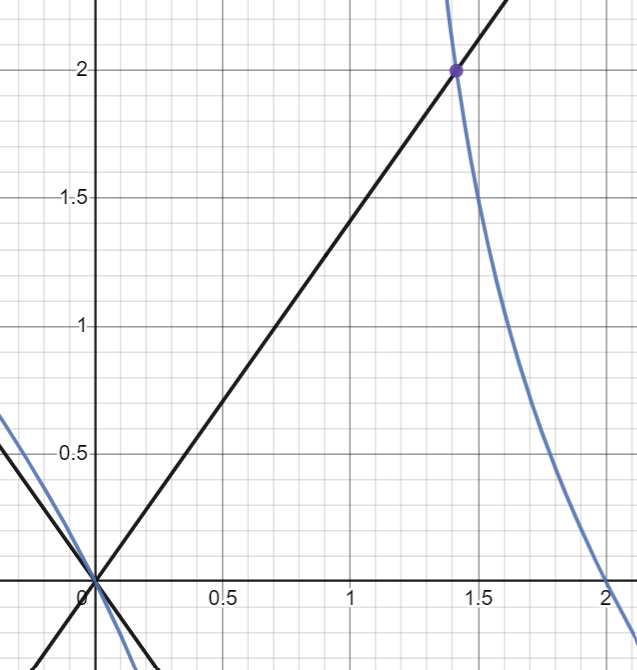
\includegraphics[scale=0.75]{Finding_Equation_Demonstration_1.png}
         \end{center}

         Based on the graph above, it looks like $f(q) = 1 +
         \frac{q}{q + 2}$ will work for our proof. And sure enough 
         it does. Furthermore, we can verify that the function we came
         up with is equivalent to that which Rudin presents.
      \end{myIndent}
   \end{itemize}

   \mySepOne{Purple}
   \hOneOld\hfill \break
   We say an ordered set $S$ has the \udefine{least upperbound
   property} if and only if when $E \subseteq S$ is nonempty and 
   bounded above, then the supremum of $E$ exists in $S$. Additionally, 
   we say an ordered set $S$ has the \udefine{greatest lower bound 
   property} if and only if when $E \subseteq S$ is nonempty and 
   bounded below, then the infimum of $E$ exists in $S$.
   
   \begin{myIndent}\begin{myIndent}\begin{myIndent}
   \begin{myIndent}\begin{myIndent}
      \teachCommentOld
      When we define the set of real numbers, this will be one of the
      fundamental properties of that set. \hfill \bigbreak
   \end{myIndent}\end{myIndent}\end{myIndent}
   \end{myIndent}\end{myIndent}

   \markLecture{1/10/2024}
   \begin{myIndent}
      \hTwoOld
      Proposition \propCount: $S$ has the least upperbound property if
      and only if $S$ has the greatest lower bound property.
      
      \hThreeOld
      \begin{myIndent}
         Proof: Let's say we have an ordered set $S$
         \hfill \bigbreak

         Assume $S$ has the least upperbound property. Then, let
         $B \subseteq S$ be a nonempty subset which is bounded below.
         Additionally, let $A \subseteq S$ be the set of all lower bounds
         of $B$. \newpage
         
         \begin{myIndent}
            We know that $A \neq \emptyset$ because we assumed that $B$ is
            bounded below. Thus, at least one lower bound to $B$ exists and
            belongs to $A$. \\Additionally, because we assumed $B$ is nonempty,
            we can say that each $b \in B$ is an upper bound to $A$. Thus, $A$
            is bounded above. Because of these two facts, we can apply the
            greatest lower bound property to say that the supremum of $A$ 
            exists. \hfill \bigbreak
   
            Let's define $\alpha \coloneq \sup{A}$. With that, our goal is 
            now to show that\\ $\alpha = \inf{B}$. To do this, we need to 
            show firstly that $\alpha$ is a lower bound to $B$ and 
            secondly that it is greater than all other lower bounds of $B$.
            \retTwo
            \begin{enumerate}
               \item For each $b \in B$, we have that $b$ is an 
                  upperbound to $A$. And since $\alpha = \sup{A}$ is the
                  least upperbound to $A$, we must have that $\alpha \leq
                  b$. Thus $\alpha$ is a lower bound to $B$. \retTwo
               
               \item If $x \in S$ is a lower bound to $B$, then $x \in A$.
                  And since\\ $\alpha = \sup{A}$, $x \leq \alpha$. This shows
                  that $\alpha$ is greater than or equal to all other lower
                  bounds. \retTwo
            \end{enumerate}
            
            Hence, $\alpha$ is the infimum of $B$. And since we did this
            for a general \\$B \subseteq S$, we can thus say that $S$ has
            the greatest lower bound property. \retTwo
         \end{myIndent}

         Now we skipped doing the reverse direction proof because it
         is almost \\ identical to the foward direction proof.
         However, just know that the above proposition is an
         \uuline{if and only if} statement. $\blacksquare$
      \end{myIndent}
   \end{myIndent}

   \mySepOne{PineGreen}
   \hOneOld\hfill \break
   A \udefine{field} is a set $F$ equipped with $2$ binary operations,
   denoted $+$ and $\cdot$, and containing two elements $0 \neq 1 \in F$
   satisfying the following conditions for all $x, y, z \in F$:

   \hTwoOld
   \begin{myIndent}
      
      \begin{tabular}{ l c }%
         {\large \textbullet} \hspace{1ex} Associativity: &
            $\begin{matrix} (x + y) + z = x + (y + z) \\ (x \cdot y) 
               \cdot z = x \cdot (y \cdot z) \end{matrix}$ \\ \\
         
         {\large \textbullet} \hspace{1ex} Commutativity: &
            $\begin{matrix} x+y=y+x\\x\cdot y = y \cdot x\end{matrix}$
               \\ \\
         
         {\large \textbullet} \hspace{1ex} Identity: &
            $\begin{matrix}0+x=x\\1\cdot x=x\end{matrix}$ \\ \\
         
         {\large \textbullet} \hspace{1ex} Inverses: &
            $\begin{matrix} \forall x\in F, \hspace{0.5em}
               \exists {-x} \in F \hspace{0.50em} s.t.
               \hspace{0.50em} x + {-x} = 0 \\ \forall x\neq 0\in F, 
               \hspace{0.5em} \exists {\displaystyle 
               \frac{1}{x}} \in F \hspace{0.50em} s.t. \hspace{0.50em} 
               x \cdot {\displaystyle \frac{1}{x}}=1\end{matrix}$ \\ \\
         
         {\large \textbullet} \hspace{1ex} Distributivity: &
            $x \cdot (y + z) = (x \cdot y) + (x \cdot z)$
      \end{tabular}
   \end{myIndent}

   \newpage
   \hOneOld
   We shall assign the following notation: 
   
   {
      \hTwoOld %  Ok so I now know that lines on the table
            % at least by default have the same color as the
            % text color.
      \centering
      \renewcommand{\arraystretch}{2.2}
      \begin{allowTableDashes}
         \begin{tabular}{ c;{10pt/3pt}c }
         
            We write \fillInBlank{1} \hspace{0.75em} & 
               \hspace{0.75em} to mean \fillInBlank{1} \\ \hline
            
            $x-y$ & $x + {-y}$ \\ \hdashline[10pt/3pt]

            ${\displaystyle \frac{x}{y}}$ & $x \cdot 
                  {\displaystyle \frac{1}{y}}$\\[8pt] \hdashline[10pt/3pt]
            
            $2$ & $1 + 1$\\ \hdashline[10pt/3pt]

            $2x$ & $x + x$\\ \hdashline[10pt/3pt]

            $x^2$ & $x \cdot x$\\ \hdashline[10pt/3pt]

            $xy$ & $x\cdot y$
         \end{tabular}
      \end{allowTableDashes}
      \par
   }
   \retTwo
   
   \hOneOld
   Now what follows is a number of propositions concerning the 
   arithmetic properties of a field...
   
   \begin{myIndent}
      \hTwoOld
      \resetSubPropCount
      For a field $F$ and elements $x,y,z\in F$, we have the
      following propositions:
      
      Proposition \propCount.\subPropCount: $x+y=x+z \Rightarrow y=z$
      {\hThreeOld
      \begin{myIndent}
         Proof: Assume $x+y=x+z$. Then...
            \begin{myIndent}
               \renewcommand{\arraystretch}{1.4}
               \begin{tabular}{ l c }
                  $y=0+y$ & (addition identity property)\\
                  $\hphantom{y}=({-x}+x)+y$ & (addition inverse property)\\
                  $\hphantom{y}={-x}+(x+y)$ & (addition associative property)\\
                  $\hphantom{y}={-x}+(x+z)$ & (by our assumption)\\
                  $\hphantom{y}=({-x}+x)+z$ & (addition associative property)\\
                  $\hphantom{y}=0+z$ & (addition inverse property)\\
                  $\hphantom{y}=z$ & (addition identity property)
               \end{tabular}
            \end{myIndent}
      \end{myIndent} \retTwo}

      Proposition \propCount[0].\subPropCount: $x+y=x \Rightarrow y=0$
      {\hThreeOld
      \begin{myIndent}
         Proof: Plug in $z=0$ into proposition 2.1. in order to get
         that $y=z=0$.
      \end{myIndent} \retTwo}

      Proposition \propCount[0].\subPropCount: $x+y=0 \Rightarrow y={-x}$
      {\hThreeOld
      \begin{myIndent}
         Proof: Plug in $z={-x}$ into proposition 2.1. in order to get
         that\\ $y=z={-x}$.
      \end{myIndent} \retTwo}

      Proposition \propCount[0].\subPropCount: ${-(-x)}=x$
      {\hThreeOld
      \begin{myIndent}
         Proof: Observe that $x+{-x}={-x}+x=0$ by the inverse and\\ 
         commutative properties of addition. Then, by proposition
         2.3, we know that ${-x}+x=0 \Rightarrow x={-(-x)}$.
      \end{myIndent}}
      \newpage
      Proposition \propCount[0].\subPropCount: $x\cdot y=x\cdot z 
                                    \text{ and } x\neq0\Rightarrow y=z$
      {\hThreeOld
      \begin{myIndent}
         Proof: Assume $x\cdot y=x\cdot z$ and $x\neq0$. Then...
            \begin{myIndent}
               \renewcommand{\arraystretch}{1.4}
               \begin{tabular}{ l c }
                  $y=1\cdot y$ & (multiplication identity property)\\
                  $\hphantom{y}=(\frac{1}{x}\cdot x)\cdot y$ & 
                                 (multiplication inverse property)\\
                  $\hphantom{y}=\frac{1}{x}\cdot(x\cdot y)$ & 
                                 (multiplication associative property)\\
                  $\hphantom{y}=\frac{1}{x}\cdot(x\cdot z)$ & 
                                 (by our assumption)\\
                  $\hphantom{y}=(\frac{1}{x}\cdot x)\cdot z$ & 
                                 (multiplication associative property)\\
                  $\hphantom{y}=1\cdot z$ & 
                                 (multiplication inverse property)\\
                  $\hphantom{y}=z$ & 
                                 (multiplication identity property)
               \end{tabular}
               \retTwo
            
         \begin{myIndent}\begin{myIndent}\begin{myIndent}
            \teachCommentOld
            Note that to use the multiplication inverse\\ property,
            we have to assume $x \neq 0$ !!
         \end{myIndent}\end{myIndent}\end{myIndent}

         \end{myIndent}
      \end{myIndent} \retTwo}

      Proposition \propCount[0].\subPropCount: $x\cdot y=x \Rightarrow y=1$
      {\hThreeOld
      \begin{myIndent}
         Proof: Plug in $z=1$ into proposition 2.5. in order to get
         that $y=z=1$.
      \end{myIndent} \retTwo}

      Proposition \propCount[0].\subPropCount: $x\cdot y=1 \Rightarrow 
               y={\displaystyle\frac{1}{x}}$
      {\hThreeOld
      \begin{myIndent}
         Proof: Plug in $z={\frac{1}{x}}$ into proposition 2.5. in order to get
         that\\ $y=z={\frac{1}{x}}$.
      \end{myIndent} \retTwo}

      Proposition \propCount[0].\subPropCount:
         ${\dfrac{\hspace{0.15em}1\hspace{0.15em}}{
            \frac{1}{x}}} = x$
      {\hThreeOld
      \begin{myIndent}
         Proof: Observe that $x\cdot{\frac{1}{x}}=
         {\frac{1}{x}}\cdot x=1$ 
         by the inverse and commutative \\[3pt] properties of multiplication. 
         Then, by proposition 2.7, we know that \\[3pt]
         ${\frac{1}{x}}\cdot x=1 \Rightarrow x={
         \dfrac{\hspace{0.15em}1\hspace{0.15em}}{\frac{1}{x}}}$.
      \end{myIndent} \retTwo}

      Proposition \propCount[0].\subPropCount: $0\cdot x = 0$
      {\hThreeOld
      \begin{myIndent}
         Proof: $(0\cdot x) + (0\cdot x) = (0+0)\cdot x = 0\cdot x$.
         Thus we have an expression of the form $a+b=a$ which we can use
         proposition 2.2 on. Hence, we can conclude $0\cdot x=0$.
      \end{myIndent} \retTwo}

      Proposition \propCount[0].\subPropCount: 
         $x\neq0 \text{ and } y\neq0 \Rightarrow x\cdot y \neq 0$
      {\hThreeOld
      \begin{myIndent}
         Proof: since $x, y\neq0$, we can say that $x\cdot y \cdot
         {\frac{1}{x}} \cdot {\frac{1}{y}}
         = 1 \neq 0$. Now by proposition 2.9, $x\cdot y=0 \Rightarrow
         (x\cdot y)\cdot\left({\frac{1}{x}} \cdot 
         {\frac{1}{y}}\right)=0$. However, we know that is not the
         case. So $x\cdot y$ can't equal zero.
      \end{myIndent} \retTwo}
   \end{myIndent}
   \newpage
   
   \markLecture{1/12/2024}
   
   {\begin{myIndent} \hTwo
   Proposition \propCount[0].\subPropCount: $({-x})y={-(xy)}=x({-y})$
      {\hThree
      \begin{myIndent}
         Proof: $xy+({-x})y=(x+{-x})y=0y=0$. Thus by proposition 2.3,\\
         $({-x})y={-(xy)}$. We can make a similar argument to also say
         that\\ $x({-y})={-(xy)}$.
      \end{myIndent} \retTwo}

      Proposition \propCount[0].\subPropCount: $({-x})({-y})=xy$
      {\hThree
      \begin{myIndent}
         Proof: Using proposition 2.11, we can say that \\
         $({-x})({-y}) = {-(x({-y}))} = {-({-(xy)})}$. Then
         by proposition 2.4, we can \\conclude ${-({-(xy)})} = xy$.
      \end{myIndent} \retTwo}
   \end{myIndent}}
   
   \mySepOne{Black}


   An \udefine{ordered field} is a field $F$ equipped with an ordering
   $<$ satisfying $\forall x,y,z \in F$:
   
   \begin{myIndent}\begin{myIndent}
      \begin{enumerate}
         \item[OF1.] $y<z \Rightarrow y+x<z+x$
         \item[OF2.] $(x>0 \text{ and } y>0) \Rightarrow xy>0$ 
      \end{enumerate}
   \end{myIndent}\end{myIndent} \retTwo

   For $x$ in an ordered field, we call $x$ \udefine{positive} if and 
   only if $x>0$. Similarly, we call $x$ \udefine{negative} if and
   only if $x<0$.

   {\begin{myIndent} \hTwo
   Proposition \propCount: For an ordered field $F$ and 
      $x, y, z \in F$, we have:

      \begin{enumerate}
         \item $x<y \Leftrightarrow {-y}<{-x}$
         {\begin{myIndent} \hThree
            Proof: By property OF1 of an ordered field, we can
            say that\\ $x<y\Rightarrow x+({-x}+{-y})<y+({-x}+{-y})
            \Rightarrow -y < -x$. \retTwo
         \end{myIndent}}

         \item $(x>0 \text{ and } y<z) \Rightarrow xy<xz$
         {\begin{myIndent} \hThree
            Proof: By property OF1 of an ordered field, $y<z
            \Rightarrow y-y<z-y$. Or in other words, $0<z-y$.  
            Therefore, since $x$ is also positive by assumption,
            property OF2 of an ordered field tells us that
            $x(z-y)>0$. Finally, adding $xy$ to both sides by property
            OF1 and then distributing gives us: \\$xz-xy+xy=xz<xy$.
            \retTwo
         \end{myIndent}}

         \item $(x<0 \text{ and } y<z) \Rightarrow xy>xz$
         {\begin{myIndent} \hThree
            Proof: Since $x<0$, we have $-x>0$ by proposition 3.1.
            Then by applying proposition 3.2, we know that
            $(-x>0 \text{ and } y<z) \Rightarrow -xy<-xz$.
            Finally, by reapplying proposition 3.1, this becomes
            $xy>xz$.\retTwo
         \end{myIndent}}

         \item $x \neq 0 \Rightarrow x^2 > 0$
         {\begin{myIndent} \hThree
            Proof: If $x>0$, then $x^2=xx>0x=0$ by property OF2
            of an \\ordered field. Meanwhile, if $x<0$, then $-x>0$
            by proposition 3.1. So $(-x)(-x)>0$ by property OF2.
            But $(-x)(-x)=x^2$ by proposition 2.12. So $x^2>0$.
            \retTwo
         \end{myIndent}}
         \newpage

         \item $0<x<y \Rightarrow 0<\frac{1}{y}<\frac{1}{x}$
         {\begin{myIndent} \hThree
            Proof: Since $y>0$ and $y\cdot\frac{1}{y}=1>0=0\cdot\frac{1}{y}$,
            we must have $\frac{1}{y}>0$ by propositions 3.2 and 3.3.
            Note that $\frac{1}{y}\neq0$ because if it did,
            $y\cdot\frac{1}{y}=0$. \\ Similarly, we can show $\frac{1}{x}
            >0$. Now multiply both sides of $x<y$ by the positive element
            $\frac{1}{x}\cdot\frac{1}{y}$ and apply proposition 3.2
            to get that $\frac{1}{y}<\frac{1}{x}$.
            \retTwo
         \end{myIndent}}
      \end{enumerate}
   \end{myIndent}}

   \mySepTwo[Black]

   \hOne
   \uuline{Theorem}: There is (up to isomorphism) precisely one ordered field that contains $\mathbb{Q}$ and has the least upper bound property.
   We denote this field $\mathbb{R}$ and we call its elements 
   \udefine{real numbers}.
   
   \begin{myIndent}\begin{myIndent}\begin{myIndent}\begin{myIndent}
   \begin{myIndent}\begin{myIndent}
      {\teachComment
         In other words, this theorem is stating that $\mathbb{R}$ exists and is unique. Unfortunately, the proof for this is very long and so won't be covered in lecture. However, the professor has left some resources to cover it. So, I will have the proof of this theorem later in these notes. \newline
            See page: {\color{BrickRed} <research how to cite a page>}
      }
   \end{myIndent}\end{myIndent}
   \end{myIndent}\end{myIndent}\end{myIndent}\end{myIndent}

   \mySepTwo[Black]

   
   {\begin{myIndent} \hTwo \resetSubPropCount
      Proposition \propCount.\subPropCount: If $x\in\mathbb{R}$, $y\in\mathbb{R}$, and $x>0$, then there is a positive integer $n$ such that $nx>y$. This is called the \udefine{archimedean property}.

      {\begin{myIndent} \hThree
         Proof: We proceed by looking for a contradiction. Let $A=\{nx \mid n\in\mathbb{Z}^+\}$ and assume $\nexists n\in\mathbb{Z}^+$ such that $nx>y$. In that case we know $y$ is an \\upper bound of $A$. Additionally, since $A$ is bounded above, we know by the least upper bound property of the real numbers that $\sup{A}$ exists. So, let $\alpha=\sup{A}$. \retTwo

         Now because $\mathbb{R}$ is an ordered field, we know that: \\
         $x>0 \Rightarrow -x<0 \Rightarrow \alpha-x<\alpha$. Therefore, because $\alpha$ is the least upper bound, we know that $\alpha - x$ is not an upper bound for $A$. Or in other words, there exists $n\in\mathbb{Z}^+$ such that $nx>\alpha-x$. But this contradicts that $\alpha$ is the least upper bound of $A$ because $nx>\alpha-x \Rightarrow (n+1)x>\alpha$ and $(n+1)x\in A$. So we conclude that the supremum of $A$ can't exist, which by the contrapositive of the least upper bound property, means that $A$ is not bounded above.
         \retTwo
      \end{myIndent}}

      Proposition \propCount[0].\subPropCount: If $x, y\in\mathbb{R}$ and $x<y$, then there exists a $p\in\mathbb{Q}$ such that\\ $x<p<y$. In other words, we say that $\mathbb{Q}$ is \udefine{dense} in $\mathbb{R}$.

      {\begin{myIndent} \hThree
         Proof: Since $x<y$, we have that $0<y-x$. Then because $y-x$ is positive, we can use the archimedean property to say that there exists an integer $n$ such that $n(y-x)>1$. Note for later that this means $ny>1+nx$.

         \newpage

         Now note that since $1>0$ and $nx$ is a real number, we can use the archimedean property twice to get positive integers $m_1$ and $m_2$ such that $m_1\cdot1>-nx$ and $m_2\cdot1>+nx$. Thus, we get the expression $-m_1 < nx < m_2$. So now \\consider the set $B = \{m \in \mathbb{Z} \mid -m_1 \geq nx \geq m_2 \text{ and } m>nx\}$. We know that $B$ has finitely many elements and that $B$ contains at least one \\element: $m_2$. So $B$ must have a minimum element. We'll refer to that \\minimum element as $m$. Notably, as $m$ is the minimum element of $B$, we know that $m-1 \notin B$, meaning that $m-1\leq nx < m$ \retTwo

         We now combine inequalities as follows: $m-1 \leq nx \Rightarrow m \leq nx+1$. So we have that $nx < m \leq nx+1$. But now remember from the previous page that $ny>1+nx$. So we can say that $nx < m \leq nx+1 < ny$. Finally, because $n>0$, we can multiply the inequality by $\frac{1}{n}$ to get that $x<\frac{m}{n}<y$. $\blacksquare$

      \end{myIndent}}
   \end{myIndent}}
   \mySepTwo \newline
   \markLecture{1/17/2024} \newline
   \uuline{Theorem}: If $x\in\mathbb{R}$, $x>0$, $n\in\mathbb{Z}$, and $n>0$, then there is a unique $y\in \mathbb{R}$ with $y>0$ and $y^n=x$. This number $y$ is denoted $\sqrt[n]{x}$ or $x^\frac{1}{n}$. \retTwo

   {\begin{myIndent} \hTwo
      To prove this, first note the following lemma about positive integers $n$ and $a, b\in\mathbb{R}$:
      
      {\centering $b^n-a^n=(b-a)(b^{n-1}+ab^{n-2}+\ldots+a^{n-2}b+a^{n-1})$ \par}

      To prove this, one can either use induction or just calculate it out by hand to verify that the equality holds. \retTwo

      Additionally, also consider that if $n$ is a positive integer and $0\leq a \leq b$ where \\ $a,b\in\mathbb{R}$, then we have that $a^n\leq b^n$. Combining this fact with the lemma above, we can say that $0\leq a \leq b$ implies that $b^n-a^n \leq (b-a)nb^{n-1}$. Or in other words: $a^n \leq b^n \leq a^n + (b-a)nb^{n-1}$.
      {\teachComment  \begin{myTindent}\begin{myDindent}
         This comes from replasing every $a$ in the expression \\$(b^{n-1}+ab^{n-2}+\ldots+a^{n-2}b+a^{n-1})$ with $b$ in order to get that $b^n-a^n \leq (b-a)(b^{n-1} + b^{n-1} + \ldots + b^{n-1})$
      \end{myDindent}\end{myTindent}} \retTwo

      Now set $E=\{t\in\mathbb{R} \mid t>0, t^n\leq x\}$.
      {\begin{myIndent} \hThree
         We can show that $E$ is nonempty...
         \begin{itemize}
            \item If $x \geq 1$, then $t=1 \in E$ since $1^n=1\leq x$.
            \item If $x < 1$, then $x\in E$ since $x<1 \Rightarrow x^{n-1}<1^{n-1}=1$. But then $x^n<x$.
         \end{itemize}
         Thus, we know $E \neq \emptyset$. \retTwo

         We can also show that $E$ is bounded above. Consider $t=1+x$. In that case, $t>1$, which implies that $t^{n-1} > 1^{n-1} = 1$. Therefore, $t^n > t$, meaning that $t^n > x$. So $t=x+1$ is an upper bound for $E$.
         \newpage
         Thus by the least upper bound property of the real numbers, we know \\$y = \sup{E}$ exists. \retTwo
      \end{myIndent}}

      \uuline{Claim 1}: $y^n \geq x$.
      
      {\begin{myIndent} \hThree
         To prove this, we shall procede towards a contradiction. Assume $y^n<x$\retTwo
         
         Then pick some $h$ such that $0<h<\gamma$ and $\gamma$ is some mystery constant for us to find. Then, we can say that $y<y+h$, meaning by the lemma on the previous page that $y^n \leq (y+h)^n \leq y^n + (y+h-y)n(y+h)^n-1$. Or in other words, $(y+h)^n \leq y^n + hn(y+h)^n-1$. \retTwo

         Now we shall make our first assumption about $\gamma$: let $\gamma \leq 1$. That way, we know that $(y+h)^n \leq y^n + hn(y+h)^n-1 < y^n + hn(y+1)^n$. And since, we are assuming that $y^n<x$, we know there must exist some value of $h$ such that $y^n + hn(y+1)^{n-1} < x$. Putting this limitation on $h$, we get that $h < \frac{x - y^n}{n(y+1)^{n-1}}$ (Remember that $x-y^n$, $y$, and $n$ are all positive). So finally, we say that $\gamma = \min{\left( 1, \frac{x - y^n}{n(y+1)^{n-1}} \right)}$. This is so that for $0<h<\gamma$, we have that $(y+h)^n < x$. \retTwo

         Thus, we have a contradiction as we assumed that $y$ is the supremum of $E$ and yet we just proved that $y+h \in E$. So, $y^n$ cannot be less than $x$, meaning that that $y^n \geq x$. \retTwo
      \end{myIndent}}

      \uuline{Claim 2}: $y^n \leq x$.
      
      {\begin{myIndent} \hThree
         To prove this, we shall again proceed towards a contradiction. Assume \\$y^n>x$. \retTwo

         Then for some $h$ such that $0<h<\gamma$ where $\gamma$ is a new mystery constant, consider $y-h$. \retTwo

         
         {\begin{center} \hFour
            \begin{myClosureOneDeprecated}{5}
               I now realize that I need to prove this lemma: for a positive integer $n$ and real numbers $a$ and $b$ such that $a \geq b$, we have that \\$(a-b)^n \geq a^n-bna^{n-1}$. We can prove this through induction. \\ \\
               Firstly for $n=1$: we have that $(a-b)^1 = a^1 - b(1)a^0$. \\ \\
               Now assume that for $k\geq 1$, $(a-b)^k \geq a^k - bka^{k-1}$.\\ Then $(a-b)^{k+1} = (a-b)(a-b)^k$. And since $(a-b)>1$, we know that $(a-b)^{k+1} = (a-b)(a-b)^k \geq (a-b)(a^k - bka^{k-1})$. \\ \\

               Now let's expand out our lesser term to get that: \\ $(a-b)^{k+1} \geq a^{k+1}-bka^k - ba^k + b^2ka^{k-1}$. Thus, we know that \\$(a-b)^{k+1} \geq a^{k+1}-b(k+1)a^k + b^2ka^{k-1} > a^{k+1}-b(k+1)a^k$. Hence, we have shown that $(a-b)^{k+1} \geq a^{k+1}-b(k+1)a^k$.
            \end{myClosureOneDeprecated}
         \end{center}}
         \newpage

         Based on the lemma covered right before this, we have that \\$(y-h)^n \geq y^n-hny^{n-1}$. But now let's require that $y^n-hny^{n-1}>x$. Thus, we can say that $h<\frac{y^n-x}{ny^{n-1}}$. \retTwo

         So setting $\gamma = \frac{y^n-x}{ny^{n-1}}$, we have that for $0 < h < \gamma$, \hspace{0.25em} $(y-h)^n > x$. But this now leads to a contradiction as $y-h$ must be an upper bound to $E$.
         {\begin{myIndent} \hFour
            (If some number $z$ is greater than $y{-h}$, than $z^n > (y{-h})^n > x$. So $z \notin E$.) \newline
         \end{myIndent}}
         However, $y-h$ can't be an upper bound to $E$ as we specified that $y$ is the least upper bound of $E$. So we conclude that $y^n$ cannot be greater than $x$, thus meaning $y^n \leq x$.
      \end{myIndent}}

      So since $y^n \leq x$ and $y^n \geq x$, we conclude that $y^n = x$.
      \retTwo

      Finally, we now shall mention that $y$ is obviously the unique number such that \\$y^n=x$. After all, for $0<a<y<b$, we have that $a^n < y^n < b^n$. So, there can only be one number $y$ such that $y^n=x$.
   \end{myIndent}}

   \mySepTwo \newline
   \markLecture{1/19/2024}

   \uuline{Decimal representations of real numbers}:
   \begin{itemize}
      \item Each $x \in \mathbb{R}$ such that $x>0$ can be written $x=n_0.n_1n_2n_3\ldots$ where $n_0 \in \mathbb{Z}$ and $\forall i \geq 1$, $n_i \in \{0,1,2,3,4,5,6,7,8,9\}$.
      {\begin{myIndent} \hTwo
         Specifically, let $n_0$ be the largest integer with $n\leq x$. Then inductively, pick $n_k$ to be the max element in $\{0,1,2,3,4,5,6,7,8,9\}$ such that: \[
            n_0 + \frac{n_1}{10} + \cdots + \frac{n_{k-1}}{10^{k-1}} + \frac{n_k}{10^k} \leq x\]
      \end{myIndent}}
      
      \item Conversely, suppose $n_0 \in \mathbb{Z}$ and $\forall i \geq1, n_i \in \{0,1,2,3,4,5,6,7,8,9\}$. Then, defining $E=\{n_0, n_0 + \frac{n_1}{10}, \ldots, n_0 + \frac{n_1}{10} + \cdots + \frac{n_k}{10^k}, \ldots\}$, we have that\\ $n_0.n_1n_2n_3\ldots = x\in\mathbb{R}$ where $x = \sup{E}$.
   \end{itemize} \retTwo

   We will rarely ever use decimal representations though.

   \newpage

   The \uuline{extended real number system} is the set $\mathbb{R} \cup \{{-\infty}, {+\infty}\}$ where for all $x\in\mathbb{R}$:
   {\hTwo \begin{tabular}{ p{1.7in} p{2.2in} p{2.2in} }
      \begin{itemize}
         \item $-\infty < x < +\infty$
         \item $x + \infty = +\infty$
         \item $x - \infty = {-\infty}$
         \item $\frac{x}{+\infty} = 0 = \frac{x}{-\infty}$
      \end{itemize}
      &
      \begin{itemize}
         \item $x>0 \Rightarrow x(+\infty)=+\infty$
         \item $x>0 \Rightarrow x(-\infty)=-\infty$
         \item $+\infty +\infty = +\infty$
         \item $+\infty(+\infty) = +\infty$ 
      \end{itemize}
      &
      \begin{itemize}
         \item $x<0 \Rightarrow x(+\infty)=-\infty$
         \item $x<0 \Rightarrow x(-\infty)=+\infty$
         \item $-\infty - \infty = -\infty$
         \item $+\infty(-\infty) = -\infty$ 
      \end{itemize}
   \end{tabular}}
   {\begin{myTindent} \hFour
      All other operation involving $+\infty$ and $-\infty$ are left undefined. \retTwo
   \end{myTindent}}

   \diamond \hspace{0.5em} Sometimes, we denote the extended real number system $\overbar{\mathbb{R}}$.

   \diamond \hspace{0.5em} The extended real number system is not a field.

   \diamond \hspace{0.5em} To distinguish $x\in\mathbb{R}$ from $\infty$ or $-\infty$, we call $x\in\mathbb{R}$ finite.

   \mySepTwo

   The set of \udefine{complex numbers}, denoted $\mathbb{C}$, is the set of all things of the form $a+bi$ where $a, b \in \mathbb{R}$ and $i$ is a symbol satisfying $i^2=-1$.
   
   {\teachComment \begin{myTindent}\begin{myIndent}
      To be more rigorous about this definition, what we would do is define the set of complex numbers to be the set of pairs of real numbers equipped with the following operations:
      \begin{myIndent}
         For $z, u \in \mathbb{C}$ such that $z=(a, b)$ and $u=(c, d)$:
         \begin{itemize}
            \item $z+u = (a+c, b+d)$
            \item $z\cdot u = (ac - bd, ad+bc)$ \newline
         \end{itemize}
      \end{myIndent}
      Having done that, we would then:
      \begin{enumerate}
         \item Define $0 = (0, 0)$ and $1 = (1, 0)$
         \item Prove that $\mathbb{C}$ satisfies our field axioms
         \item Say that $i = (0, 1)$ and then show that $i^2 = (-1, 0)$
         \item And finally show that for $a, b \in \mathbb{R}$, \hspace{0.25em} $a(1) + b(i) = (a, b)$ 
         
         \begin{myTindent}\begin{myTindent}
            (Thus it makes sense to denote $z \in \mathbb{C}$ as $z = a + bi$)
         \end{myTindent}\end{myTindent} \retTwo
      \end{enumerate}

      However, we're behind and so not going to spend time doing that in class. \retTwo
   \end{myIndent}\end{myTindent}}
   
   For $z= a+bi$, we denote $\rea{z} = a$ the \udefine{real} part of $z$. On the other hand, we denote $\ima{z} = b$ the \udefine{imaginary} part of $z$. \retTwo

   The \udefine{complex conjugate} of $z=a+bi$ is $\overbar{z}=a-bi$.
   \newpage
   
   \begin{tabular}{ p{3.2in} p{2.8in} }
      {\hTwo \begin{myIndent}
         Proposition \propCount: If $z, w \in \mathbb{C}$, then:
         \begin{enumerate}
            \item $\overbar{z+w}=\overbar{z}+\overbar{w}$
            \item $\overbar{zw} = \overbar{z}\cdot \overbar{w}$
            \item $z + \overbar{z} = 2\rea{z}$
            \item $z - \overbar{z} = 2\ima{z}i$
            \item $z\overbar{z} \in \mathbb{R}$ and $z\overbar{z} > 0$ when $z\neq 0$. 
         \end{enumerate}
      \end{myIndent}}
      &
      \hThree
      \begin{myClosureOneDeprecated}{2.8}
         {Proof: \newline
            \hFour
            Points 1-4 can be verified by direct\newline computation.\newline  As for point 5, note that if $z = a+bi$, then\newline $z\overbar{z} = (a+bi)(a-bi) = a^2+b^2$.\newline Now as $a, b\in\mathbb{R}$, we know that \newline $a^2+b^2\in\mathbb{R}$. But $a^2+b^2 > 0$ if $b\neq a\neq0$. Meanwhile, $a^2+b^2=0$ if $a=b=0$. So $z\overbar{z} > 0$ if $z\neq0$
         }
      \end{myClosureOneDeprecated}
   \end{tabular} \retTwo
   
   The \udefine{absolute value} of $z=a+bi$ is $\lvert z\rvert = \sqrt{z\myBar{z}}$

   \begin{myIndent} \hTwo
      Propostion \propCount: For $z, w \in \mathbb{C}$, we have that:

      \begin{enumerate}
         \item $\lvert 0 \rvert = 0$ and $\lvert z \rvert > 0$ when $z\neq0$.
         \item $\lvert z \rvert = \lvert \overbar{z} \rvert$
         \item $\lvert zw \rvert = \lvert z \rvert\lvert w \rvert$
         \item $\lvert \rea{z} \rvert \leq \lvert z \rvert$
         \item $\lvert \ima{z} \rvert \leq \lvert z \rvert$
         \item $\lvert z + w \rvert \leq \lvert z \rvert + \lvert w \rvert$
         {\begin{myDindent} \teachComment
            This last bullet is the \uuline{triangle inequality}.
         \end{myDindent}}
      \end{enumerate}

      {\begin{myIndent} \hThree
         Proof:\\
         Claims 1, 2, and 3 can be verified through direct computation. \retTwo

         To prove claim 4, note that $a^2 \leq a^2+b^2$. So, $\lvert a \rvert = \sqrt{a^2} \leq \sqrt{a^2+b^2} = \lvert z \rvert$. We can repeat this but with $b^2$ to prove claim 5. \retTwo

         Lastly, to prove claim 6, note that $\lvert z+w\rvert^2=(z+w)(\overbar{z+w})=(z+w)(\overbar{z}+\overbar{w})$. Now, we can distribute to get that $\lvert z+w\rvert^2= z\overbar{z} + z\overbar{w} + w\overbar{z} + w\overbar{w}$. So, we know that $\lvert z+w\rvert^2 = \lvert z \rvert^2 + z\overbar{w} + w\overbar{z} + \lvert w \rvert^2$. \retTwo

         But now observe that $w\overbar{z} = \overbar{z\myBar{w}}$. So $z\overbar{w} + w\overbar{z} = 2\rea{z\overbar{w}}$. But by claim 4, we know that $\rea{z\overbar{w}}\leq \lvert z\overbar{w} \rvert$. Additionally, by claims 2 and 3, we have that\\ $\lvert z\overbar{w} \rvert = \lvert z \rvert\lvert \overbar{w} \rvert = \lvert z \rvert\lvert w \rvert$. So, we know that $\lvert z+w\rvert^2 \leq \lvert z \rvert^2 + 2\lvert z \rvert\lvert w \rvert + \lvert w \rvert^2$. This simplifies to $\lvert z+w\rvert^2 \leq (\lvert z \rvert + \lvert w \rvert)^2$. Hence, $\lvert z + w \rvert \leq \lvert z \rvert + \lvert w \rvert$.
      \end{myIndent}}
   \end{myIndent}

   \newpage
   \markLecture{1/22/2024}

   {\begin{myIndent} \hTwo
      \uuline{Theorem}: (the Cauchy-Schwarz Inequality)
      \begin{myIndent}
         If $a_1, \ldots, a_n, b_1, \ldots, b_n \in \mathbb{C}$, then: \[
            \left|\sum_{j=1}^n a_j\overbar*{b_j} \right|^2 \leq \sum_{j=1}^n\lvert a_j \rvert^2\sum_{j=1}^n\lvert b_j \rvert^2\]
            \retTwo
            \retTwo
            \hThree
            Proof:\\
            Define ${\displaystyle A = \sum_{j=1}^n\lvert a_j\rvert^2_,} \quad {\displaystyle B =\sum_{j=1}^n\lvert b_j\rvert^2_,} \hspace{0.5em}\text{and}\hspace{0.5em} {\displaystyle C =\sum_{j=1}^n{a_j\overbar*{b_j}}_.}$\\

            Note that $A, B \in \mathbb{R}$ such that $A, B \geq 0$. Meanwhile, $C \in \mathbb{C}$. \retTwo

            If $B = 0$, then $b_1 = \ldots = b_n = 0$. Thus $C = 0$ as well and so the inequality is trivially true. \retTwo
            So now consider if $B > 0$. Then we can make a series of manipulations \\starting with: $0 \leq {\displaystyle \sum_{j=1}^n\lvert Ba_j - Cb_j\rvert^2_.}$ 
            {\teachComment 
            \begin{myTindent}\begin{myTindent}
               (The professor said not to worry about how Rudin thought of using this formula.) \retTwo
            \end{myTindent}\end{myTindent}}

            \begin{center}
               \begin{tabular}{ r c l }
                  $0$ & $\leq$ & ${\displaystyle \sum_{j=1}^n\lvert Ba_j - Cb_j\rvert^2 }$ \\ \\
                  & $=$ & ${\displaystyle \sum_{j=1}^n{(Ba_j - Cb_j)(B\overbar*{a_j} - \overbar*{C}\overbar*{b_j})} }$ \\ \\
                  & $=$ & ${\displaystyle B^2 \sum_{j=1}^n\lvert a_j \rvert^2 - BC\sum_{j=1}^n{\overbar*{a_j}b_j} - B\overbar{C}\sum_{j=1}^n{a_j\overbar*{b_j}} + \lvert C \rvert^2\sum_{j=1}^n\lvert b_j \rvert^2}$ \\
                  & $ = $ & ${\displaystyle B^2A - BC\overbar{C} - B\overbar{C}C + \lvert C \rvert^2B}$ \\
                  & $ = $ & ${\displaystyle B^2A - B \lvert C \rvert^2}$ \\
                  & $ = $ & ${\displaystyle B(AB - \lvert C \rvert^2)}$
               \end{tabular}
            \end{center}
            \retTwo
            Thus, since we're assuming $B > 0$, we know that $AB - \lvert C \rvert^2 \geq 0$.\\ So, $AB \geq \lvert C \rvert^2$. $\blacksquare$
      \end{myIndent}
   \end{myIndent}}

   \newpage

   We call elements $\mVec{x} = (x_1, x_2, \ldots, x_k) \in \mathbb{R}^k \hspace{0.5em}$ \udefine{vectors} or \udefine{points}. The $x_i$ are the\\ \udefine{coordinates} of $\mVec{x}$. \retTwo

   The \udefine{inner product} or \udefine{dot product} of $\mVec{x}$, $\mVec{y} \in \mathbb{R}^k \hspace{0.4em}$ is: $\hspace{0.4em} {\displaystyle \mVec{x} \cdot \mVec{y} = \sum_{i=1}^k{x_iy_i}}$\retTwo

   The \udefine{norm} of $x \in \mathbb{R}^k$ is $\| \mVec{x} \| = (\mVec{x} \cdot \mVec{x})^\frac{1}{2}$

   {\begin{myIndent} \hTwo
      \begin{tabular}{ p{3.5in} p{2.5in}}
         Proposition \propCount: If $\mVec{x}, \mVec{y}, \mVec{z} \in \mathbb{R}^k$ and $\alpha \in \mathbb{R}$, then:
         \begin{enumerate}
            \item $\| \mVec{0} \| = 0$ and $\| \mVec{x} \| > 0$ when $\mVec{x} \neq \mVec{0}$.
            \item $\| \alpha \mVec{x} \| = \alpha \| \mVec{x} \| $
            \item $\| \mVec{x} \cdot \mVec{y} \| \leq \| \mVec{x} \| \| \mVec{y} \|$
            \item $\| \mVec{x} + \mVec{y} \| \leq \| \mVec{x} \| + \| \mVec{y} \|$
            \item  $\| \mVec{x} - \mVec{z} \| \leq \| \mVec{x} - \mVec{y} \| + \| \mVec{y} - \mVec{z} \|$
         \end{enumerate}
         & \hFour \retTwo
         The proofs for 1-4. are nearly \newline identical to those for complex \newline numbers so we won't cover them\newline here.\retTwo As for 5, note that\newline $\mVec{x} + (-\mVec{z}) = \mVec{x} - \mVec{y} + \mVec{y} - \mVec{z}$.
      \end{tabular}
   \end{myIndent}}
   \retTwo
   \mySepOne{Black}

   For sets $X$, $Y$ and a function $f: X\rightarrow Y$, we shall write:
   \begin{itemize}
      \item for $A \subseteq X, \hspace{0.5em} f(A) = \{f(a) \mid a\in A\}\quad$
         {\color{BrickRed} (This is the image of $A$.)}
      
      \item for $B \subseteq Y, \hspace{0.5em} f^{-1}(B)=\{x\in X \mid f(x)\in B\} \quad$
         {\color{BrickRed} (This is the preimage of $A$.)}

      \item for $y \in Y$, we write $f^{-1}(y)$ for $f^{-1}(\{y\})$
   \end{itemize}
   \retTwo
   We say two sets $A$ and $B$ have \udefine{equal cardinality}, denoted $\lvert A \rvert = \lvert B \rvert$ if there is a bijection $f$ from $A$ onto $B$. 
   
   \begin{myIndent}
      \begin{itemize}
         \item $A$ is \udefine{finite} if it has equal cardinality with $\{1, \ldots, n\}$ for some $n \in \mathbb{Z}^+$ or if $A = \emptyset$.
         \item $A$ is \udefine{countable} if either $A$ is finite or $A$ has equal cardinality with $\mathbb{Z}^+$.
         \item $A$ is \udefine{uncountable} if its not countable.
      \end{itemize} \retTwo
   \end{myIndent}

   A \udefine{sequence} is a function $f$ having domain $\mathbb{Z}^+$. If $f(n) = x_n \in A$ for each integer $n$,\\ it is typical to denote $f$ by $(x_n)_{n \in \mathbb{Z}^+}$ or more simply by $(x_n)$. \retTwo
   {\hTwo
   \begin{myIndent}
      Proposition \propCount: If $A$ is countable and $E \subseteq A$, then $E$ is countable.
      {\hThree
      \begin{myIndent}
         Proof:\\
         If $E$ is finite, then $E$ is countable and we're done. So assume $E$ is infinite. Then as $E \subseteq A$, we know $A$ is infinite as well.
         \newpage
         Since $A$ is countable, we can enumerate $A$ as $x_1, x_2, x_3, \ldots.$\\ Set $n_1 = \min{\{m\in\mathbb{Z}^+ \mid x_m \in E\}}$. Then, inductively set \\
         $n_{k+1} = \min{\{m\in\mathbb{Z}^+ \mid m>n_k \text{ and } x_m\in E\}}$. Finally, define\\ $f: \mathbb{Z}^+ \rightarrow E$ by the rule $f(k) = x_{n_k}$. That way $f$ is a bijection.
      \end{myIndent}} \retTwo

      Proposition \propCount: $\mathbb{Z}^+ \times \mathbb{Z}^+$ is countable.
      {\begin{myIndent} \hThree
         Proof:\\
         Define $g: \mathbb{Z}^+ \times \mathbb{Z}^+ \rightarrow \mathbb{Z}^+$ such that ${\displaystyle g(i, j) = \left(\sum_{k=1}^{i+j-2}k\right) + j}$. \\
         This is a bijection.
      \end{myIndent}}
   \end{myIndent}}

   {\begin{center} \exOneOld
      \begin{myClosureOneDeprecated}{3.5}
         Here's what the bijection looks like: \\
         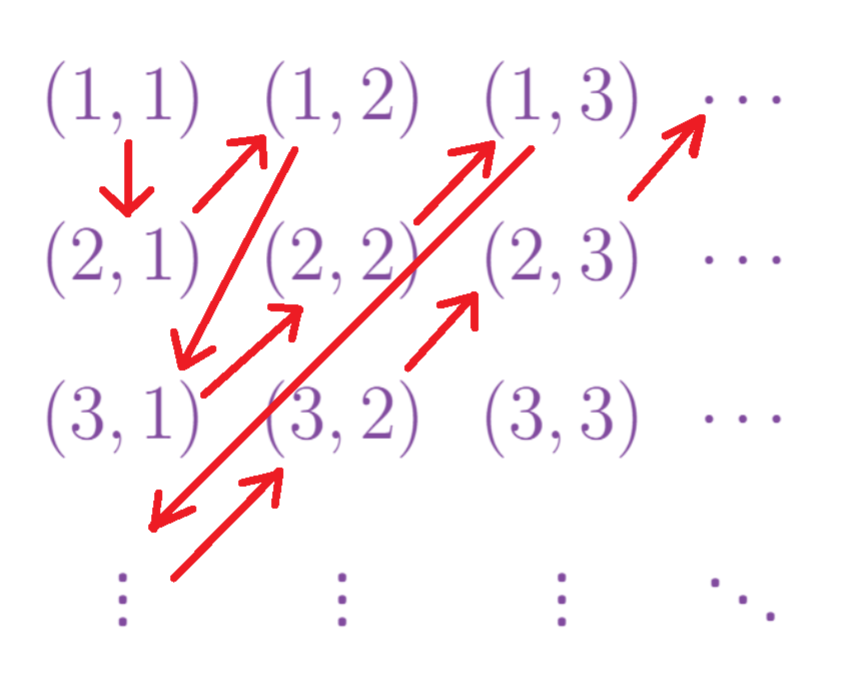
\includegraphics[scale=0.55]{Cartesian_Product_Bijection.png}
      \end{myClosureOneDeprecated}
   \end{center}}
   \retTwo
   \markLecture{1/24/2024}

   {\hTwo
   \begin{myIndent}
      Proposition \propCount: If $A$ is a countable set, $B$ any set, and $g: A\rightarrow B$ is a surjection, then $B$ is countable.
      
      {\begin{myIndent} \hThree
         Proof:\\
         If $A$ is finite, then $B = g(A)$ is finite as well. So the proposition is trivially true. Now assume $A$ is infinite. Then since $A$ is countable, there is a bijection\\ $f: \mathbb{Z}^+ \rightarrow A$. Now define $\phi = g \circ f: \mathbb{Z}^+ \rightarrow B$. We know that $\phi$ is a surjection as it is the composition of two surjections. \retTwo

         Let $E \subseteq \mathbb{Z}^+$ be any set that contains precisely one element of $\phi^{-1}(b)$ for each $b\in B$. For instance, we can define $E$ as the set: \[\{n \in \mathbb{Z}^+ \mid \forall m \in \mathbb{Z}^+, \hspace{0.25em} m<n \Rightarrow \phi(m) \neq \phi(n)\}\]

         \newpage

         Now by proposition 8, we know that $E$ is countable as $E$ is a subset of a \\countable set. But additionally we have that $\phi$ acts as a bijection from $E$ to $B$. Therefore, $\lvert E \rvert = \lvert B \rvert$, meaning $B$ is countable. \retTwo
      \end{myIndent}}

      Proposition \propCount: A set $A$ is countable if and only if there exists a surjection from\\ $\mathbb{Z}^+$ onto $A$.
      {\hThree
      \begin{myIndent}
         Proof:\\
         ($\Longleftarrow$) Since $\mathbb{Z}^+$ is the definition of a countable set, if there is a surjection from $\mathbb{Z}^+$ to $A$, then we have by proposition 10 that $A$ is also countable. \retTwo

         ($\Longrightarrow$) Assume $A$ is countable. If $A$ is finite, then we can number the elements of $A$ as $\{a_1, a_2, \ldots, a_n\}$. So, we may define the surjection $f: \mathbb{Z}^+ \rightarrow A$ with the correspondance rule:
         \[f(k) = \left\{
         \begin{matrix}
            a_k \quad \text{ if } k \leq n \\
            a_n \quad \text{ if } k > n
         \end{matrix}\right.\]
         Meanwhile if $A$ is infinite, then by definition there exists a bijection from $\mathbb{Z}^+$ to $A$. So, no matter if $A$ is infinite or finite, if $A$ is countable, then there exists a bijection from $\mathbb{Z}^+$ to $A$. \retTwo
      \end{myIndent}}

      Proposition \propCount: If $E_n$ is a countable set for each $n\in\mathbb{Z}^+$, then ${\displaystyle \mathlarger{\bigcup}_{\phantom{+}n \in \mathbb{Z}^+}{E_n}}$ is countable.
      
      {\begin{myIndent} \hThree
         Proof:\\ For each $n \in \mathbb{Z}^+$, there is a surjection $f_n: \mathbb{Z}^+ \rightarrow E_n$.\\  Define $g: \mathbb{Z}^+ \times \mathbb{Z}^+ \rightarrow {\displaystyle \mathlarger{\bigcup}_{\phantom{+}n \in \mathbb{Z}^+}{E_n}} \hspace{0.1em}$ by $g(n, k) = f_n(k)$. \retTwo Then as $g$ is a surjection and $\mathbb{Z} \times \mathbb{Z}$ is countable by proposition 9, we know by proposition 10 that ${\displaystyle \mathlarger{\bigcup}_{\phantom{+}n \in \mathbb{Z}^+}{E_n}}$ is countable.
         {\begin{myTindent}\begin{myDindent} \teachComment
            In other words, the union of countably many \\countable sets is countable. \retTwo
         \end{myDindent}\end{myTindent}}
      \end{myIndent}}
      
      Proposition \propCount: If $A$ is countable, then for every $n \in \mathbb{Z}^+$, the set $A^n = A \times A \times \ldots \times A$ is countable.

      {\hThree
      \begin{myIndent}
         Proof: (we can proceed by induction) \\
         When $n=1$, then $A^n = A^1 = A$ is obviously countable.\\
         Now assume the proposition is true for $n-1$, meaning $A^{n-1}$ is countable. Then: $A^n = {\displaystyle \mathlarger{\bigcup}_{a \in A}{\{a\} \times A^{n-1}}}$ is countable by proposition 12.
      \end{myIndent}}
      \newpage

      Corollary: $\mathbb{Q}$ is countable.
      {\begin{myIndent} \hThree
         Proof:\\
         Define $f: \mathbb{Q} \rightarrow \mathbb{Z} \times \mathbb{Z}^+$ by setting $f(p) = (n, m)$ where $n, m$ are the unique coprime integers with $m>0$, $\frac{n}{m}=p$. Also define $f(0) = (1, 0)$ Then\\ $f(\mathbb{Q}) \subset \mathbb{Z} \times \mathbb{Z}^+$ and the latter set is countable. So $f(\mathbb{Q})$ is countable. Since $f$ is injective, $f$ is a bijection between $\mathbb{Q}$ and a countable set. Thus $\mathbb{Q}$ is countable. \retTwo
      \end{myIndent}}
   \end{myIndent}}
   Given sets $A$ and $B$, we write $A^B$ to denote the set of all functions from $B$ to $A$. \retTwo
   
   {\begin{myIndent} \hTwo
      Proposition \propCount: $\{0, 1\}^{\mathbb{Z}^+}$ is uncountable.
      \hThree
      \begin{myIndent}
         Proof: Let $\{f_1, f_2, \ldots\}$ be any countable subset of $\{0, 1\}^{\mathbb{Z}^+}$. Then define\\ $g \in \{0, 1\}^{\mathbb{Z}^+}$ by the rule $g(n) = 1 - f_n(n)$. Since $g(n) \neq f_n(n)$, we have that $g \neq f_n$. Since this holds for all $n \in \mathbb{Z}^+$, we can thus conclude that $g \notin \{f_1, f_2, \ldots\}$. We thus conclude that any countable subset of $\{0, 1\}^{\mathbb{Z}^+}$ is a proper subset. So $\{0, 1\}^{\mathbb{Z}^+}$ must be uncountable.
      \end{myIndent} \retTwo
   \end{myIndent}}

   \markLecture{1/26/2024}

   A \udefine{metric space} is a set $X$ equipped with a function $d: X\times X \longrightarrow \left[0, \infty\right)$ satisfying:
   \begin{enumerate}
      \item $\forall p, q \in X \quad p\neq q \Rightarrow d(p, q) > 0$ whereas $p=q \Rightarrow d(p, q) = 0$
      \item $\forall p, q \in X \quad d(p, q)=d(q, p)$
      \item $\forall p, q, s \in X \quad d(p, q) \leq d(p, s) + d(s, q)$
   \end{enumerate} \retTwo

   The function $d$ is called a distance function or \udefine{metric}.
   {\hTwo
   \begin{myIndent}
      Examples:
      \begin{itemize}
         \item $\mathbb{R}^k$ is a metric space (we have several metrics to choose from):
         {\hThree
         \begin{itemize}
            \item[\diamond] $d_p(\mVec{x}, \mVec{y}) = \left(\sum{\left| x_i - y_i\right|^p}\right)^\frac{1}{p}$
            {\begin{myTindent} \teachComment
               $d_2(\mVec{x}, \mVec{y})=\| \mVec{x} - \mVec{y} \|$
            \end{myTindent}}
            \item[\diamond] $d_\infty(\mVec{x}, \mVec{y}) = \max\limits_{1\leq i \leq k}{\lvert x_i - y_i \rvert}$
         \end{itemize}}

         \item Any set $X$ is a metric space when equipped with the \udefine{discrete metric}:
         {\begin{myIndent} \hThree
            $d(p, q) = \left\{ \begin{matrix} 0 \text{ if } p=q\\ 1 \text{ if } p\neq q \end{matrix} \right.$
         \end{myIndent}}

         \item The set of all functions from $[0, 1] \rightarrow [0, 1]$ can be equipped with the metric: \hThree
         \begin{myIndent}
            $d(f, g) = \sup\limits_{x\in[0, 1]}{\left| f(x)-g(x) \right|}$
         \end{myIndent} \retTwo
      \end{itemize}
   \end{myIndent}}

   \newpage
   Let $X$ be a metric space. Then for $p \in X$ and $r > 0$, the (open) \udefine{ball} of radius $r$ around $p$ is $B_r(p) = \{q \in X \mid d(p, q)<r\}$. \retTwo
   
   {\begin{myIndent} \hTwo
      $p \in X$ is a \udefine{limit point} of $E \subseteq X$ if there are points in $E \setminus \{p\}$ that are arbitrarily close to $p$. Or in other words, if $p$ is a limit point, then
   
      {\centering $\forall r>0, \quad ((B_r(p) \setminus \{p\}) \cap E) \neq \emptyset$.\retTwo \par}
   
      The set of limit points of $E \subseteq X$ is denoted $E^\prime$.
      \begin{itemize}
         \item $E$ is \udefine{closed} if $E^\prime \subseteq E$.
         \item $E$ is \udefine{perfect} if $E = E^\prime$.
         \item We say $E$ is \udefine{dense} in $X$ if $E \cup E^\prime = X$
      \end{itemize} \retTwo \retTwo
   
      $p \in X$ is an \udefine{interior point} of $E \subseteq X$ if $\exists r > 0 \suchthat B_r(p) \subseteq E$. \retTwo
   
      The set of interior points of $E$ is denoted $E^\circ$.
      \begin{itemize}
         \item $E$ is \udefine{open} if $E^\circ = E$.
         \item $E$ is a \udefine{neighborhood} of $p$ if $p \in E^\circ$.
      \end{itemize} \retTwo \retTwo
   
      The \udefine{complement} of $E$ is $E^\comp = X \setminus E$. \\
      $E$ is \udefine{bounded} if there is a point $p \in X$ and $R > 0$ with $E \subseteq B_R(p)$. \\
      If $p \in E$, we say $p$ is an \udefine{isolated} point of $E$ if $\exists r>0 \suchthat B_r(p)\cap E = \{p\}$.
   \end{myIndent}}

   \mySepTwo

   {\begin{myIndent} \hTwo
      Proposition \propCount: If $X$ is a metric space, $p \in X$, and $r > 0$, then $B_r(p)$ is open.
      {\hThree
      \begin{myIndent}
         Proof:\\
         Consider a point $q \in B_r(p)$. We claim that $B_{(r-d(p, q))}(q) \subseteq B_r(p)$.\\ To prove this consider that for $z \in B_{(r-d(p, q))}(q)$, we have that\\ $d(p, z) \leq d(p, q) + d(q, z) < d(p, q) + (r - d(p, q)) = r$. Thus, $z \in B_r(p)$. And, since we can do this for any $z \in B_{(r-d(p, q))}(q)$, we know that\\ $B_{(r-d(p, q))}(q) \subseteq B_r(p)$. Therefore $q$ is an interior point of $B_r(p)$. And, since we can say this for any $q \in B_r(p)$, we thus conclude that $B_r(p)$ consists of interior points. So $B_r(p)$ is open.
      \end{myIndent}}
   \end{myIndent}}
   \newpage
   \markLecture{1/29/2024}

   Let $X$ be a metric with metric $d$ and let $E \subseteq X$\dots \retTwo
   {\begin{myIndent} \hTwo
      Proposition \propCount: If $p \in E^\prime$, then $(B_r(p) \setminus \{p\}) \cap E$ is infinite for every $r > 0$.
      
      {\begin{myIndent} \hThree
         Proof (by contrapositive):\\
         Let $p \in X$ and suppose $\exists r > 0$ with $(B_r(p) \setminus \{p\}) \cap E$ finite.\\ Then set $t = \min{\{d(p, q) \mid q \in (B_r(p) \setminus \{p\}) \cap E\}}$. That way, we must have that $t>0$.
         But at the same time, $B_t(p) \setminus \{p\} \cap E$ is empty. Therefore $p \notin E^\prime$. \retTwo
      \end{myIndent}}

      Corollary: If $E$ is finite, then $E^\prime = \emptyset$. This means that finite sets are always closed. \retTwo

      Propostion \propCount: $E$ is open if and only if $E^\comp$ is closed.

      {\begin{myIndent} \hThree
         Proof:\\
         \begin{tabular}{ r c l }
            $E^\comp$ is closed & $\Longleftrightarrow$ & $\left(E^\comp\right)^\prime \subseteq E^\comp$ \\
            & $\Longleftrightarrow$ & $\left(E^C\right)^\prime \cap E = \emptyset$ \\
            & $\Longleftrightarrow$ & $\forall p \in E, \hspace{0.5em} p \notin \left(E^\comp\right)^\prime$ \\
            & $\Longleftrightarrow$ & $\forall p \in E, \hspace{0.5em} \exists r > 0 \suchthat (B_r(p) \setminus \{p\}) \cap E^\comp = \emptyset$ \\
            & $\Longleftrightarrow$ & $\forall p \in E, \hspace{0.5em} \exists r > 0 \suchthat B_r(p) \setminus \{p\} \subseteq E$ \\
            & $\Longleftrightarrow$ & $\forall p \in E, \hspace{0.5em} \exists r > 0 \suchthat B_r(p) \subseteq E$ \\
            & $\Longleftrightarrow$ & $\forall p \in E, \hspace{0.5em} p \in E^\circ$\\
            & $\Longleftrightarrow$ & $E$ is open\\
         \end{tabular} \retTwo
      \end{myIndent}}

      Corollary: $E$ is closed if and only if $E^\comp$ is open. \retTwo

      Proposition \propCount: Let $A$ be any set.
      \begin{enumerate}
         \item If $u_\alpha \subseteq X$ is an open set for each $\alpha \in A$, then ${\displaystyle \bigcup_{\alpha \in A}{u_\alpha}}$ is open.
         
         {\begin{myIndent} \hThree
            Proof:\\ Let $p \in {\displaystyle \bigcup_{\alpha \in A}{u_\alpha}}$. Pick $\beta \in A$ with $p \in u_\beta$.\\
            Since $u_\beta$ is open, we know that $\exists r>0 \suchthat B_r(p) \subseteq u_\beta \subseteq {\displaystyle \bigcup_{\alpha \in A}{u_\alpha}}$.\\ So $p$ is an interior point. Hence, we conclude that ${\displaystyle \bigcup_{\alpha \in A}{u_\alpha}}$ is open. \retTwo
         \end{myIndent}}

         \item If $F_\alpha \subseteq X$ is a closed set for each $\alpha \in A$, then  ${\displaystyle \bigcap_{\alpha \in A}{F_\alpha}}$ is closed.
         
         {\begin{myIndent} \hThree
            Proof:\\ $\left({\displaystyle \bigcap_{\alpha \in A}{F_\alpha}}\right)^\comp = {\displaystyle \bigcup_{\alpha \in A}{\left(F_\alpha\right)^\comp}}$ by De Morgan's laws.
            \newpage
            Since each $F_\alpha$ is closed, we know each $\left(F_\alpha\right)^\comp$ is open.\\ So by proposition 18.1, we know that ${\displaystyle \bigcup_{\alpha \in A}{\left(F_\alpha\right)^\comp}}$ is open.\\ Then, by proposition 17, we know that its complement, ${\displaystyle \bigcap_{\alpha \in A}{F_\alpha}}$ is closed. \retTwo
         \end{myIndent}}

         \item If $u_1, u_2, \ldots, u_n \subseteq X$ are open, then ${\displaystyle \bigcap_{i = 1}^n{u_i}}$ is open.
         

         {\begin{myIndent} \hThree
            Proof:\\
            Let $p \in {\displaystyle \bigcap_{i = 1}^n{u_i}}$. Then $p \in u_i$ for every $i$.\\
            Since $u_i$ is open, $\exists r_i > 0 \suchthat B_{r_i}(p) \subseteq u_i$. Therefore, set\\ $r = \min{\{r_i \mid 1\leq i \leq n\}}$ so that for all $i$, $B_r(p) \subseteq B_{r_i}(p) \subseteq u_i$.\\
            Hence, $B_r(p) \subseteq {\displaystyle \bigcap_{i = 1}^n{u_i}}$. We thus conclude that ${\displaystyle \bigcap_{i = 1}^n{u_i}}$ is open. \retTwo
         \end{myIndent}}

         \item If $F_1, F_2, \ldots, F_n \subseteq X$ are closed, then ${\displaystyle \bigcup_{i = 1}^n{F_i}}$ is closed.
         

         {\begin{myIndent} \hThree
            The proof of this follows from proposition 18.3 in the same way that proposition 18.2 follows from proposition 18.1. \retTwo
         \end{myIndent}}
      \end{enumerate}
   \end{myIndent}}

   \markLecture{2/2/2024}

   Given a metric space $X$, the \udefine{closure} of $E \subseteq X$ is $\overbar*{E}\coloneq E \cup E^\prime$. \retTwo

   {\begin{myIndent} \hTwo
      \resetSubPropCount
      Proposition \propCount.\subPropCount: $\overbar{E}$ is closed.

      {\begin{myIndent} \hThree
         Proof:\\
         Let $p \in (\myBar{E})^\comp$. Thus, $p \notin E^\prime$, meaning that we can fix $r>0$ so that\\ $(B_r(p) \setminus \{p\}) \cap E = \emptyset$. Additionally, since $p \notin E$, we have that $B_r(p) \cap E = \emptyset$. \retTwo

         Now consider any $q \in B_r(p)$. Setting $t = r - d(p, q)$, we have that\\ $B_t(q) \subseteq B_r(p)$. Therefore, since $B_r(p) \cap E = \emptyset$, we know $B_t(q) \cap E = \emptyset$. This tells us that $q \notin E^\prime$. Hence, $B_r(p) \cap E^\prime = \emptyset$.
         \retTwo

         We've now shown that $B_r(p) \cap E = \emptyset$ and that $B_r(p) \cap E^\prime = \emptyset$.\\ Therefore, $B_r(p) \cap (E \cup E^\prime) = B_r(p) \cap \overbar{E} = \emptyset$, meaning that $B_r(p) \subseteq (\overbar{E})^\comp$. So $(\overbar{E})^\comp$ is open, meaning that $\overbar{E}$ is closed.
      \end{myIndent}}

      \newpage

      Proposition \propCount[0].\subPropCount: $E = \overbar{E}$ if and only if $E$ is closed.

      {\begin{myIndent} \hThree
         Proof:\\
         ($\Longrightarrow$) If $\overbar{E}$ is closed by proposition 19.1. So $E = \overbar{E}$ implies $E$ is closed.\\
         ($\Longleftarrow$) If $E$ is closed, then $E^\prime \subseteq E$. Hence, $\overbar{E} = E \cup E^\prime = E$ \retTwo
      \end{myIndent}}

      Proposition \propCount[0].\subPropCount: If $F$ is closed and $F \supseteq E$, then $F \supseteq \overbar{E}$.

      {\begin{myIndent} \hThree
         Proof:\\
         Observe that if $F$ is any set and $E \subseteq F$, then $E^\prime \subseteq F^\prime$. Thus, if $F$ is also closed, we have that $E^\prime \subseteq F^\prime \subseteq F$. Therefore, $F = F \cup F^\prime \supseteq E \cup E^\prime = \myBar{E}$.
         \retTwo
      \end{myIndent}}
   \end{myIndent}}

   \mySepTwo

   Note that in this class, unless it is mentioned otherwise, you should assume that we are equipping $\mathbb{R}$ or $\mathbb{R}^k$ with the \udefine{Euclidean} metric: $d_2$.

   {\begin{myIndent} \hTwo
      Proposition \propCount: If $E \subseteq \mathbb{R}$ is nonempty and bounded above, then $\sup{E} \in \overbar{E}$.

      {\begin{myIndent} \hThree
         Proof:\\
         Set $y = \sup{E}$. If $y \in E$, then we are done. So assume $y \notin E$.\\
         Consider any $r > 0$. Since $y - r < y = \sup{E}$, we know $y-r$ is not an upperbound to $E$. Hence, there is $e \in E$ with $y-r<e<y$. Therefore, $(B_r(y) \setminus \{y\}) \cap E \neq \emptyset$. Hence, we conclude that $y \in E^\prime \subseteq \overbar{E}$. \retTwo
      \end{myIndent}}
   \end{myIndent}}

   \mySepTwo

   Note that if $X$ is a metric space with metric $d$ and $Y \subseteq X$, then $Y$ is also a metric space with $d$ when $d$ is restricted to $Y$. \retTwo
   $E \subseteq Y \subseteq X$ is \udefine{open/closed/etc. relative to $Y$} if $E$ is open/closed/etc. in the metric space $Y$. \retTwo

   {\begin{myIndent} \hTwo
      If $Y \subseteq X$ and $B_r(p)$ denotes the ball of radius $r$ around $p \in Y$ in the metric space $X$, then the ball of radius $r$ around $p$ in the metric space $Y$ is $B_r(p) \cap Y$. \retTwo

      Proposition \propCount: Let $E \subseteq Y \subseteq X$. Then $E$ is open relative to $Y$ if and only if there is an open set $U \subseteq X$ with $E = U \cap Y$.

      {\begin{myIndent} \hThree
         Proof:\\
         ($\Longrightarrow$) For each $p \in E$, pick $r(p) > 0$ so that $B_{r(p)}(p) \cap Y \subseteq E$. Then, setting $U = {\displaystyle \bigcup_{p\in E}{B_{r(p)}(p)}}$, we have that $U$ is open and that \[E = \bigcup_{p\in E}{\{p\}} \subseteq \bigcup_{p\in E}{B_{r(p)}(p)} \cap Y = U \cap Y \subseteq E\]
         So $U \cap Y = E$. \retTwo

         ($\Longleftarrow$) Now say that $E = U \cap Y$ where $U \subseteq X$ is open. Also let $p \in E$.\\ We know $p \in U$. Additionally, since $U$ is open, there is $r > 0$ with $B_r(p) \subseteq U$. Consequently, $B_r(p) \cap Y \subseteq U \cap Y = E$. So, $p$ is an interior point of $E$ relative to $Y$. We conclude that $E$ is open relative to $Y$. \retTwo
      \end{myIndent}}
   \end{myIndent}}
   
   \mySepTwo

   Let $X$ be a metric space. An \udefine{open cover} of $E \subseteq X$ is a collection $\{u_\alpha \mid \alpha \in A\}$ of open sets $u_\alpha$ satisfying:

   {\centering $ E \subseteq {\displaystyle \bigcup_{\alpha \in A}{u_\alpha}}$\retTwo \par}

   $K \subseteq X$ is \udefine{compact} if every open cover of $K$ containsa finite subcover of $K$.
   {\begin{myIndent} \hTwo
      More precisely: $K$ is compact if and only if for ever open cover $\{u_\alpha \mid \alpha \in A\}$ of $K$, there is $n \in \mathbb{Z}^+$ and $\alpha_1, \alpha_2, \ldots, \alpha_n \in A$ such that:

      
      {\centering $ K \subseteq {\displaystyle \bigcup_{i = 1}^n{u_{\alpha_i}}}$\retTwo \par}

      
      {\begin{myTindent}\begin{myTindent}\begin{myIndent} \teachComment
         As an aside, compactness often acts as a\\ generalization of finiteness in topology.
      \end{myIndent}\end{myTindent}\end{myTindent}}
   \end{myIndent}}

   \markLecture{2/5/2024}

   {\begin{myIndent} \hTwo
      Finite sets are compact. \retTwo
      Proposition \propCount: compactness is an \uuline{intrinisic} property, meaning if $K \subseteq Y \subseteq X$,\\ then $K$ is compact relative to $X$ if and only if $K$ is compact relative to $Y$.
      
      {\begin{myIndent} \hThree
         Proof:\\
         ($\Longrightarrow$) Consider any collection of sets $v_\alpha \subseteq Y$ that are open relative to $Y$ and satisfy that $K \subseteq {\displaystyle \bigcup_{\alpha \in A}{v_\alpha}}$. \retTwo
         By a previous theorem, we know there are sets $w_\alpha$  open relative to $X$ such that $v_\alpha = w_\alpha \cap Y$. So we have that $K \subseteq {\displaystyle \bigcup_{\alpha \in A}{v_\alpha}} \subseteq {\displaystyle \bigcup_{\alpha \in A}{w_\alpha}}$. \retTwo
         If $K$ is compact relative to $X$, then there exists $n \in \mathbb{Z}^+$ and $\alpha_1, \ldots, \alpha_n \in A$ such that $K \subseteq {\displaystyle \bigcup^n_{i=1}{w_{\alpha_i}}}$. And since $K \subseteq Y$, we have that:
         \[K = K \cap Y \subseteq \left(\bigcup^n_{i=1}{w_{\alpha_i}}\right)\cap Y = \left(\bigcup^n_{i=1}{v_{\alpha_i}}\right)\]
         Hence, $K$ is compact relative to $Y$.

         \newpage

         ($\Longleftarrow$) Now consider any set $K$ which is compact relative to $Y$ and open cover\\ $\{w_\alpha \mid \alpha \in A\}$ such that $w_\alpha \subseteq X$ and $K \subseteq {\displaystyle \bigcup_{\alpha \in A}{w_\alpha}}$. \retTwo By proposition 21, we know that $v_\alpha = w_\alpha \cap Y$ is open relative to $Y$. So as\\ $K \subseteq Y$, we have that $K = K \cap Y \subseteq {\displaystyle \bigcup_{\alpha \in A}{w_\alpha}} \cap Y = {\displaystyle \bigcup_{\alpha \in A}{v_\alpha}}$. \retTwo But that means that $\{v_\alpha \mid \alpha \in A\}$ forms an open cover of $K$ relative to $Y$. So, there exists $n \in \mathbb{Z}^+$ and $\alpha_1, \ldots, \alpha_n \in A$ such that $\{v_{\alpha_1}, \ldots, v_{\alpha_n}\}$ is a finite cover of $K$. Then note that:
         \[K \subseteq \bigcup^n_{i=1}{v_{\alpha_i}} \subseteq \bigcup^n_{i=1}{w_{\alpha_i}}\]
         So, $\{w_{\alpha_1}, \ldots, w_{\alpha_n}\}$ forms a finite subcover of $K$ using sets in our original arbitrary open cover. Therefore, we conclude that $K$ is compact relative to $X$. \retTwo
      \end{myIndent}}

      Proposition \propCount: Compact sets are closed.

      {\begin{myIndent} \hThree
         Proof:\\
         Let $K \subseteq X$ be compact. It then suffices to show that $K^\comp$ is open. So, consider any $p \in K^\comp$. We know that $\{B_{\frac{1}{3}d(p, q)}(q) \mid q \in K\}$ forms an open cover of $K$. Additionally, because $K$ is compact, there exists $n \in \mathbb{Z}^+$ and $q_1, \ldots, q_n \in K$ such that:
         \[K \subseteq \bigcup_{i=1}^n{B_{\frac{1}{3}d(p, q_i)}(q_i)}\]
         Thus, let $r = \min{\{d(p, q_i) \mid 1 \leq i \leq n\}}$. That way, $\frac{1}{3}r > 0$ and \[\left(\bigcup_{i=1}^n{B_{\frac{1}{3}d(p, q_i)}(q_i)} \right) \cap B_{\frac{1}{3}r}(p) = \emptyset\text{.}\]
         This then means that $K \cap B_{\frac{1}{3}r}(p) = \emptyset$, meaning that $B_{\frac{1}{3}r}(p) \subseteq K^\comp$. So $p$ is an interior point of $K^\comp$. We thus conclude that $K^\comp$ is open. \retTwo
      \end{myIndent}}
      
      Proposition \propCount: $K$ is compact and $F \subseteq K$ is closed implies that $F$ is compact.
      
      {\begin{myIndent} \hThree
         Proof:\\
         Consider any open cover $\{v_\alpha \mid \alpha \in A\}$ of $F$. Since $F$ is closed, $F^\comp$ is open. So, we can say that $\{F^\comp\} \cup \{v_\alpha \mid \alpha \in A\}$ is an open cover of $K$ as: \[\left(\bigcup_{\alpha \in A}{v_\alpha}\right) \cup F^\comp \supseteq F \cup F^\comp \supseteq K\] 
         \newpage
         Since $K$ is compact, there exists $n \in \mathbb{Z}^+$ and $\alpha_1, \ldots, \alpha_n \in A$ such that: \[K \subseteq \left(\bigcup_{i=1}^n{v_{\alpha_i}}\right) \cup F^\comp\]
         {\begin{myTindent} \teachComment
            $F^\comp$ may or may not be needed to cover $K$. However, its \\inclusion doesn't effect the finiteness of the cover. \retTwo
         \end{myTindent}}
         Therefore $F \subseteq {\displaystyle \bigcup_{i=1}^n{v_{\alpha_i}}}$. So, $F$ is compact. \retTwo
      \end{myIndent}}

      Corollary: $K$ is compact and $F$ is closed implies that $K \cap F$ is compact.
      {\begin{myIndent} \hThree
         Proof: $K$ being compact means that $K$ is closed. Thus $K \cap F$ is closed. And as $K \cap F$ is a subset of $K$, by the above theorem we have that $K \cap F$ is compact.
         \retTwo
      \end{myIndent}}

      \uuline{Theorem (the Finite Intersection Property)}: If $\{K_\alpha \mid \alpha \in A\}$ is any collection of compact sets in $X$ having the property that the intersection of any finitely many of the $K_\alpha$'s is nonempty, then: \[\bigcap_{\alpha \in A}{K_\alpha} \neq \emptyset\]

      {\begin{myIndent} \hThree
         Proof: (we shall proceed by proving the contrapositive...)\\
         Assume that ${\displaystyle \bigcap_{\alpha \in A}{K_\alpha} = \emptyset}$. Thus, taking complements gives: ${\displaystyle \bigcup_{\alpha \in A}{(X \setminus K_\alpha)}} = X$. \retTwo
         Pick any $\alpha_0 \in A$. Then $\{X \setminus K_\alpha \mid \alpha \in A\}$ is an open cover of $K_{\alpha_0}$ because $K_{\alpha_0} \subseteq X$ and because each $X \setminus K_\alpha$ must be open due to $K_\alpha$ being closed. \retTwo
         As $K_{\alpha_0}$ is compact, there exists $n \in \mathbb{Z}^+$ and $\alpha_1, \ldots, \alpha_n \in A$ such that: \[K_{\alpha_0} \subseteq \bigcup_{i=1}^n{(X \setminus K_{\alpha_i})}\]
         Taking complements again, we get that: $X \setminus K_{\alpha_0} \supseteq {\displaystyle \bigcap_{i=1}^n{(K_{\alpha_i})}}$. So: \[\left(\bigcap_{i=1}^n{(K_{\alpha_i})}\right) \cap K_{\alpha_0} = \bigcap_{i=0}^n{(K_{\alpha_i})} = \emptyset\]
      \end{myIndent}}

      \newpage

      Proposition \propCount: If $K$ is compact and $E \subseteq K$ is infinite, then $E^\prime \neq \emptyset$.

      {\begin{myIndent} \hThree
         Proof: (we shall proceed by proving the contrapositive...)\\
         Let $E \subseteq K$ and suppose $E^\prime = \emptyset$. Then for each $q \in K$, since $q \notin E^\prime$, we can pick $r(q) > 0$ such that $(B_{r(q)}(q) \setminus \{q\}) \cap E = \emptyset$. In particular,\\ $(B_{r(q)}(q)) \cap E \subseteq \{q\}$. \retTwo

         Now note that ${\displaystyle \bigcup_{q \in K}{B_{r(q)}(q)}}$ is an open cover of $K$.\\ Since $K$ is compact, we can pick $q_1, \ldots, q_n \in K$ so that $K \subseteq {\displaystyle \bigcup_{i=1}^n{B_{r(q_i)}(q_i)}}$.\\

         Then, $E = E \cap K \subseteq E \cap \left({\displaystyle \bigcup_{i=1}^n{B_{r(q_i)}(q_i)}}\right) = {\displaystyle \bigcup_{i=1}^n{\left(B_{r(q_i)}(q_i) \cap E\right)}} \subseteq {\displaystyle \bigcup_{i=1}^n{q_i}}$. \\

         Hence $E$ is finite.
      \end{myIndent}}
   \end{myIndent}}

   \retTwo
   \markLecture{2/7/2024} \retTwo
   In $\mathbb{R}$, we define the \udefine{interval} $[a, b] = \{x \in \mathbb{R} \mid a \leq x \leq b\}$.

   {\begin{myIndent} \hTwo
      Proposition \propCount: If $I_n = [a_n, b_n] \neq \emptyset$ and $I_{n+1} \subseteq I_n$ for all $n$, then ${\displaystyle \bigcap_{n\in\mathbb{N}}{I_n} \neq \emptyset}$. \\

      {\begin{myIndent} \hThree
         Proof: For all $n, m \in \mathbb{N}$, we have $a_n \leq a_{n+m} \leq b_{n+m} \leq b_m$. Thus, for all $m$ we have that $b_m$ is an upperbound to $\{a_n \mid n\in\mathbb{N}\}$. This means that by the least upper bound property of $\mathbb{R}$, we know that $\alpha = \sup{\{a_n \mid n\in\mathbb{N}\}}$ exists and that $a_m \leq \alpha \leq b_m$ for all $m$. Hence, $\alpha \in {\displaystyle \bigcap_{n \in \mathbb{N}}{I_n}}$, which means ${\displaystyle \bigcap_{n \in \mathbb{N}}{I_n}} \neq \emptyset$.\retTwo
      \end{myIndent}}

      Corollary: If $C_n = [a_{n, 1}, b_{n, 1}] \times [a_{n, 2}, b_{n, 2}] \times \dots \times [a_{n, k}, b_{n, k}] \subseteq \mathbb{R}^k$ and $C_{n+1} \subseteq C_n$ for all $n \in \mathbb{N}$, then ${\displaystyle \bigcap_{n\in\mathbb{N}}{C_n} \neq \emptyset}$.

      {\begin{myIndent} \hThree
         Proof: $\quad {\displaystyle \bigcap_{n\in\mathbb{N}}{C_n} = \left(\bigcap_{n\in\mathbb{N}}{[a_{n, 1}, b_{n, 1}]}\right) \times \dots \times \left(\bigcap_{n\in\mathbb{N}}{[a_{n, 1}, b_{n, 1}]}\right) \neq \emptyset}$
         \retTwo \retTwo
      \end{myIndent}}

      \newpage

      Proposition \propCount: $C = [a_{1}, b_{1}] \times [a_{2}, b_{2}] \times \dots \times [a_{k}, b_{k}] \subseteq \mathbb{R}^k$ is compact.

      \begin{myIndent} \hThree
         Proof: (we'll proceed by finding a contradiction)
         Suppose $\{u_\alpha \mid \alpha \in A\}$ is an open cover of $C$ containing no finite subcover of $C$. \retTwo Then set $\delta = \sqrt{{\displaystyle \sum_{i=1}^k{b_i - a_i}}}$
         
         {\begin{myTindent}\begin{myIndent} \hFour
            (this is the length of the largest diagonal of $C$.) \retTwo
         \end{myIndent}\end{myTindent}}

         Since $C$ forms a $k$-dimensional rectangle in $\mathbb{R}^k$, we can divide $C$ into $2^k$ many pieces by cutting each side of $C$ at its midpoints. Then each smaller piece will have a longest diagonal of length $\frac{1}{2}\delta$. \newline
         {\center \raisebox{0em}{\tikz[scale=0.5]{
            \draw[color=Red, very thick ,dashed] (0, 0) -- (8, 5);
            \draw[color=Purple, ultra thick] (0, 0) rectangle (8, 5);
            \draw[color=RedViolet, very thick] (0, 2.5) -- (8, 2.5);
            \draw[color=RedViolet, very thick] (4, 0) -- (4, 5);
         }} \retTwo\par}

         Since $C$ can't be covered by finitely many $u_\alpha$, there must be a piece, call it $C_1$, which cannot be covered by finitely many $u_\alpha$. Also $C_1 \subseteq C$. \retTwo

         Now proceed inductively to build a sequence $C_n$ such that:
         \begin{enumerate}
            \item $C_{n+1} \subset C_n$ for all $n$
            \item The largest diagonal of $C_n$ is $2^{-n}\delta$
            \item $C_n$ cannot be covered by finitely many $u_\alpha$ \newline
         \end{enumerate}
         {\center \raisebox{0em}{\tikz[scale=0.5]{
            \draw[color=Red, very thick ,dashed] (0, 0) -- (8, 5);
            \draw[color=Purple, ultra thick] (0, 0) rectangle (8, 5);
            % C1
            \draw[color=RedViolet, very thick] (0, 2.5) -- (8, 2.5);
            \draw[color=RedViolet, very thick] (4, 0) -- (4, 5);
            % C2
            \draw[color=RedViolet, thick] (0, 3.75) -- (4, 3.75);
            \draw[color=RedViolet, thick] (2, 2.5) -- (2, 5);
            % C3
            \draw[color=RedViolet, semithick] (2, 3.125) -- (4, 3.125);
            \draw[color=RedViolet, semithick] (3, 2.5) -- (3, 3.75);
            % C4
            \draw[color=RedViolet, thin] (2, 2.8125) -- (3, 2.8125);
            \draw[color=RedViolet, thin] (2.5, 2.5) -- (2.5, 3.125);
            % C5
            \draw[color=RedViolet, thin] (2, 2.96875) -- (2.5, 2.96875);
            \draw[color=RedViolet, thin] (2.25, 2.8125) -- (2.25, 3.125);
            % C6
            \draw[color=RedViolet, very thin] (2.25, 2.890625) -- (2.5, 2.890625);
            \draw[color=RedViolet, very thin] (2.375, 2.8125) -- (2.375, 2.96875);
            % C7
            \draw[color=RedViolet, very thin] (2.375, 2.9296875) -- (2.5, 2.9296875);
            \draw[color=RedViolet, very thin] (2.4375, 2.890625) -- (2.4375, 2.96875);

            %\fill[color=RedViolet] (2.375, 2.890625) rectangle (2.5, 2.96875);
         }} \retTwo\par}

         By the above corollary, ${\displaystyle \bigcap_{n\in\mathbb{N}}{C_n} \neq \emptyset}$. Thus consider $z \in {\displaystyle \bigcap_{n\in\mathbb{N}}{C_n}} \subseteq C$. \\
         Pick $\alpha \in A$ with $z \in u_\alpha$. Since $u_\alpha$ is open, there exists $r > 0$ with $B_r(z) \subseteq u_\alpha$. Now pick $n$ with $2^{-n}\delta < r$. Then as $z \in C_n$, we know $C_n \subseteq B_r(z) \subseteq u_\alpha$. This contradicts the point that $C_n$ cannot be covered by finitely many $u_\alpha$. \retTwo
         So we conclude $C$ is compact. \retTwo
      \end{myIndent}

      \newpage

      Proposition \propCount: For $E \in \mathbb{R}^k$, the following are equivalent:
      \begin{enumerate}
         \item[a.] $E$ is closed and bounded.
         \item[b.] $E$ is compact
         \item[c.] Every infinite subset of $E$ has a limit point in $E$.
      \end{enumerate}

      {\begin{myIndent} \hThree
         Proof: \\
         (a. $\Longrightarrow$ b.) $E$ is bounded means $E \subseteq C$ for some bounded rectangle $C$. Since $E$ is closed and $C$ is compact, $E$ is compact by proposition 24. \retTwo

         (b. $\Longrightarrow$ c.) This is just proposition 25. \retTwo

         (c. $\Longrightarrow$ a.) Firstly, let us show that $E$ is bounded.
         {\begin{myIndent} \hFour
            Suppose $E$ is not bounded. Then for all $n \in \mathbb{N}$, pick $\mVecAst{x}_n \in E$ with $\|\mVecAst{x}_n\|\geq n$.\\
            For any $\mVec{y} \in \mathbb{R}^k$, we have that: $\mVecAst{x}_n \in B_1(\mVec{y}) \Longrightarrow \|\mVecAst{x}_n\| \leq \|\mVec{y}\| + 1$, which in turn implies that $n \leq \|\mVec{y}\| + 1$. So $(B_1(\mVec{y}) \setminus \{\mVec{y}\}) \cap \{\mVecAst{x}_n \mid n \in \mathbb{N}\}$ is finite. As a result, we know $\mVec{y} \notin \{\mVecAst{x}_n \mid n \in \mathbb{N}\}^\prime$. Thus, $\{\mVecAst{x}_n \mid n \in \mathbb{N}\}$ has no limit points. But this is a contradiction because $\{\mVecAst{x}_n \mid n \in \mathbb{N}\}$ is an infinite subset of $E$. \retTwo
         \end{myIndent}}
         Now, let us show that $E$ is closed.
         {\begin{myIndent} \hFour
            Let $y \in E^\prime$. Then for each $n \in \mathbb{Z}^+$, we can pick $\mVecAst{x}_n \in B_{\frac{1}{n}}(\mVec{y}) \cap E$. Now if $\mVec{z} \in \mathbb{R}^k$ and $\mVec{z} \neq \mVec{y}$, then: \retTwo
            
            \begin{myIndent}
               \begin{tabular}{r c l}
                  $\mVecAst{x}_n \in B_{\frac{1}{2}\|\mVec{y}-\mVec{z}\|}(\mVec{z})$&$\Rightarrow$&$\|\mVec{y} - \mVec{z}\| \leq \|\mVec{y} - \mVecAst{x}_n\| + \|\mVecAst{x}_n - \mVec{z}\|$ \\ [0.2em]
                  & & $\phantom{\|\mVec{y} - \mVec{z}\|} < \|\mVec{y} - \mVecAst{x}_n\| + \frac{1}{2}\|\mVecAst{y} - \mVec{z}\|$ \\ [0.6em]
                  & $\Rightarrow$ & $\frac{1}{2}\|\mVecAst{y} - \mVec{z}\| < \|\mVec{y} - \mVecAst{x}_n\| < \frac{1}{n}$ \\ [0.6em]
                  & $\Rightarrow$ & $n < \frac{2}{\|\mVec{y} - \mVecAst{x}_n\|}$
               \end{tabular}
            \end{myIndent}\retTwo

            Therefore: $\left(B_{\frac{1}{2}\|\mVec{y}-\mVec{z}\|}(\mVec{z})\setminus \{\mVec{z}\}\right) \cap \{\mVecAst{x}_n \mid n \in \mathbb{Z}^+\}$ is finite.\\ So $\mVec{z} \notin \{\mVecAst{x}_n \mid n \in \mathbb{N}\}^\prime$, which means that $\mVec{y}$ is the unique limit point of\\ $\{\mVecAst{x}_n \mid n \in \mathbb{N}\}$. Finally, since we assumed that any infinite subset of $E$ has at least one limit point inside $E$, we know that $\mVec{y} \in E$ because it is the only possible limit point that can fulfill this requirement. \retTwo
         \end{myIndent}}
      \end{myIndent}}


      Proposition \propCount: (\uuline{Bolzano-Weierstrauss Theorem}): Every bounded infinite subset of $\mathbb{R}^k$ has a limit point.
      
      {\begin{myIndent} \hThree
         Proof: Let $E$ be a bounded infinite subset of $\mathbb{R}^k$. Then $\overbar{E}$ is closed and bounded, meaning that every infinite subset of $\overbar{E}$ has a limit point in $\overbar{E}$, meaning\\ $(\overbar{E})^\prime \neq \emptyset$. Finally, we know from a homework question last week that\\ $(\overbar{E})^\prime = E^\prime$. So, $E^\prime \neq \emptyset\vphantom{\overbar{E}}$. 
      \end{myIndent}}
   \end{myIndent}}

   \newpage

   The \udefine{Cantor Set} is very important as a counter example in topology. It is constructed as follows:

   \begin{myIndent}
      Let $E_0 = \{[0, 1]\}$. Then for $n > 0$, inductively define $E_n$ as a set containing closed intervals of the first and last thirds of each interval in $E_{n-1}$. \retTwo

      Additionally, for $0 \leq i$, define $C_i = {\displaystyle \bigcup_{I \in E_i}{I}}$. \retTwo

      
      {\begin{myIndent} \exOneOld
         \begin{tabular}{|l|}
            \hline \\ [-0.4em]
             Here are the first few iterations: \\ [1em] \exTwo
            $C_0 = [0, 1]$ \\ [0.5em]
   
            $C_1 = [0, \frac{1}{3}] \cup [\frac{2}{3}, 1]$ \\ [0.5em]
   
            $C_2 = [0, \frac{1}{9}] \cup [\frac{2}{9}, \frac{1}{3}] \cup [\frac{2}{3}, \frac{7}{9}] \cup [\frac{8}{9}, 1]$ \\ [0.5em]
   
            $C_3 = [0, \frac{1}{27}] \cup [\frac{2}{27}, \frac{1}{9}] \cup [\frac{2}{9}, \frac{7}{27}] \cup [\frac{8}{27}, \frac{1}{3}] \cup [\frac{2}{3}, \frac{19}{27}] \cup [\frac{20}{27}, \frac{7}{9}] \cup [\frac{8}{9}, \frac{25}{27}] \cup [\frac{26}{27}, 1]$
            \\ [0.9em] \hline
         \end{tabular} \retTwo
      \end{myIndent}}

      Then we define the Cantor set as $C = {\displaystyle \bigcap_{\phantom{^+}n\in\mathbb{Z}^\geq}{C_n}}$. \retTwo

   \end{myIndent}

   \markLecture{2/9/2024}

   The Cantor set $C$ is closed.
   {\begin{myIndent} \hTwo
      Each $C_n$ is closed and the intercept of countably many closed sets is closed. \retTwo
   \end{myIndent}}

   $C$ is compact. 
   {\begin{myIndent} \hTwo
      $C \subseteq [0, 1]$. Therefore $C$ is a bounded closed set in $\mathbb{R}$ \retTwo
   \end{myIndent}}

   $C \neq \emptyset$.
   {\begin{myIndent} \hTwo
      We know this by the finite intersection property. Each $C_n$ is compact and the\\ intersect of any finitely many $C_n$ is nonempty as it will contain $0$ or $1$. \retTwo
   \end{myIndent}}

   If $x$ is an endpoint of an interval from $E_n$, then $x \in C$. \retTwo

   $C$ contains no intervals.
   
   {\begin{myIndent} \hTwo
      Any interval in $C$ must be contained in each $E_n$. Hence it must have length less than $3^{-n}$ for all $n$. \retTwo
   \end{myIndent}}

   $C$ is perfect.
   {\begin{myIndent} \hTwo
      Because $C$ is closed, we know $C^\prime \subseteq C$. Now, consider any $x \in C$ and let $r>0$. Picking $n$ with $3^{-n} < r$, we can specify $I$ to be the interval of $E_n$ containing $x$. The two end points of $I$ are within distance $r$ of $x$ and belong to $C$. At least one is not $x$. Thus, $(B_r(x) \setminus \{x\})\cap C \neq \emptyset$. So, $x \in C^\prime$, meaning that $C \subseteq C^\prime$.
   \end{myIndent}}

   \newpage

   $C$ is uncountable.
   {\begin{myIndent} \hTwo
      We know this because\dots\\
      Proposition \propCount: If $P \subseteq \mathbb{R}^k$ is perfect and nonempty, then $P$ is uncountable.

      {\begin{myIndent} \hThree
         To prove this, we first need two lemmas\dots\retTwo
         
         \uuline{Lemma A}: If $\mVecAst{p}_n \in \mathbb{R}^k$ and $r_n > 0$ satisfy that $\overbar{B_{r_{n+1}}(\mVecAst{p}_{n+1})} \subseteq B_{r_n}(\mVecAst{p}_n)$, and that $B_{r_n}(\mVecAst{p}_n) \cap P \neq \emptyset$, then:
         
         {\center${\displaystyle P \cap \left(\bigcap_{n\in\mathbb{N}}^{\vphantom{\ldots}}{\overbar{B_{r_n}(p_n)}}\right) \neq \emptyset}$\par}
         
         {\begin{myIndent} \hFour
            Proof:\\
            $P$ is closed since $P$ is perfect. So for all $n$, $P \cap \overbar{B_{r_{n}}(\mVecAst{p}_n)}$ is compact. Also by the assumption of the lemma, $B_{r_{n+1}}(\mVecAst{p}_{n+1}) \neq \emptyset$\\

            Meanwhile, $P \cap \overbar{B_{r_{n+1}}(\mVecAst{p}_{n+1})} \subseteq P \cap B_{r_{n}}(\mVecAst{p}_{n}) \subseteq P \cap \overbar{B_{r_{n}}(\mVecAst{p}_{n})}$. Thus, we can use the finite intersection property to say that: 
            \[P \cap \left(\bigcap_{n\in\mathbb{N}}{\overbar{B_{r_{n}}(\mVecAst{p}_n)}}\right) = \bigcap_{n\in\mathbb{N}}{\left(P \cap \overbar{B_{r_n}(\mVecAst{p}_n)}\right)} \neq \emptyset\] \retTwo
         \end{myIndent}}

         \uuline{Lemma B}: Say $\mVec{x} \neq \mVec{p} \in \mathbb{R}^k$ and $r>0$.\\ If $\mVec{q} \in B_r(p) \setminus \{\mVec{x}\}$, then there is $s>0$ with $\overbar{B_s(\mVecAst{q})} \subseteq B_r(\mVecAst{p})\setminus \{\mVec{x}\}$

         {\begin{myIndent} \hFour
            Proof:\\
            Set $s = \frac{1}{2}\min{\{r - d(\mVec{p}, \mVec{q}), \quad d(\mVec{x}, \mVec{q})\}}$.
         \end{myIndent}}

         \retTwo

         Now consider any countable set of points in $P$: $\mVecAst{x}_1, \mVecAst{x}_2, \ldots$ We will inductively choose $\mVecAst{p}_n \in P$ and $r_n > 0$ satisfying: 
         
         \begin{center}
            \begin{tabular}{c c c c}
               \bullet\quad $\mVecAst{x}_n \notin \overbar{B_{r_{n+1}}(\mVecAst{p}_{n+1})}$ & $\quad$ & $\quad$ & \bullet\quad $\overbar{B_{r_{n+1}}(\mVecAst{p}_{n+1})} \subseteq B_{r_n}(\mVecAst{p}_n)$
            \end{tabular}\retTwo
         \end{center}

         To do this, first pick any $\mVecAst{p}_1 \in P$ and $r_1 > 0$. Then for any $n\geq1$, since $P$ is perfect, we know that $\mVecAst{p}_n \in P \Rightarrow \mVecAst{p}_n \in P^\prime$. So there are infinitely many points in $B_{r_n}(\mVecAst{p}_n) \cap P$. Pick $\mVecAst{p}_{n+1} \in B_{r_n}(\mVecAst{p}_n) \cap P$ such that $\mVecAst{p}_{n+1} \neq \mVecAst{x}_n$. Then, using lemma $B$, we can define $B_{r_{n+1}}(\mVecAst{p}_{n+1})$ satisfying our two requirements above. \retTwo

         By lemma A, we know that the intercept of all $B_{r_n}(\mVecAst{p}_{n})$ is nonempty. However, we also know that each $\mVecAst{x}_n$ is not in $B_{r_{n+1}}(\mVecAst{p}_{n+1})$. So, the point in the intercept of all $B_{r_n}(\mVecAst{p}_{n})$ is an element of $P$ not included in our countable subset of $P$. \retTwo

         Hence, all countable subsets of $P$ are proper. So, we conclude $P$ is\\ uncountable.
      \end{myIndent}}
   \end{myIndent}}

   \newpage

   {\begin{myTindent}\begin{myDindent} \teachComment
      Note: A real number $x$ is in the Cantor set if and only if it is between $0\leq x \leq 1$, and if in base $3$, all of the digits of $x$ are either $0$ or $2$. \retTwo

      Hopefully it is clear from this how an irrational number could be found in the Cantor set. \retTwo
   \end{myDindent}\end{myTindent}}

   \mySepTwo

   Let $X$ be a metric space. $A, B \subseteq X$ are \udefine{separated} if $\myBar{A} \cap B = \emptyset = A \cap \myBar{B}$. \retTwo

   $E \subseteq X$ is \udefine{connected} if whenever $E = A \cup B$, either $A$ and $B$ are not separated or else one of $A, B$ is empty.
   {\begin{myIndent} \exOne
      For example, $(0, 1)$ and $(1, 2)$ are separated.\\
      Meanwhile, $(0, 1]$ and $(1, 2)$ are disjoint but not separated. \retTwo
   \end{myIndent}}
   
   {\begin{myIndent} \hTwo
      Proposition \propCount: $E \subseteq \mathbb{R}$ is connected if and only if $\forall x, y \in E$ with $x<y$, $[x, y] \subseteq E$
      
      {\begin{myIndent} \hThree
         Proof: (for both directions we will prove the contrapositive)\retTwo
         $(\Longrightarrow)$ Suppose $x, y \in E$, $x < y$, and $[x,y]\nsubseteq E$. Pick $z \in [x,y]\setminus E$.\\
         Since $(-\infty, z)$ and $(z, +\infty)$ are separated, so are $A = E \cap (-\infty, z)$ and $B = E \cap (z, +\infty)$. Additionally, since $z \notin E$, we have that $E = A \cup B$. However, as $A \neq \emptyset \neq B$ since $x \in A$ and $y \in B$, we conclude that $E$ is not connected. \retTwo

         $(\Longleftarrow)$ Now suppose $E$ is not connected. Say $A \neq \emptyset \neq B$ are separated and $A \cup B = E$. Pick $x \in A$ and $y \in B$. Without loss of generality, we can assume $x < y$. Define $z = \sup{(A \cap [x, y])}$. By proposition 20, we have that $z \in \overbar{A}$. So as $A$ and $B$ are separated, we have $z \notin B$.  \retTwo
         If $z \notin A$, then we know that $z \notin E$. So as $x \leq z < y$, we know that $[x, y] \nsubseteq E$. Meanwhile, if $z \in A$, then $z \notin \overbar{B}$. So, there exists $z_1$ such that $z < z_1 < y$ and $z_1 \notin B$. Then, $z_1 \notin A \cup B$. So, $z_1 \notin E$, meaning $[x, y] \nsubseteq E$.
      \end{myIndent}}
   \end{myIndent}}

   \mySepTwo

   \markLecture{2/12/2024}

   A sequence $(p_n)_{n \in \mathbb{N}}$ in a metric space $X$ \udefine{converges} if there is $p \in X$ such that:
   \[\forall \varepsilon > 0, \hspace{0.5em} \exists N \in \mathbb{N} \suchthat \forall n \geq N, \hspace{0.5em} p_n \in B_\varepsilon(p)\]

   When this occurs, we say that $(p_n)$ converges to $p$ or that $p$ is a limit of $(p_n)$, and we write this as: $p_n \rightarrow p$ or $\lim\limits_{n\rightarrow\infty}{p_n} = p$.

   \newpage

   If $(p_n)$ does not converge, then we say it \udefine{diverges}. \retTwo

   The \udefine{range} of $(p_n)_{n\in\mathbb{N}}$ is defined as the set $\{p_n \mid n \in \mathbb{N}\}$.
   {\begin{myDindent}\begin{myTindent} \teachComment
      Basically, the range just ignores the order part of a sequence. \retTwo
   \end{myTindent}\end{myDindent}}

   $(p_n)_{n\in\mathbb{N}}$ is called \udefine{bounded} if $\{p_n \mid n \in \mathbb{N}\}$ is bounded. \retTwo

   {\begin{myIndent}\hTwo
      Proposition \propCount:
      \begin{itemize}
         \item[(A):] $(p_n)$ converges to $p$ if and only if every ball around $p$ contains all but finitely many $p_n$.
            
         {\begin{myIndent} \hThree
            Proof:\\
            This is just the definition worded of a sequence converging but worded slightly differently.
            \retTwo
         \end{myIndent}}

         \item[(B):] If $(p_n)$ converges to $p$ and $p^\prime$, then $p = p^\prime$. (In other words, $p$ is unique.)
         
         {\begin{myIndent} \hThree
            Proof:\\
            Let $\varepsilon > 0$. Pick $N, N^\prime \in \mathbb{N}$ with:
            \begin{myIndent}
               $
               \begin{matrix}
                  \forall n \geq N \hspace{0.5em} d(p, p_n) < \sfrac{\varepsilon}{2}\phantom{\pprime} \\
                  \forall n \geq N^\prime \hspace{0.5em} d(p^\prime, p_n) < \sfrac{\varepsilon}{2}
               \end{matrix}$\retTwo
            \end{myIndent}

            Setting $n = \max(N, N^\prime)$, we have that: 
            \begin{myIndent}
               $d(p, p^\prime) \leq d(p, p_n) + d(p_n, p^\prime) < {\varepsilon}{2} + {\varepsilon}{2} = \varepsilon$.
            \end{myIndent}
            And, as $\varepsilon$ was arbitrary, we have that $0 \leq d(p, p^\prime) \leq \inf{\{\varepsilon \mid \varepsilon > 0\}} = 0$.\\ So, $d(p, p^\prime) = 0$ and thus $p = p^\prime$.
            \retTwo
         \end{myIndent}}

         \item[(C):] $(p_n)$ converges $\Longrightarrow$ $(p_n)$ is bounded.
         
         {\begin{myIndent} \hThree
            Proof:\\
            Say $p_n \rightarrow p$. Pick $N \in \mathbb{N}$ with $\forall n \geq N, \myHS d(p_n, p) < 1$.\\ Then set $r = \max{\{d(p, p_1), d(p, p_2), \ldots, d(p, p_{N-1}), 1\}}$.\\ Therefore, we have that $\forall n \in \mathbb{N} \myHS d(p_n, p) \leq r$.
            \retTwo
         \end{myIndent}}

         \item[(D):] If $E \subseteq X$ and $p \in \overbar{E}$, then there exists a sequence $(p_n)$ in $E$ with $p_n \rightarrow p$.
         
         {\begin{myIndent} \hThree
            Proof:\\
            Suppose $p \in E$. Then for all $n$, define $p_n = p$. \retTwo
            Now suppose $p \in E^\prime$. Then, for each $n \in \mathbb{N}$, we must have that\\ $(B_{\frac{1}{n+1}}(p) \setminus \{p\}) \cap E \neq \emptyset$. So, we can pick $p_n \in (B_{\frac{1}{n+1}}(p) \setminus \{p\}) \cap E$. Then, $p_n \rightarrow p$.
            \retTwo
         \end{myIndent}}

         \item[(E):] If $(p_n)$ is a sequence in $E \subseteq X$ and $p_n \rightarrow p$, then $p \in \overbar{E}$.
         
         {\begin{myIndent} \hThree
            Proof:\\
            Say $p_n \in E$ and $p_n \rightarrow p$. If $p \in E$, then we are done. So suppose $p \notin E$. For every $r > 0$, there is $n$ with $p_n \in B_r(p) \cap E = (B_r(p) \setminus \{p\}) \cap E$. So $p \in E^\prime$.
            \retTwo
         \end{myIndent}}
      \end{itemize}

      \newpage

      Proposition \propCount: Suppose $(s_n)$ and $(t_n)$ are sequences in $\mathbb{C}$ with $s_n \rightarrow s$ and\\ $t_n \rightarrow t$. Then:
      \begin{enumerate}
         \item $s_n + t_n \rightarrow s + t$
            
         {\begin{myIndent} \hThree
            Proof:\\
            Let $\varepsilon > 0$. Pick $N_1, N_2 \in \mathbb{N}$ such that:
            \begin{myIndent}
               $
               \begin{matrix}
                  \forall n \geq N_1 \hspace{0.5em} d(s, s_n) < \sfrac{\varepsilon}{2} \\
                  \forall n \geq N_2 \hspace{0.5em} d(t, t_n) < \sfrac{\varepsilon}{2}
               \end{matrix}$\retTwo
            \end{myIndent}

            Then for all $n \geq \max(N_1, N_2)$, we have that:\\ $|(s_n + t_n) - (s+t)| \leq |s_n - s| + |t_n - t| < {\varepsilon}{2} + {\varepsilon}{2} = \varepsilon$.\\
            \retTwo
         \end{myIndent}}

         \item $s_nt_n \rightarrow st$
         
         {\begin{myIndent} \hThree
            Proof:\\
            Let $\varepsilon > 0$. Since $t_n \rightarrow t$, $(t_n)$ is bounded. So, there exists $M > 0$ such that $|s| \leq M$ and $\forall n, \myHS |t_n|<M$. Pick $N_1, N_2$ with:
            \begin{myIndent}
               $
               \begin{matrix}
                  \forall n \geq N_1 \hspace{0.5em} d(s, s_n) < \sfrac{\varepsilon}{2M} \\
                  \forall n \geq N_2 \hspace{0.5em} d(t, t_n) < \sfrac{\varepsilon}{2M}
               \end{matrix}$\retTwo
            \end{myIndent}

            Then for $n \geq \max(N_1, N_2)$, we have that:\\
            \begin{tabular}{r c l}
               $|s_nt_n - st|$ & $=$ & $|s_nt_n - st_n + st_n -st|$ \\ [3pt]
               & $\leq$ & $|s_n - s||t_n| + |s||t_n - t|$ \\ [3pt]
               & $<$ & $ \sfrac{\varepsilon}{2M}\cdot M + \sfrac{\varepsilon}{2M} \cdot M = \varepsilon$
            \end{tabular} \retTwo
         \end{myIndent}}

         \item $cs_n \rightarrow cs$ for all $c \in \mathbb{C}$.
         
         {\begin{myIndent} \hThree
            Proof:\\
            This follows from 33.2.
            \retTwo
         \end{myIndent}}

         \item If $s \neq 0$, then $\frac{1}{s_n} \rightarrow \frac{1}{s}$.
         
         {\begin{myIndent} \hThree
            Proof:\\
            Let $\varepsilon > 0$. Pick $N_1$ so that $\forall n \geq N, \myHS |s_n - s| < \frac{1}{2}|s|$. Then $\forall n \geq N$, we have that $|s_n| \geq |s| - |s_n - s| > \frac{1}{2}|s|$. Next, pick $N_2$ so that $\forall n \geq N$, $|s - s_n| < \frac{1}{2}\varepsilon|s|^2$. Then $\forall n \geq \max(N_1, N_2)$ we have that:
            \[\left|\frac{1}{s_n} - \frac{1}{s}\right| = \frac{\left|s - s_n\right|}{\left|s_ns\right|} < \frac{\left|s - s_n\right|}{\frac{1}{2}|s|^2} < \frac{\frac{1}{2}\varepsilon|s|^2}{\frac{1}{2}|s|^2} = \varepsilon\]
            \retTwo
         \end{myIndent}}

         \item If $\forall n \in \mathbb{N}, \myHS s_n, t_n \in \mathbb{R} \text{ and } s_n \leq t_n$, then $s \leq t$.
         
         {\begin{myIndent} \hThree
            Proof:\\
            $t_n - s_n \in [0, \infty)$. So by propositions 32.E and 33.1, we have that:\\ $t - s = \lim\limits_{n\rightarrow \infty}{(t_n - s_n)} \in \overbar{[0, \infty)} = [0, \infty)$. Hence, $t \geq s$.
         \end{myIndent}}
      \end{enumerate}

      \newpage

      Proposition \propCount:
      \begin{itemize}
         \item[(A)] If $\mVecAst{x}_n = (\alpha_{1,n}, \alpha_{2,n}, \ldots, \alpha_{k,n}) \in \mathbb{R}^k$, then $\mVecAst{x}_n \rightarrow \mVec{x}$ if and only if for all $1 \leq i \leq k$, $\alpha_{i,n} \rightarrow \alpha_i$. In other words, covergence is coordinate-wise.
         
         {\begin{myIndent} \hThree
            Proof:\\
            For all $1 \leq i \leq k$, we have that $|\alpha_{i,n}-\alpha_i| \leq |\mVecAst{x}_n - \mVec{x}|$. So $(\mVecAst{x}_n)$ converging implies that each $(\alpha_{i,n})$ converges.

            Meanwhile, $|\mVecAst{x}_n - \mVec{x}| = \left({\sum\limits_{i=1}^k{|\alpha_{i,n} - \alpha_i|^2}}\right)^\frac{1}{2} \leq \sqrt{k}\cdot \max\limits_{1\leq i \leq k}{|\alpha_{i,n} - \alpha_i|}$.\\ Thus, for $(\mVecAst{x}_n)$ to converge, each $(\alpha_{i,n})$ must converge.
            \retTwo
         \end{myIndent}}
         
         \item[(B)] If $\mVecAst{x}_n, \mVecAst{y}_n \in \mathbb{R}^k$, $\mVecAst{x}_n \rightarrow \mVec{x}$, and $\mVecAst{y}_n \rightarrow \mVec{y}$, then:
         \begin{itemize}
            \item[$\circ$] $\mVecAst{x}_n + \mVecAst{y}_n \rightarrow \mVec{x} + \mVec{y}$
            
            \item[$\circ$] $\mVecAst{x}_n \cdot \mVecAst{y}_n \rightarrow \mVec{x} \cdot \mVec{y}$
            
            \item[$\circ$] $\beta_n \in \mathbb{R}$ and $\beta_n \rightarrow \beta$ implies that $\beta_n\mVecAst{x}_n \rightarrow \beta\mVec{x}$.
            
            {\begin{myIndent} \hThree
               Proof:\\
               This follows from propositions 33 and 34.A.
               \retTwo
            \end{myIndent}}
         \end{itemize}
      \end{itemize}
   \end{myIndent}}

   \mySepTwo

   If $n_1 < n_2 < \ldots$ are positive integers, then $(p_{n_i})_{i\in\mathbb{Z}^+}$ is called a \udefine{subsequence} of\\ $(p_n)_{n\in\mathbb{Z}^+}$. If $(p_{n_i})$ converges to $p$, we call $p$ a \udefine{subsequential limit of $(p_n)$}.

   {\begin{myIndent}\exOne
      For example, if $x_n = (-1)^n$, then $(x_n)$ does not converge. However, $-1$ and $1$ are subsequential limits of $(x_n)$. \retTwo

      Also, observe that $(p_n) \rightarrow p$ if and only if every subsequence of $(p_n)$ converges to $p$. \retTwo
   \end{myIndent}}

   \markLecture{2/14/2024}

   {\begin{myIndent} \hTwo
      Propostion \propCount: $q$ is a subsequential limit of $(p_n)$ if and only if for all $r > 0$,\\ $\{n \in \mathbb{N} \mid p_n \in B_r(q)\}$ is infinite.
      
      {\begin{myIndent} \hThree
         Proof:\\
         ($\Longrightarrow$) Say $p_{n_i} \rightarrow q$. Then for all $r > 0$, $B_r(q)$ contains $p_{n_i}$ for all but finitely many $i$. So,
         $\{n \in \mathbb{N} \mid p_n \in B_r(q)\}$ is infinite. \retTwo

         ($\Longleftarrow$) Pick $n_1$ with $p_{n_1} \in B_1(q)$. Then for $i > 1$, pick $n_{i} > n_{i-1}$ with\\ $p_{n_i} \in B_{\sfrac{1}{i}}(q)$. Thus, $(p_{n_i})$ is a subsequence converging to $q$. \retTwo
      \end{myIndent}}

      Corollary: $q \in \{p_n \mid n \in \mathbb{N}\}^\prime$ implies that $q$ is a subsequential limit of $(p_n)$.

      \newpage

      Proposition \propCount:
      \begin{itemize}
         \item[(A)] If $(p_n)$ is a sequence in a compact space $X$, then $(p_n)$ has a subsequential limit.
         
         {\begin{myIndent} \hThree
            Proof:\\
            Set $E = \{p_n \mid n \in \mathbb{N}\}$. \retTwo
            If $E$ is finite, there are $n_1 < n_2 < \ldots$ such that $\forall i, j, \myHS p_{n_i} = p_{n_j}$.\\Therefore, $p_{n_i} \rightarrow p$ for some $p \in E$. \retTwo
            Meanwhile, if $E$ is infinte, then $E^\prime \neq \emptyset$ by proposition 25. Thus, by the corollary to proposition 35, we have that $p \in E^\prime$ is a subsequential limit of $(p_n)$
            \retTwo
         \end{myIndent}}
         
         \item[(B)] Every bounded sequence in $\mathbb{R}^k$ has a subsequential limit.
         
         {\begin{myIndent} \hThree
            Proof:\\
            Define $E$ as before. Then because $\overbar{E} \subseteq \mathbb{R}^k$ is bounded and closed, we know that $\overbar{E}$ is compact. So, we can apply proposition 36.A to $E \subseteq \overbar{E}$.
            \retTwo
         \end{myIndent}}
      \end{itemize}

      Proposition \propCount: For any metric space $X$, the set of all subsequential limits of $(p_n)$ is closed.
      {\begin{myIndent} \hThree
         Proof:\\
         Let $x \in X$ be a limit point of a set of subsequential limits of $(p_n)$. Also, fix $r > 0$. There must be a subsequential limit $q$ of $(p_n)$ with $q \in B_r(x)$. Setting $s = r - d(x, q)$ we have that $B_s(q) \subseteq B_r(x)$.
         \retTwo
         Since $q$ is a subsequential limit, by proposition 35, we know that the set:\\ $\{n \in \mathbb{N} \mid p_n \in B_s(q)\}$, is infinite. Thus, $\{n \in \mathbb{N} \mid p_n \in B_r(x)\}$ is infinite. So proposition 35, $x$ is a subsequential limit of $(p_n)$.
         \retTwo
      \end{myIndent}}
   \end{myIndent}}

   \mySepTwo

   A sequence $(p_n)$ is \udefine{Cauchy} if $\forall \varepsilon > 0, \myHS \exists N \in \mathbb{N} \suchthat \forall n,m > N, \myHS d(p_n, p_m) < \varepsilon$. \retTwo

   The \udefine{diameter} of $\emptyset \neq E \subseteq X$ is $\diam{E} = \sup{\{d(p, q) \mid p,q \in E\}}$. Note that $\diam{E} \in [0, \infty]$. \retTwo
   
   {\begin{myIndent} \exOne
      Observe: $(p_n)$ is Cauchy if and only if $\lim\limits_{n\rightarrow\infty}{(\diam{\{p_m \mid m \geq n\}})} = 0$.

      \newpage

      \hTwo
      Proposition \propCount:
      \begin{itemize}
         \item[(A)] For $\emptyset \neq E \subseteq X$, $\diam{\myBar{E}} = \diam{E}$.
         
         {\begin{myIndent} \hThree
            Proof:\\
            Let $p, q \in \myBar{E}$ and $\varepsilon > 0$. Pick $p^\prime, q^\prime \in E$ with $d(p, p^\prime), d(q, q^\prime) < \varepsilon$. Then $d(p, q) \leq d(p, p^\prime) + d(p^\prime, q^\prime) + d(q, q^\prime) < \varepsilon + \diam{E} + \varepsilon = 2\varepsilon + \diam{E}$.\\ Since $\varepsilon > 0$ was arbitrary, we find that $d(p, q) \leq \diam{E}$.\\ Hence $\diam{\overbar{E}} \leq \diam{E}$. \retTwo

            Meanwhile, its obvious that $\diam{E} \leq \diam{\myBar{E}}$. So $\diam{E} = \diam{\myBar{E}}$.
            \retTwo
         \end{myIndent}}

         \item[(B)] If for all $n \in \mathbb{N}$, we have that $K_n$ is compact and nonempty, $K_{n+1} \subseteq K_n$, and $\diam{K_n} \rightarrow 0$, then $\bigcap\limits_{n \in \mathbb{N}}{K_n}$ is a singleton.
         
         {\begin{myIndent} \hThree
            Proof:\\ [1pt]
            ${\displaystyle \bigcap\limits_{n\in\mathbb{N}}{K_n}} \neq \emptyset$ by the finite intersection property.\\ Also, $\diam{{\displaystyle \bigcap\limits_{n\in\mathbb{N}}{K_n}}} \leq \diam{K_n}$ for all $n$. So, $\diam{{\displaystyle \bigcap\limits_{n\in\mathbb{N}}{K_n}}} = 0$.\\
            Thus ${\displaystyle \bigcap\limits_{n\in\mathbb{N}}{K_n}}$ contains a single point.
            \retTwo
         \end{myIndent}}
      \end{itemize}

      Proposition \propCount: Let $X$ be a metric space.
      \begin{enumerate}
         \item If $(p_n)$ converges, then $(p_n)$ is Cauchy.
         
         {\begin{myIndent} \hThree
            Proof:\\
            Assume that $p_n \rightarrow p$. Let $\varepsilon > 0$. Pick $N$ with $\forall n \geq N$, $d(p_n, p) < \sfrac{\varepsilon}{2}$. Then for all $n, m \geq N$, $d(p_n, p_m) \leq d(p_n, p) + d(q_n, q) < \sfrac{\varepsilon}{2} + \sfrac{\varepsilon}{2} = \varepsilon$.
            \retTwo
         \end{myIndent}}

         \item If $X$ is compact, then $(p_n)$ being Cauchy implies that $(p_n)$ converges.
         
         {\begin{myIndent} \hThree
            Proof:\\
            Set $E_n = \{p_n, p_{n+1}, \ldots\}$. Since $(p_n)$ is Cauchy, we know that:\\ $\diam{\overbar{E_n}} = \diam{E_n} \rightarrow 0$. Also, since $X$ is compact and $\overbar{E_n} \subseteq X$,  we know by proposition 24 that $\overbar{E_n}$ is compact. Additionally, $\overbar{E_{n+1}} \subseteq \overbar{E_n}$.
            \retTwo
            Therefore, by proposition 38.B, ${\displaystyle \bigcap\limits_{n\in\mathbb{N}}{\overbar{E_n}}} = \{p\}$ for some $p \in X$. \retTwo
            Now let $\varepsilon > 0$. Pick $N$ with $\diam{\overbar{E_n}} < \varepsilon$. Then for all $n \geq N$, we have that $p_n, p \in \overbar{E_n}$. So $d(p_n, p) < \diam{\overbar{E_n}} < \varepsilon$. Hence, $p_n \rightarrow p$.
            \retTwo
         \end{myIndent}}

         \newpage

         \item If $X = \mathbb{R}^k$, then $(p_n)$ being Cauchy implies that $(p_n)$ converges.
         
         {\begin{myIndent} \hThree
            Proof:\\
            Since $(p_n)$ is Cauchy, pick $N$ with $\diam{\{p_N, p_{N+1}, \ldots\}} < 1$. Setting\\ $r = \max\{1, d(p_1, p_N), \ldots, d(p_{N-1}, p_N)\}$, we have that for all $n$,\\ $d(p_n, p_N) \leq r$. So $(p_n)$ is bounded. This means that the closure of the range of $(p_n)$ is compact. So $(p_n)$ is contained in a compact metric space, meaning that $(p_n)$ converges by proposition 39.2.
            \retTwo
         \end{myIndent}}
      \end{enumerate}
   \end{myIndent}}

   \mySepTwo

   A metric space $X$ is \udefine{complete} if every Cauchy sequence in $X$ converges.
   {\begin{myIndent} \hTwo
      Proposition 39 says that compact metric spaces and Euclidean spaces are complete.\retTwo
      Fact 1: $\mathbb{R}$ is the smallest complete metric space containing $\mathbb{Q}$.\\
      Fact 2: $\mathbb{C}$ is also complete. \retTwo
   \end{myIndent}}

   A sequence $(s_n)$ in $\mathbb{R}$ is called:
   \begin{itemize}
      \item \udefine{monotone increasing} if $\forall n,\myHS s_n \leq s_{n+1}$.
      \item \udefine{monotone decreasing} if $\forall n,\myHS s_n \geq s_{n+1}$.
      \item \udefine{monotone} if either of the above.
   \end{itemize}
   \retTwo

   \markLecture{2/16/2024}

   {\begin{myIndent} \hTwo
      Proposition \propCount: Suppose $(s_n) \subseteq \mathbb{R}$ is monotone. Then $(s_n)$ converges if and only if $(s_n)$ is bounded.
      
      {\begin{myIndent} \hThree
         Proof: \\
         ($\Longrightarrow$) This is just proposition 32.C. \retTwo

         ($\Longleftarrow$) We'll assume $(s_n)$ is monotone increasing because the other case is basically identical but with flipped inequalities.\retTwo
         Set $s = \sup\{s_n \mid n \in \mathbb{N}\}$. We know this exists because $(s_n)$ is bounded and $\mathbb{R}$ has the least upper bound property. Next let $\varepsilon > 0$. Since $s - \varepsilon$ is not an upper bound to $\{s_n \mid n \in \mathbb{N}\}$, we know there is $N$ with $s - \varepsilon < s_N$. Hence, $\forall n \geq N, \myHS s - \varepsilon < s_N \leq s_n \leq s$. Thus, $s_n \rightarrow s$.
         \retTwo
      \end{myIndent}}
   \end{myIndent}}

   For a sequence $(s_n)$ in $\mathbb{R}$, we write:
   \begin{itemize}
      \item $s_n \rightarrow \infty$ or $\lim\limits_{n\rightarrow\infty}{(s_n)} = \infty$ if \hspace{0.15em}
      $\forall M \in \mathbb{R},\myHS \exists N \in \mathbb{N} \suchthat \forall n \geq N, \myHS s_n > M$.

      \item $s_n \rightarrow -\infty$ or $\lim\limits_{n\rightarrow\infty}{(s_n)} = -\infty$ if \hspace{0.15em}
      $\forall M \in \mathbb{R},\myHS \exists N \in \mathbb{N} \suchthat \forall n \geq N, \myHS s_n < M$.
   \end{itemize}

   In both of the above cases, we still say that $s_n$ diverges.
   
   \newpage

   Let $(s_n)$ be a sequence in $\mathbb{R}$. Let $E$ be the set of all subsequential limits of $(s_n)$ in $\mathbb{R} \cup \{-\infty, \infty\}$.
   \retTwo

   The \udefine{upper limit / limit supremum} of $(s_n)$ is: $\limsup{s_n} = \sup{E}$. Meanwhile, the \udefine{lower limit / limit infimum} of $(s_n)$ is $\liminf{s_n} = \inf{E}$.
   
   {\teachComment
   \begin{myTindent}
      Importantly, the limit supremum and limit infimum always exist. This is\\ because if $(s_n)$ is not bounded above, then $+\infty \in E$. Meanwhile if $(s_n)$ is not bounded below, then $-\infty \in E$. Finally, if $(s_n)$ is bounded, then by the Bolzano-Weierstrauss Theorem (proposition 29), $(s_n)$ has a limit point. Thus, by proposition 35, that limit point is a subsequential limit. \retTwo

      All in all, this means that $E$ is never empty. And as the extended real numbers have the least upper bound property and all nonempty sets in the extended real numbers are bounded, we thus know that both the limit supremum and limit infimum always exist. \retTwo
   \end{myTindent}}

   {\begin{myIndent} \hTwo
      Proposition \propCount: Let $(s_n)$ and $E$ be defined as above\dots
      \begin{itemize}
         \item[(A)] $\limsup{s_n} \in E$.
         
         {\begin{myIndent} \hThree
            Proof:\\
            If $(s_n)$ is not bounded above, then $+\infty \in E$. So $\limsup{s_n} = +\infty$ which is in $E$. So let's assume $(s_n)$ is bounded above. \retTwo
            If $\limsup{s_n} = -\infty$, then $E = \{-\infty\}$. So $\limsup{s_n} \in E$.\retTwo
            Finally, consider if $\limsup{s_n} \in \mathbb{R}$. Then $E \subseteq [-\infty, \limsup{s_n}]$. So,\\
            $\limsup{s_n} = \sup{E} = \sup{(E \cap \mathbb{R})} \in \overbar{E \cap \mathbb{R}}$. Then, as $\mathbb{R}$ is closed and $E$ is closed by proposition 37, we have that $E \cap \mathbb{R} = \overbar{E \cap \mathbb{R}}$. Therefore,\\ $\limsup{s_n} \in E \cap \mathbb{R} \subseteq E$. \retTwo
         \end{myIndent}}

         \item[(B)] If $x > \limsup{s_n}$, then there exists an integer $N$ such that $\forall n \geq N,\myHS s_n < x$. 
         
         {\begin{myIndent} \hThree
            Proof:\\
            Let $x > \limsup{s_n}$. Then $E \cap [x, +\infty] = \emptyset$. Now towards a contradiction, suppose $s_n \geq x$ for infinitely many $n$. Then, $(s_n)$ has a subsequence in $[x, +\infty)$. Therefore, $(s_n)$ has a subsequential limit $y$ in $[x, +\infty]$. But this is a contradiction because $y \in E$ and $y > \sup{E}$.
            \retTwo
         \end{myIndent}}

         \item[(C)] $\limsup{s_n}$ is the unique element of $E$ satisfying propositions 41.B.
         
         {\begin{myIndent} \hThree
            Proof:\\
            Suppose towards a contradiction that both $p$ and $q$ satisfy  proposition 41.B and are in $E$. Without loss of generality, let $p < q$. Then consider $x$ with $p < x < q$. Applying proposition 41.B to $p$ and $x$, we find that all but finitely many $s_n$ are less than $x$. Hence, every subsequential limit is at most $x$. This contradicts that $q \in E$.
            \retTwo
         \end{myIndent}}

         \item[] Also, one can obviously make analogous propositions for $\liminf{s_n}$.
      \end{itemize}
   \end{myIndent}}

   \newpage

   {\begin{myIndent} \hTwo
      Proposition \propCount: If $s_n \geq t_n$ for all $n \geq N$, then $\limsup{s_n} \geq \limsup{t_n}$ and\\ $\liminf{s_n} \geq \liminf{t_n}$.

      {\begin{myIndent}\hThree
         Proof:\\
         Use proposition 33.5\dots \retTwo
      \end{myIndent}}
   \end{myIndent}}

   \exOne
   \mySepTwo

   Consider the sequence: $s_n = \dfrac{(-1)^n}{1 - \frac{1}{n}}$\dots\\
   {\begin{myIndent} \exTwo
      For every $s_n$ we have that $|s_n| > |1|$. Yet observe that:
      \begin{itemize}
         \item $\limsup{s_n} = +1$
         \item $\liminf{s_n} = -1$
      \end{itemize}
      This demonstrates that the limite supremum or infinimum of a sequence is not the same as supremum or infimum of the range of a sequence.
   \end{myIndent}}

   \mySepTwo
   
   \hOne
   {\begin{myIndent} \hTwo
      \uuline{Binomial Theorem}: For $z, w \in \mathbb{C}$ and $n \in \mathbb{Z}^+$, $(z + w)^n = \sum\limits_{k=0}^n{\binom{n}{k}z^kw^{n-k}}$.

      {\begin{myIndent}\hThree
         Proof:\\
         Use induction\dots \retTwo
      \end{myIndent}}

      Proposition \propCount: If there exists $N > 0$ such that for all $n > N$, $0 \leq x_n \leq s_n$ and $s_n \rightarrow 0$, then $x_n \rightarrow 0$.

      {\begin{myIndent}\hThree
         Proof:\\
         Pick $\varepsilon > 0$. Then, we know there exists $M$ such that for all $n > M, \myHS 0 \leq s_n \leq \varepsilon$. However, $0 \leq x_n \leq s_n$. So for all $n > M$, we have that $0 \leq x_n \leq s_n <\varepsilon$. Hence, $x_n$ converges to $0$.\retTwo \retTwo
      \end{myIndent}}

      Proposition \propCount:
      \begin{itemize}
         \item[(A)] If $p > 0$, then $\frac{1}{n^p} \rightarrow 0$.
         
         {\begin{myIndent}\hThree
            Proof:\\
            Let $\varepsilon > 0$. Then $0 < \frac{1}{n^p} < \varepsilon$ whenever $(\frac{1}{\varepsilon})^\frac{1}{p} < n$. Hence $\frac{1}{n^p} \rightarrow 0$.
            \retTwo
         \end{myIndent}}

         \item[(B)] If $p > 0$, then $\sqrt[n]{p} \rightarrow 1$.
         
         {\begin{myIndent}\hThree
            Proof:\\
            If $p > 1$, then $x_n = \sqrt[n]{p} - 1 > 0$. Also, $p = (x_n + 1)^n$. Therefore
            by the\\ binomial theorem: $1 + nx_n \leq (x_n + 1)^n = 1 + nx_n + \ldots = p$. This means that $0 < x_n \leq (p - 1)\frac{1}{n}$.

            \newpage

            Using proposition 33.3 and the limit found above, we have that\\ $\frac{p-1}{n}\rightarrow 0$. And as each $0 < x_n \leq \frac{p-1}{n}$, we know by proposition 43 that $x_n \rightarrow 0$. Therefore, $\sqrt[n]{p} = x_n + 1 \rightarrow 0 + 1 = 1$ 
            \retTwo

            As for if $0 < p < 1$, then we know from above that $\frac{1}{\sqrt[n]{p}} = \sqrt[n]{\frac{1}{p}} \rightarrow 1$.\\ Therefore, $\sqrt[n]{p} = \frac{1}{1} = 1$ by proposition 33.4.
            \retTwo

            Finally, if $p = 1$, then the limit is $1$ trivially.
            \retTwo
         \end{myIndent}}

         \item[(C)] $\sqrt[n]{n} \rightarrow 1$
         
         {\begin{myIndent}\hThree
            Proof:\\
            Let $x_n = \sqrt[n]{n} - 1$. Then $x_n \geq 0$ and by the binomial theorem:
            
            {\center$\frac{n(n-1)}{2}(x_n)^2 \leq \sum\limits_{k=0}^n{\binom{n}{k}(x_n)^{k}} = (x_n + 1)^n = n$ \retTwo\par}

            Then we have that $0 \leq x_n \leq \sqrt{\frac{2n}{n(n-1)}} = \sqrt{\frac{2}{n-1}}$ when $n \geq 2$.
            \retTwo

            Now, $\sqrt{\frac{2}{n-1}} \rightarrow 0$.
            {\begin{myIndent} \hFour
               Proof: Let $\varepsilon > 0$. Then $\sqrt{\frac{2}{n-1}} < \varepsilon$ whenever $n > 1 + \frac{2}{\varepsilon^2}$. \retTwo
            \end{myIndent}}

            Therefore, by proposition 43, we know that $x_n \rightarrow 0$. So finally, we\\ conclude that: 
            
            {\centering$\sqrt[n]{n} \rightarrow \lim\limits_{n\rightarrow \infty}{(x_n)} + 1 = 0 + 1$\par} \retTwo
         \end{myIndent}}
         
         \item[(D)] If $p > 0$ and $\alpha \in \mathbb{R}$, then $\frac{n^\alpha}{(1+p)^n} \rightarrow 0$.
         
         {\begin{myIndent}\hThree
            Proof:\\
            Fix an integer $k > \max{(\alpha, 0)}$. When $n > 2k$, we have $n - k + 1 > \frac{n}{2}$.
            {\begin{myIndent} \hFour
               You should just be able to intuit the above inequality but here's proof:\\
               $n > 2k \Longrightarrow \frac{n}{2} > k \Longrightarrow n - \frac{n}{2} = \frac{n}{2} < n - k < n - k + 1$. \retTwo
            \end{myIndent}}

            By the binomial theorem, we have that:

            {\centering$ (1+p)^n > \binom{n}{k}p^k = \frac{n(n-1)\cdots(n-k+1)}{k!}p^k $\retTwo\par}

            Applying the above inequality, we can then say that:

            {\centering$ \frac{n(n-1)\cdots(n-k+1)}{k!}p^k > \left(\frac{n}{2}\right)\cdot\frac{1}{k!}p^k = \frac{p^k}{2^kk!}n^k$\retTwo\par}

            So, $\frac{n^\alpha}{(1+p)^n} < \frac{2^k k!}{p^k}n^\alpha n^{-k}$. Now note that as $k > \alpha$, we have that $\alpha - k < 0$. Therefore, by proposition 44.A, we know that $n^\alpha n^{-k} = n^{\alpha - k} \rightarrow 0$.

            \newpage

            Multiplying this by the constant $\frac{2^k k!}{p^k}$ and applying proposition 33.3, we then get that $\frac{2^k k!}{p^k}n^\alpha n^{-k} \rightarrow 0$. Finally, note that $\frac{n^\alpha}{(1+p)^n} > 0$ because $(1 + p) > 0 \Longrightarrow (1+p)^n > 0$ and $n > 0 \Longrightarrow n^\alpha > 0$. Hence, we can apply proposition 43 to get that $\frac{n^\alpha}{(1+p)^n} \rightarrow 0$.  \retTwo
         \end{myIndent}}
         
         \item[(E)] If $z \in \mathbb{C}$ and $|z| < 1$, then $z^n \rightarrow 0$.
            
         {\begin{myIndent} \hThree
            $|z| < 1 \Longrightarrow \frac{1}{|z|} - 1 > 0$. So, using $p = \frac{1}{|z|} - 1$ and $\alpha = 0$, we know from proposition 44.D that $\frac{n^0}{(1+\frac{1}{|z|} - 1)^n} = |z|^n \rightarrow 0$. Now note that $0 \leq d(0, z^n) = |z^n| = |z|^n$. Therefore, $d(0, z^n) \rightarrow 0$, meaning that $z^n$ converges to $0$. \retTwo
         \end{myIndent}}
      \end{itemize}
   \end{myIndent}}

   \mySepTwo

   \markLecture{2/21/2024}
      Given a sequence $(a_n)$ in $\mathbb{C}$, we write $\sum\limits_{n=p}^q{a_n}$ to denote $a_p + a_{p+1} + \ldots + a_q$ where $p$ and $q$ are integers such that $p \leq q$. \\ [8pt]

      We associate a sequence $(a_n)$ in $\mathbb{C}$ with a sequence $(s_n)$ such that $s_n = \sum\limits_{k=1}^n{a_k}$. We call each $s_n$ a \udefine{partial sum}. \\ [6pt]
   
      $a_1 + a_2 + \ldots$ and $\sum\limits_{n=1}^\infty{a_n}$ are called \udefine{series} and they denote the value $\lim\limits_{n\rightarrow\infty}{s_n}$ when that limit exists. \\ [6pt]
      
      We say that $\sum\limits_{n=1}^\infty{a_n}$ \udefine{converges} / \udefine{diverges} if $(s_n)$ converges / diverges.
      
      {\begin{myTindent} \teachComment
         Series are also notated with other starting indexes. For example: $\sum\limits_{n=0}^\infty{a_n}$.\\ Additionally, when we don't want to worry about the first index in the series, we typically refer to $(s_n)$ as $\Sigma a_n$. \retTwo \retTwo
      \end{myTindent}}

      {\begin{myIndent}\hTwo
         Proposition \propCount: $\Sigma a_n$ converges if and only if: 
         
         {\centering $\forall \varepsilon > 0, \myHS \exists N \in \mathbb{N} \suchthat \forall n \geq m \geq N, \myHS \left|\sum\limits_{k=m}^n{a_k}\right| < \varepsilon$ \par}
         
         {\begin{myIndent} \hThree
            This is just proposition 39 (also called the \udefine{Cauchy Criterion}) applied to the sequence $(s_n)$. After all, $(s_n)$ is in a complete metric space.
         \end{myIndent}}

         \newpage

         Proposition \propCount: If $\Sigma a_n$ converges, then $a_n \rightarrow 0$.
         {\begin{myTindent}\begin{myTindent} \teachComment
            Note, the converse isn't true.\\ For example: $\frac{1}{n} \rightarrow 0$ but $\Sigma \frac{1}{n}$ diverges.
         \end{myTindent}\end{myTindent}}

         {\begin{myIndent}\hThree
            Proof:\\
            Consider proposition 45 with $n = m$. Then we have that for any $\varepsilon > 0$, there exists $N$ such that $|a_k| < \varepsilon$ for all $k > N$. \retTwo
         \end{myIndent}}

         Proposition \propCount: If $\forall n, \myHS a_n \geq 0$, then $\Sigma a_n$ converges if and only if its partial sums are bounded.
         {\begin{myIndent}\hThree
            Proof:\\
            $\Sigma a_n$ is monotone increasing. Thus $\Sigma a_n$ converges if it is bounded. \retTwo
         \end{myIndent}}
         
         Proposition \propCount: (Comparison Test)
         \begin{enumerate}
            \item If $|a_n| \leq c_n$ for all $n \geq N$ and if $\Sigma c_n$ converges, then $\Sigma a_n$ converges.

            {\begin{myIndent}\hThree
               Proof:\\
               Let $\varepsilon > 0$. Pick $M \geq N$ with $\forall n \geq m \geq M, \myHS \left|\sum\limits_{k=m}^n{c_k}\right| < \varepsilon$. \\ [4pt]
               Then for $n \geq m \geq M$, we have:
               
               {\center$\left| \sum\limits_{k=m}^n{a_k} \right| \leq \sum\limits_{k=m}^n{\left|a_k\right|} \leq \sum\limits_{k=m}^n{c_k} = \left|\sum\limits_{k=m}^n{c_k}\right| < \varepsilon$.\retTwo\par}

               So, $\Sigma a_n$ converges by proposition 45.
               \retTwo
            \end{myIndent}}

            \item If $a_n \geq d_n \geq 0$ for all $n \geq N$ and $\Sigma d_n$ diverges, then $\Sigma a_n$ diverges.

            {\begin{myIndent}\hThree
               Proof:\\
               This is the contrapositive of proposition 48.1.
               \retTwo
            \end{myIndent}}
         \end{enumerate}

         Proposition \propCount: For $z \in \mathbb{C}$, the series $\sum\limits_{n=0}^\infty{z^n}$ is called a \udefine{geometric series}. 
         \begin{itemize}
            \item If $|z| < 1$, then the geometric series converges.
            
            {\begin{myIndent} \hThree
               Proof:\\
               Assume $|z| < 1$. Then $s_n = \sum\limits_{k=0}^n{z^k} = 1 + z + z^2 + \ldots + z^n$.\\ Multiplying and dividing the partial sum by $1 - z$, we can cancel a lot of stuff out in order to get that: $s_n = \frac{1 - z^{n+1}}{1-z}$. Then:\\

               {\center $ \lim\limits_{n\rightarrow \infty}{(s_n)} = \frac{1 - z \hspace{0.1em}\cdot \lim\limits_{n\rightarrow \infty}{(z^{n})}}{1-z} = \frac{1 - 0z}{1-z} = \frac{1}{1 - z}$ \retTwo\par}
            \end{myIndent}}
            
            \newpage

            \item If $|z| \geq 1$, then the geometric series diverges.
            
            {\begin{myIndent} \hThree
               Proof:\\
               When $|z| \geq 1$, then $|z| \not\rightarrow 0$. To see this, note that $|z|^n \geq |z| \geq 1$. Thus, every element of the sequence $(|z|^n)$ is at least $1$, which means that if the sequence did converge, it would have to converge in $[1, \infty)$. So, $d(z^n, 0)$ doesn't converge to $0$, which in turn means that $z^n$ does not stay close to $0$. Hence, $z^n$ doesn't converge to $0$, which means that by proposition 46, $\Sigma z^n$ diverges. \retTwo
            \end{myIndent}}
         \end{itemize}

         Proposition \propCount: Suppose $a_1 \geq a_2 \geq \ldots \geq 0$.\\ Then $\sum\limits_{n=1}^\infty{a_n}$ converges if and only if $\sum\limits_{k=0}^\infty{2^ka_{2^k}}$ converges.
         {\begin{myIndent} \hThree
            Proof:\\
            By proposition 47, each series converges if and only if its partial sums are bounded. Set $s_n = a_1 + \ldots + a_n$, and $t_k = a_1 + 2a_2 + \ldots + 2^ka_{2^k}$. \retTwo

            When $n < 2^k$,\\
            \begin{tabular}{l}
              $s_n \leq a_1 + (a_2 + a_3) + (a_4 + a_5 + a_6 + a_7) + (a_{2^k}+\ldots+a_{2^{k+1}-1})$\\
              $\phantom{s_n} \leq a_1 + 2a_2 + 4a_4 + \ldots + 2^ka_{2^k} = t_k$
            \end{tabular}\retTwo
            Thus $s_n \leq t_k$ when $n < 2^k$. \retTwo

            When $n > 2^k$:\\
            \begin{tabular}{l}
               $s_n \geq a_1 + a_2 + (a_3 + a_4) + \ldots + (a_{2^{k-1} + 1}+\ldots+a_{2^{k}})$\\
               $\phantom{s_n} \geq \frac{1}{2}a_1 + a_2 + 2a_4 + \ldots + 2^{k-1}a_{2^k} = \frac{1}{2}t_k$
            \end{tabular}\retTwo
            Thus $2s_n \geq t_k$ when $n > 2^k$. \retTwo
            
            Therefore, $(s_n)$ is bounded above if and only if $t_k$ is bounded above.\retTwo
         \end{myIndent}}

         Proposition \propCount: $\sum\limits_{n=1}^\infty{\frac{1}{n^p}}$ converges if $p > 1$ and diverges if $p \leq 1$.
         
         {\begin{myIndent} \hThree
            Proof:\\
            By proposition 50, $\sum{\frac{1}{n^p}}$ converges if and only if $\sum{2^k\frac{1}{2^{kp}}}$ converges. But\\ $\sum{2^k\frac{1}{2^{kp}}} = \sum{2^{k-kp}} = \sum{\left(2^{1-p}\right)^k}$ is a geometric series. So $\sum{\left(2^{1-p}\right)^k}$\\ converges if and only if $2^{1-p} < 1$, and this inequality is only true when $p > 1$.
         \end{myIndent}}

         \newpage

         {\begin{myDindent}
            \teachComment (We haven't officially covered logarithms yet but\dots)\\ [-6pt]
         \end{myDindent}}

         Proposition \propCount: $\sum\limits_{n=1}^\infty{\frac{1}{n(\log(n))^p}}$ converges if $p > 1$ and diverges if $p \leq 1$.

         {\begin{myIndent} \hThree
            Proof:\\
            By proposition 50, $\sum{\frac{1}{n(\log(n))^p}}$ converges if and only if $\sum{2^k\frac{1}{2^{k}\left(\log(2^k)\right)^p}}$ \\converges. But $2^k\frac{1}{2^{k}\left(\log(2^k)\right)^p} = \frac{1}{\left(k\log(2)\right)^p} = \frac{1}{(\log(2))^p}\frac{1}{k^p}$. Therefore,\\ $\sum{2^k\frac{1}{2^{k}\left(\log(2^k)\right)^p}}$ is a geometric sequence and only converges if $p > 1$.\retTwo
         \end{myIndent}}
      \end{myIndent}}

      \mySepTwo[Purple]

      We define $e = \sum\limits_{n=0}^\infty{\frac{1}{n!}} \approx 2.71828$.
      
      {\begin{myIndent} \exOne
         We know that $\sum\limits_{n=0}^\infty{\frac{1}{n!}}$ converges\dots
         {\begin{myIndent} \exTwo
            $s_n = 1 + 1 + \frac{1}{2!} + \frac{1}{3!} + \cdots + \frac{1}{n!} < 1 + 1 + \frac{1}{2} + \frac{1}{2^2} + \frac{1}{2^{n-1}} = 1 + \frac{1}{1 - \frac{1}{2}} = 3$.
         \end{myIndent}}
         \retTwo

         Here are three facts we won't spend more time on because we're behind.
         {\begin{itemize} \exTwo
            \item $(1 + \frac{1}{n})^n \rightarrow e$.
            \item $e$ is irrational.
            \item $e$ is not algebraic.
            \begin{myIndent}
               (meaning $e$ is not the root of a polynomial with rational coefficients.)
            \end{myIndent}
         \end{itemize}}
      \end{myIndent}}

      \mySepTwo[Purple]

      \markLecture{2/23/2024}

      {\begin{myIndent} \hTwo
         Proposition \propCount: (Root Test)\\
         Consider a series $\Sigma a_n$ and let $\alpha = \limsup{\sqrt[n]{|a_n|}}$.
         \begin{enumerate}
            \item[(A)] If $\alpha < 1$, then $\Sigma a_n$ converges.
            \item[(B)] If $\alpha > 1$, then $\Sigma a_n$ diverges.
            \item[(C)] If $\alpha = 1$, this gives no information.
         \end{enumerate}
         \retTwo
         
         {\begin{myIndent} \hThree
            Proof:
            \begin{enumerate}
               \item[(A)] Since $\alpha < 1$, we can pick $\alpha < \beta < 1$. Then by proposition 41.B, there exists $N$ with $\forall n \geq N, \myHS \sqrt[n]{|a_n|} < \beta$. Or in other words, $\forall n \geq N,$\\ $|a_n| < \beta^n$. $\Sigma \beta^n$ is a geometric sequence that converges. So by the\\ comparison test (proposition 48), $\Sigma a_n$ converges.
               \newpage
               \item[(B)] If $\limsup{\sqrt[n]{|a_n|}} > 1$, then there is a subsequence of $\sqrt[n]{|a_n|}$ that\\ converges to a value greater than $1$. This in turn means there is a\\ subsequence of $|a_n|$ that converges to a value greater than $1$.\\ So, $\limsup{|a_n|} > 1$. Hence, we know that $a_n \not\rightarrow 0$, which means $\Sigma a_n$ diverges.
               \\
               \item[(C)] $\alpha = 1$ for both $\sum\frac{1}{n}$ and $\sum\frac{1}{n^2}$. However, $\sum\frac{1}{n}$ diverges while $\sum\frac{1}{n^2}$\\ converges.
            \end{enumerate}
         \end{myIndent}}
         \retTwo

         Proposition \propCount: (Ratio Test)\\
         Suppose $\forall n, \myHS a_n \neq 0$.
         \begin{enumerate}
            \item The series $\Sigma a_n$ converges if $\limsup{\left|\frac{a_{n+1}}{a_n}\right|} < 1$.
            \item The series $\Sigma a_n$ diverges if $\exists N \suchthat \forall n \geq N, \myHS \left|\frac{a_{n+1}}{a_n}\right| \geq 1$.
         \end{enumerate}
         \retTwo

         {\begin{myIndent} \hThree
            Proof:
            \begin{enumerate}
               \item Pick $\beta$ with $\limsup{\left|\frac{a_{n+1}}{a_n}\right|} < \beta < 1$. By proposition 41.B, there is $N$ with $\forall n \geq N, \myHS \left| \frac{a_{n+1}}{a_n} \right| < \beta$. So, consider any $n \geq N$ and set $k = n - N$. That way, we have that $n = N + k$. \retTwo
               
               Now notice that for $n \geq N$:
               
               {\center $|a_{N+k}| < \beta |a_{N+k-1}| < \beta^2 |a_{N+k-2}| < \cdots < \beta^k |a_{N}| $ \retTwo\par}
               
               Therefore, $\forall n \geq N, \myHS |a_n| < \beta^{n-N}|a_n|$. However, $\beta^{n-N}|a_n|$ is a geometric sequence whose series converges. Hence, by the comparison test, we know that $a_n$ converges. \retTwo

               \item If $\exists N \suchthat \forall n \geq N, \myHS \left|\frac{a_{n+1}}{a_n}\right| \geq 1$, then we must have that $a_n \not\rightarrow 0$. So $\Sigma a_n$ diverges. \retTwo
            \end{enumerate}

            {\begin{myTindent} \teachComment
               The ratio test can often be easier to apply. However, the root test is almost always more accurate. Specifically, the root test will always give an answer if the ratio test gives an answer.\\ However, the reverse is not true. \retTwo

               This is because for any sequence $(c_n)$ of positive numbers:
               \begin{itemize}
                  \item $\liminf{\frac{c_{n+1}}{c_n}} \leq \liminf{\sqrt[n]{c_n}}$
                  \item $\limsup{\sqrt[n]{c_n}} \leq \limsup{\frac{c_{n+1}}{c_n}}$ \retTwo
               \end{itemize}
               (Unfortunately, we're behind and so won't be proving this\dots)
            \end{myTindent}}
         \end{myIndent}}
      \end{myIndent}}

      \newpage

      For a sequence $c_n \in \mathbb{C}$ and any $z \in \mathbb{C}$, the series $\sum\limits_{n=0}^\infty{c_nz^n}$ is called a \udefine{power series}. \retTwo

      {\begin{myIndent} \hTwo
         Note that convergence/divergence of a power series depends on the value of $z$. \\ [-2pt] \retTwo

         Proposition \propCount: For a power series $\sum\limits_{n=0}^\infty{c_nz^n}$, set $\alpha = \limsup{\sqrt[n]{|c_n|}}$ and\\ $R = \frac{1}{\alpha}$. (If $\alpha = +\infty$, then define $R = 0$, whereas if $\alpha = 0$, then define $R = +\infty$.)\\ [5pt]
         Then $\sum{c_nz^n}$ converges when $|z| < R$ and diverges when $|z| > R$. \\ [-10pt]
         {\begin{myIndent}\begin{myIndent}
            $R$ is called the \udefine{radius of convergence}. Also, convergence/divergence is more complicated when $|z| = R$.
            \end{myIndent} \retTwo\hThree

            Proof: (apply the root test)\\
            $\limsup{\sqrt[n]{|c_nz^n|}} = |z|\cdot\limsup{\sqrt[n]{|c_n|}} = \frac{|z|}{R}$. Thus, $\limsup{\sqrt[n]{|c_nz^n|}} < 1$ if and only if $|z| < R$. \retTwo
         \end{myIndent}}
      \end{myIndent}}
      
   \mySepTwo[Purple]

   {\exOne
   Examples:
   \begin{itemize}
      \item For $\sum{\frac{z^n}{n!}}$, we have by the ratio test that $R = +\infty$.
      \item For $\sum{n^nz^n}$, we have that $R = 0$.
      \item For $\sum{z^n}$, we have that $R = 1$. Also, it diverges when $|z| = 1$.
      \item For $\sum{\frac{z^n}{n^z}}$, we have that $R = 1$. Also, it converges when $|z| = 1$.
      \item For $\sum{\frac{z^n}{n}}$, we have that $R = 1$. Also, if $z = 1$, the series diverges. But if $z \neq 1$ and $|z| = 1$, then the series converges.
   \end{itemize}
   }

   \mySepTwo[Purple]

   {\begin{myIndent} \hTwo
      Proposition \propCount: Given the sequences $(a_n)$ and $(b_n)$, set $A_{-1} = 0$ and then for $n \geq 0$, let $A_n = \sum\limits_{k=0}^n{a_k}$. Then for $0 \leq p \leq q$, we have: 
      
      {\centering $\sum\limits_{n=p}^{q}{a_nb_n} = \sum\limits_{n=p}^{q-1}{A_n(b_n - b_{n+1})} + A_qb_q - A_{p-1}b_p$ \retTwo\par}

      
      {\begin{myTindent} \teachComment
         \begin{myClosureOne}{4.5}
            Notice how similar this is to integration by parts (where $f = F^\prime$):\newline
            
            {\centering ${\displaystyle \int_a^b{fgdx} = -\int_a^b{Fg^\prime dx} + F(b)g(b) - F(a)g(a) }$ \par}
         \end{myClosureOne}
      \end{myTindent}}

      \newpage
      
      {\begin{myIndent} \hThree
         Proof:\\ [6pt]
         \begin{tabular}{l}
            $\sum\limits_{n=p}^{q}{a_nb_n} = 
            \sum\limits_{n=p}^{q}{(A_n - A_{n-1})b_n}$ \\
            $\phantom{\sum\limits_{n=p}^{q}{a_nb_n}} = 
            \sum\limits_{n=p}^{q}{A_nb_n} - \sum\limits_{n=p-1}^{q-1}{A_{n}b_{n+1}}$ \\
            $\phantom{\sum\limits_{n=p}^{q}{a_nb_n}} = 
            \sum\limits_{n=p}^{q-1}{A_n(b_n - b_{n+1})} + A_qb_q - A_{p-1}b_p$ $\myHS \blacksquare$
         \end{tabular}
      \end{myIndent}} \retTwo

      Proposition \propCount: If the partial sums of $\Sigma a_n$ are bounded and we have a sequence $b_0 \geq b_1 \geq b_2 \geq \cdots$ such that $b_n \rightarrow 0$, then $\sum{a_nb_n}$ will converge.

      {\begin{myIndent} \hThree
         Proof:\\
         Set $A_n = \sum\limits_{k=0}^n{a_k}$. Then pick $M > 0$ such that $\forall n, \myHS |A_n| < M$. \retTwo

         Given $\varepsilon > 0$, pick $N$ with $b_N < \frac{\varepsilon}{2M}$. Then when $q \geq p \geq N$, we have: \\ [6pt]
         \begin{myIndent}
            \begin{tabular}{l}
               $\left| \sum\limits_{n=p}^q{a_nb_n} \right| = \left| \sum\limits_{n=p}^{q-1}{A_n(b_n - b_{n+1})} + A_qb_q - A_{p-1}b_p \right|$ \\
               $\phantom{\left| \sum\limits_{n=p}^q{a_nb_n} \right|} \leq \sum\limits_{n=p}^{q-1}\left|A_n\right|(b_n - b_{n+1}) + |A_q|b_q + |A_{p-1}|b_p$ \\
               $\phantom{\left| \sum\limits_{n=p}^q{a_nb_n} \right|} \leq M(b_p - b_q + b_q + b_p) = 2Mb_p \leq 2Mb_N < \varepsilon$
            \end{tabular}
         \end{myIndent}
      \end{myIndent}} \retTwo
   \end{myIndent}}

   \markLecture{2/26/2024}%
   For the sake of brevity, from now on I will write $\lim{(c_n)}$ to denote $\lim\limits_{n\rightarrow \infty}(c_n)$ when\\ $c_n$ is a sequence and it is clear from context what index variable is getting arbitrarily\\ [3 pt] large. \retTwo

   {\begin{myIndent} \hTwo
      Proposition \propCount: (Alternating Series Test)\\ Suppose $|c_1| \geq |c_2| \geq \ldots$, $\myHS \lim(c_n) = 0$, and $c_{2n+1}\geq0$ and $c_{2n} \leq 0$ for all $n$. Then $\Sigma c_n$ converges.
      
      {\begin{myIndent} \hThree
         Proof:\\
         Let $a_n = (-1)^{n+1}$ and $b_n = |c_n|$. Since $\Sigma a_n$ is bounded and $b_n \rightarrow 0$, we can apply proposition 57 to get that $\Sigma c_n = \sum a_n b_n$ converges.
      \end{myIndent}}

      \newpage

      Proposition \propCount: Suppose $\sum\limits_{n=0}^\infty{c_nz^n}$ has a radius of convergence: 1, and that\\ $c_0 \geq c_1 \geq c_2 \geq \ldots \myHS$ and $c_n \rightarrow 0$. Then $\sum c_nz^n$ converges for all $z \in \mathbb{C}$ with\\ [6pt] $|z| = 1$ except possibly $z = 1$.

      {\begin{myIndent} \hThree
         Proof:\\
         Let $a_n = z^n$ and $b_n = c_n$. Obviously, $c_n \rightarrow 0$. Meanwhile, when $|z| = 1$ and $z \neq 1$, we have:

         {\center $ \left| \sum\limits_{k=0}^n{a_k} \right| = \left| \sum\limits_{k=0}^n{z^k} \right| = \left| \frac{1 - z^{n+1}}{1 - z} \right| \leq \frac{2}{|1 - z|}$ \retTwo\par}

         Hence the partials sums of $\Sigma a_n$ are bounded. Therefore, applying\\ proposition 57, we get that $\Sigma c_nz^n = \Sigma a_nb_n$ converges. \retTwo
      \end{myIndent}}
   \end{myIndent}}

   We say that $\sum a_n$ \udefine{converges absolutely} if $\sum |a_n|$ converges. \retTwo

   {\hTwo
   \begin{myIndent} \hTwo
      Proposition \propCount: If $\Sigma a_n$ converges absolutely, then $\Sigma a_n$ converges.

      {\begin{myIndent} \hThree
         Proof:\\
         Let $b_n = |a_n|$. Then as $\Sigma b_n$ converges and $|a_n| \leq b_n$, we can use the\\ comparison test to say that $\Sigma a_n$ converges.\retTwo

         \begin{myDindent}\begin{myIndent} \teachComment
            Note that the comparison, root, and ratio tests all test for \\absolute convergence. Also, the radius of convergence of a \\power series is also the "radius of absolute convergence". \retTwo
         \end{myIndent}\end{myDindent}
      \end{myIndent}}

      Proposition \propCount:
      \begin{itemize}
         \item If $\Sigma a_n = A$ and $\Sigma b_n = B$, then $\sum(a_n + b_n) = A + B$.
         
         {\begin{myIndent} \hThree
            Proof:\\
            Set $A_n = \sum\limits_{k=0}^n{a_k}$ and $B_n = \sum\limits_{k=0}^n{b_k}$. Then $A_n \rightarrow A$ and $B_n \rightarrow B$. \\ [6pt]
            Therefore:
            
            {\center $\sum(a_n + b_n) = \lim\limits_{n\rightarrow\infty}\left( \sum\limits_{k=0}^n{(a_k + b_k)} \right) = \lim\limits_{n\rightarrow\infty}(A_n + B_n) = A + B$. \retTwo\par}
         \end{myIndent}}

         \item Let $\Sigma a_n = A$ and $c \in \mathbb{C}$. Then $\sum{ca_n} = cA$.
         {\begin{myIndent} \hThree
            Set $A_n = \sum\limits_{k=0}^n{a_k}$. Then $A_n \rightarrow A$. So:

            {\center $\sum ca_n = \lim\limits_{n\rightarrow\infty}\left( \sum\limits_{k=0}^n{ca_k} \right) = \lim\limits_{n\rightarrow\infty}{cA_n} = cA$ \par}
            \retTwo
         \end{myIndent}}
      \end{itemize}
   \end{myIndent}}

   \newpage

   The \udefine{Cauchy product} of $\sum\limits_{n=0}^\infty{a_n}$ and $\sum\limits_{n=0}^\infty{b_n}$ is $\sum\limits_{n=0}^\infty{c_n}$ where $c_n = \sum\limits_{k=0}^n{a_kb_{n-k}}$. \retTwo

   {\center\exOne\begin{myClosureOne}{6}
      The motivation for this definition is that if $\sum\limits_{n=0}^\infty{c_n}$ is the Cauchy product\\ of $\sum\limits_{n=0}^\infty{a_n}$ and $\sum\limits_{n=0}^\infty{b_n}$, then assuming we can regroup terms:
      
      {\center\exTwo $\left(a_0 + a_1z + a_2z^2 + \ldots\right)\left(b_0 + b_1z + b_2z^2 + \ldots\right)$\\$\phantom{aaaaaaaaaa} = a_0b_0 + (a_0b_1 + a_1b_0)z + (a_0b_2 + a_1b_1 + a_2b_0)z^2 + \ldots$\\$= c_0 + c_1z + c_2z^2 + \ldots\phantom{aaaaaaaaaaa.aaa}$\retTwo\par}

      That said, sometimes $\left(\sum\limits_{n=0}^\infty{a_n}\right)\left(\sum\limits_{n=0}^\infty{b_n}\right) \neq \left(\sum\limits_{n=0}^\infty{c_n}\right)$.
      {\begin{myTindent} \teachComment
         We'll prove a theorem related to this in 140B. \retTwo
      \end{myTindent}}

      For example: Suppose $a_n = b_n = \left(\frac{(-1)^n}{\sqrt{n+1}}\right)$, and $\Sigma c_n$ is the Cauchy product of $\Sigma a_n$ and $\Sigma b_n$.
      \begin{myIndent} \exTwo
         $\Sigma a_n$ and $\Sigma b_n$ converge by the alternating series test (although they don't converge absolutely). However:

         {\center $|c_n| = \left| \sum\limits_{k=0}^n{a_kb_{n-k}} \right| = \left| \sum\limits_{k=0}^n{\frac{(-1)^n}{\sqrt{(k+1)(n-k+1)}}} \right|$ \retTwo\par}

         And since $(k+1)(n-k+1) = (\frac{n}{2} + 1)^2 - (\frac{n}{2} - k)^2 \leq (\frac{n}{2} + 1)^2$, we thus can say that:

         {\center $ \left| \sum\limits_{k=0}^n{\frac{(-1)^n}{\sqrt{(k+1)(n-k+1)}}} \right| \geq \sum\limits_{k=0}^n{\frac{1}{\frac{n}{2} + 1}} = \frac{2(n+1)}{n+2}$. \retTwo\par}

         Thus as $\frac{2(n+1)}{n+2} \not\rightarrow 0$ and $c_n \geq \frac{2(n+1)}{n+2}$, we know that $c_n \not\rightarrow 0$. So,\newline $\sum c_n$ diverges.
      \end{myIndent}
   \end{myClosureOne}\par}
   \retTwo
   
   {\begin{myIndent} \hTwo
      Proposition \propCount: (Merten's Theorem)\\
      Suppose $\sum a_n = A$ and $\sum b_n = B$ with $\sum a_n$ converging absolutely. Let $\sum c_n$ be the Cauchy product of $\sum a_n$ and $\sum b_n$. Then $\sum c_n = AB$.
      
      {\begin{myIndent} \hThree
         Proof:\\
         Set $A_n = \sum\limits_{k=0}^n{a_k}$, $B_n = \sum\limits_{k=0}^n{b_k}$, and $C_n = \sum\limits_{k=0}^n{c_k}$. Also set $\beta_n = B_n - B$.
         \newpage
         Then:\\
         \begin{tabular}{l}
            $C_n = c_0 + c_1 + \ldots + c_n$ \\
            $ \phantom{C_n} = a_0b_0 + (a_0b_1 + a_1b_0) + \ldots + (a_0b_n + \ldots a_nb_0)$ \\
            $ \phantom{C_n} = a_0B_n + a_1B_{n-1} + \ldots + a_nB_0$ \\
            $ \phantom{C_n} = a_0(\beta_n + B) + a_1(\beta_{n-1} + B) + \ldots + a_n(\beta_0 + B)$ \\
            $ \phantom{C_n} = A_nB + a_0\beta_n + a_1\beta_{n-1} + \ldots + a_n\beta_0$ \retTwo
         \end{tabular}

         Since $A_nB \rightarrow AB$, it suffices to show that $\gamma_n \rightarrow 0$ where

         {\center $\gamma_n = a_0\beta_n + a_1\beta_{n-1} + \ldots + a_n\beta_0$. \retTwo\par}

         Let $\varepsilon > 0$ and set $\alpha = \sum\limits_{n=0}^\infty|a_n|$.\retTwo Since $\beta_n \rightarrow 0$, we can pick $N$ such that $\forall n \geq N, \myHS |\beta_n| < \varepsilon$. Then, for $n \geq N$, we have that:\\
      \end{myIndent}{\hThree
      \begin{tabular}{l}
         $|\gamma_n| = |a_0\beta_n + a_1\beta_{n-1} + \ldots + a_{n-N}\beta_{N} + a_{n-N+1}\beta_{N-1} + \ldots + a_n\beta_0|$ \\ [3pt]
         $\phantom{|\gamma_n|} \leq |a_0||\beta_n| + |a_1||\beta_{n-1}| + \ldots + |a_{n-N}||\beta_{N}| + |a_{n-N+1}\beta_{N-1} + \ldots + a_n\beta_0|$ \\ [3pt]
         $\phantom{|\gamma_n|} < \varepsilon \sum\limits_{k=0}^{n-N}\left(|a_k|\right) + |a_{n-N+1}\beta_{N-1} + \ldots + a_n\beta_0|$ \\ [3pt]
         $\phantom{|\gamma_n|} \leq \varepsilon \alpha + |a_{n-N+1}\beta_{N-1} + \ldots + a_n\beta_0|$\retTwo
      \end{tabular}}
      \begin{myIndent} \hThree
         Now imporantly, $|a_{n-N+1}\beta_{N-1} + \ldots + a_n\beta_0|$ has exactly $N - 1$ terms which all approach a limit of $0$ because $a_k \rightarrow 0$. Thus, whatever it is, we know that $\limsup{|\gamma_n|} \leq \varepsilon\alpha$. \retTwo

         However, $\varepsilon$ was arbitrary. Thus, $\limsup{|\gamma_n|} = 0$. And as $\liminf{|\gamma_n|} \geq 0$ trivially, we can conclude that $|\gamma_n| \rightarrow 0$. \retTwo
      \end{myIndent}}
   \end{myIndent}}

   \markLecture{3/1/2024}

   If $(k_n)$ is a sequence in $\mathbb{N}$ using each natural number precisely once and if we set $a^\prime_n = a_{k_n}$, then the series $\sum a^\prime_n$ is called a \udefine{rearrangement} of $\sum a_n$.\retTwo
   
   {\begin{myIndent}\hTwo
      Proposition \propCount: (Riemann Theorem)\\
      Suppose $\forall n, \myHS a_n \in \mathbb{R}$, and that $\sum a_n$ converges but not absolutely. Let\\ $-\infty \leq \alpha \leq \beta \leq \infty$. Then there exists a rearrangement $\sum a_n^\prime$ having partial\\ sums $s^\prime_n$ satisfying:
      \begin{myIndent}
         \begin{itemize}
            \item $\liminf(s^\prime_n) = \alpha$
            \item $\limsup(s^\prime_n) = \beta$
         \end{itemize}
         \hThree
         \newpage

         Proof:\\
         Set $p_n = \left\{
         \begin{matrix}
            a_n & \text{ if } a_n \geq 0\\
            0 & \text{ otherwise}\\
         \end{matrix}\right.$ and $q_n = \left\{
         \begin{matrix}
            -a_n & \text{ if } a_n \leq 0\\
            0 & \text{ otherwise}\\
         \end{matrix}\right.$\retTwo
         Note that for all $n$, we have that $a_n = p_n - q_n$ and $p_n, q_n \geq 0$.\retTwo

         If $\sum p_n$ converges, then $\sum q_n = \sum(p_n - a_n)$ must converge (see proposition 61). And since $p_n = |p_n|$ and $q_n = |q_n|$, we can use proposition 61 again to get that $\sum(|p_n| + |q_n|)$ converges. However, this is a contradiction because $|a_n| \leq |p_n| + |q_n|$. So by comparison test, $|a_n|$ must converge absolutely which we assumed was not the case. \retTwo

         So, $\sum p_n$ must diverge. By similar reasoning, $\sum q_n$ must diverge.
         {\begin{myIndent} \hFour
            Note that $\sum p_n$ and $\sum q_n$ specifically approach $+\infty$ because their partial\\ sums are monotonically increasing.
            \retTwo
         \end{myIndent}}

         Let $P_1, P_2, \ldots \hspace{0.2em}$ be the list (in order) of the non-negative terms from $a_1, a_2, \ldots$\\ Also let $Q_1, Q_2, \ldots \hspace{0.2em}$ be the list (in order) of the absolute values of the strictly negative terms from $a_1, a_2, \ldots \hspace{0.2em}$ Then $\sum P_n$ and $\sum Q_n$ diverge since they only differ from $\sum p_n$ and $\sum q_n$ by $0$ terms.\retTwo

         Choose sequences $(\alpha_n), (\beta_n)$ in $\mathbb{R}$ with $\alpha_n \rightarrow \alpha$, $\beta_n \rightarrow \beta$, $\beta_1 > 0$,\\
         $\alpha_{n-1} < \beta_n$, and $\alpha_n < \beta_n$. \retTwo

         Next, pick $m_1, k_1 \in \mathbb{Z}^+$ to be the least integers such that:\\ $P_1 + P_2 + \ldots + P_{m_1} > \beta_1$ and $P_1 + P_2 + \ldots + P_{m_1} - Q_1 - Q_2 - \ldots - Q_{k_1} < \alpha_1$. \retTwo

         Continue inductively, picking the least $m_n, k_n \in \mathbb{Z}^+$ such that:
      \end{myIndent}
      \end{myIndent}}{\hThree
      \begin{enumerate} 
         \item[(1)] $P_1 + P_{m_1} - Q_1 - \ldots - Q_k + \ldots - Q_{k_{n-1}} + P_{m_{n-1} + 1} + P_{m_n} > \beta_n$
         \item[(2)] $P_1 + P_{m_1} - Q_1 - \ldots - Q_k + \ldots - Q_{k_{n-1}} + P_{m_{n-1} + 1} + P_{m_n} - Q_{k_{n-1} + 1} - \ldots - Q_{k_n} < \alpha_n$
      \end{enumerate}
      }
      {\begin{myIndent}\hTwo
      {\begin{myIndent}\hThree

         Let $x_n$ be the left side of equation (1) written just above and $y_n$ be the left side of equation (2) written just above. We claim that the rearrangement\\ $P_1 + \ldots + P_{m_1} - Q_1 - \ldots - Q_{k_1} + P_{m_1 + 1} + \cdots\cdots$ is what we want. \retTwo

         Clearly $x_n$ and $y_n$ are partial sums. Also since $m_n$ was chosen to be least, we have that $x_n - P_{m_n} \leq \beta_n$. So, $\beta_n < x_n \leq \beta_n + P_{m_n}$. Similarly,\\ $\alpha_n - Q_{k_n} \leq y_n < \alpha_n$. Since $\sum a_n$ converges, we have that $a_n \rightarrow 0$. Hence, $P_n \rightarrow 0$ and  $Q_n \rightarrow 0$. It follows that $x_n \rightarrow \lim{\beta_n} = \beta_n$ and\\ $y_n \rightarrow \lim{\alpha_n} = \alpha$.\retTwo

         So $\beta$ and $\alpha$ are subsequential limits of the partial sums $s_n^\prime$.

         \newpage

         If $\beta = +\infty$, then we must have that $\limsup{s_n^\prime} = +\infty = \beta$. Now suppose $\beta \neq +\infty$. Since $\limsup{x_n} = \lim{x_n} = \beta$, by proposition 41, for any real number $r > \beta$, there exists $N$ with $\forall n \geq N, \myHS x_n < r$. Let $r > \beta$ and let $N$ be as above. \retTwo

         Pick $I$ with $s_I^\prime = x_N$ Now consider any $i \geq I$. Then there is $n \geq N$ with:
      \end{myIndent}}
      \end{myIndent}}{\hThree
      $s_i^\prime = \left\{
      \begin{matrix}
         y_{n-1} + P_{m_{n-1}+1} + \ldots + P_j\phantom{aaaaaaaaaaaaaaaaaa} & \text{ for some } m_{n-1} + 1 \leq j \leq m_n \\
         y_{n-1} + P_{m_{n-1}+1} + \ldots + P_j - Q_{k_{n-1}+1} - \ldots - Q_j & \text{ for some } k_{n-1} + 1 \leq j \leq k_n\phantom{a.}
      \end{matrix}\right.$\retTwo
      }
      {\begin{myIndent}\hTwo
      {\begin{myIndent}\hThree

         In both cases, $s_i^\prime \leq y_{n-1} + P_{m_{n-1}+1} + \ldots + P_m = x_n < r$. Therefore, $\limsup{s_i^\prime} = \beta$ by proposition 41. \retTwo

         We can do similar reasoning to show that $\liminf{s_i^\prime} = \alpha$. $\blacksquare$ \retTwo
      \end{myIndent}}

      Proposition \propCount: If $\forall n, \myHS a_n \in \mathbb{C}$ and if $\sum a_n$ converges absolutely, then for any\\ rearrangement $\sum a_n^\prime$, we have that $\sum a_n^\prime$ converges to $\sum a_n$.

      {\begin{myIndent}\hThree
         Proof:\\
         Let $(k_n)$ be a sequence in $\mathbb{Z}^+$ using each element of $\mathbb{Z}^+$ precisely once. \retTwo

         Set $A = \sum a_n$, let $\varepsilon > 0$, and pick $N_1$ with $\forall n \geq N_1, \myHS \left| \sum\limits_{k=1}^n{(a_n)} - A \right| < \sfrac{\varepsilon}{2}$. \retTwo

         By the Cauchy criterion, we can pick $N_2$ with $\forall m \geq N_2$, $\sum\limits_{k=N_2}^m|a_k| < \sfrac{\varepsilon}{2}$. \retTwo

         Thus for all finite $I \subset \{N_2, N_2 + 1, \ldots\}$, we have that $\sum\limits_{k\in I}|a_k| < \sfrac{\varepsilon}{2}$. \retTwo

         Set $N = \max(N_1, N_2)$ and pick $p \in \mathbb{Z}^+$ large enough that\\ $\{k_1, \ldots, k_p\} \supseteq \{1, 2, \ldots, N\}$. Then for all $q \geq p$, we have that:\\
         
         \begin{tabular}{l}
            $\left| \sum\limits_{n=1}^q (a_{k_n}) - A \right| \leq \left| \sum\limits_{n=1}^q (a_{k_n}) - \sum\limits_{n=1}^N (a_n) \right| + \left| \sum\limits_{n=1}^N (a_n) - A \right|$ \\ [8pt]

            $\phantom{\left| \sum\limits_{n=1}^q (a_{k_n}) - A \right|} < \left(\sum\limits_{n \in \{k_1, \ldots, k_p\} \setminus \{1, 2, \ldots, N\}}|a_n|\right) + \sfrac{\varepsilon}{2}$ \\ [8pt]

            $\phantom{\left| \sum\limits_{n=1}^q (a_{k_n}) - A \right|} < \sfrac{\varepsilon}{2} + \sfrac{\varepsilon}{2} = \varepsilon$\retTwo
         \end{tabular}

         We thus conclude that $\sum a_{k_n}$ converges to $A$.
      \end{myIndent}}
   \end{myIndent}}

   \newpage

   \markLecture{3/4/2024}

   Suppose $X$ and $Y$ are metric spaces, $E \subseteq X$, and $f: E\rightarrow Y$. Let $p \in E^\prime$ and $q \in Y$. We say the \udefine{limit} of $f$ at $p$ is $q$, written as:
   
   {\center $\lim\limits_{x\rightarrow p}f(x) = q$ or alternatively $f(x)\rightarrow q$ as $x \rightarrow p$,\\ [4pt]\par}

   if $\forall \varepsilon > 0, \myHS \exists \delta > 0 \suchthat \forall x \in E, \myHS 0 < d_X(x, p) < \delta \Longrightarrow d_Y(f(x), q) < \varepsilon$. \retTwo

   {\begin{myIndent} \hTwo
      Proposition \propCount: $\lim\limits_{x\rightarrow p}f(x) = q$ if and only if for all sequences $(p_n)$ in $E$ satisfying $\forall n,\myHS p_n \neq p$ and $p_n \rightarrow p$, we have that $\lim\limits_{n\rightarrow \infty}f(p_n) = q$. \retTwo

      {\begin{myIndent} \hThree
         Proof:\\
         ($\Longrightarrow$) Consider a sequence $(p_n)$ in $E$ with $\forall n, \myHS p_n \neq p$ and $p_n \rightarrow p$.\\ Let $\varepsilon > 0$. Since $\lim\limits_{x \rightarrow p}f(x) = q$, there is $\delta > 0$ such that\\ $\forall x \in E, \myHS 0 < d_X(x, p) < \delta \Longrightarrow d_Y(f(x), q) < \varepsilon$. \retTwo

         Since $p_n \rightarrow p$, pick $N$ with $\forall n \geq N$, $d_X(p_n, p) < \delta$. Then for $n \geq N$, we have $0 < d_X(x, p) < \delta$, and therefore $d_Y(f(p_n), q) < \varepsilon$. Thus $\lim\limits_{n\rightarrow \infty}f(p_n) = q$. \retTwo

         ($\Longleftarrow$) Assume the statement is false. Then:\\ $\exists \varepsilon > 0 \suchthat \forall \delta > 0, \myHS \exists x \in E \suchthat 0 < d_X(x, p) < \delta \text{ and } d_Y(f(x), q) \geq \varepsilon$. \retTwo

         For each $n \in \mathbb{Z}^+$, using $\delta = \frac{1}{n}$, we obtain a point $p_n \in E$ with\\ $0 < d_X(p_n, p) < \frac{1}{n}$ and $d_Y(f(p_n), q) \geq \varepsilon$. Then $(p_n)$ is a sequence in $E$ with $\forall n, \myHS p_n \neq p$ and $\lim(p_n) = p$ but $(f(p_n))$ does not converge to $q$. So, we've shown the contrapositive.\retTwo
      \end{myIndent}}

      Corollary: If $\lim\limits{x\rightarrow p}f(x) = q_1$ and $\lim\limits{x\rightarrow p}f(x) = q_2$, then $q_1 = q_2$.

      {\begin{myIndent} \hThree
         Proof:\\
         Limits of sequences are unique. So, we can apply the previous theorem to easily show this corollary. \retTwo
      \end{myIndent}}
   \end{myIndent}}

   For functions $f, g: E \rightarrow \mathbb{C}$, we can build new functions:
   \begin{itemize}
      \item $(f + g)(x) = f(x) + g(x)$
      \item $(f - g)(x) = f(x) - g(x)$
      \item $(fg)(x) = f(x)g(x)$
      \item $\left(\frac{f}{g}\right)(x) = \frac{f(x)}{g(x)} \myHS\myHS$ (defined on $\{x \in E \mid g(x) \neq 0\}$)
   \end{itemize}

   \newpage

   
   {\begin{myIndent} \hTwo
      Proposition \propCount: Let $X$ be a metric space, $E \subseteq X$, and $f, g: E \rightarrow \mathbb{C}$. Let $p \in E^\prime$. If $\lim\limits_{x\rightarrow p}f(x) = A$ and $\lim\limits_{x\rightarrow p}g(x) = B$, then:
      \begin{itemize}
         \item $\lim\limits_{x\rightarrow p}(f+g)(x) = A + B$
         \item $\lim\limits_{x\rightarrow p}(f-g)(x) = A - B$
         \item $\lim\limits_{x\rightarrow p}(fg)(x) = AB$
         \item $\lim\limits_{x\rightarrow p}\left(\frac{f}{g}\right)(x) = \frac{A}{B}$ when $B \neq 0$.
         
         {\begin{myIndent} \hThree
            Proof:\\
            Apply the corresponding parts of proposition 33, a proposition about\\ sequences, as well as proposition 65. \retTwo
         \end{myIndent}}
      \end{itemize}

      Similarly, if $\mVec{f}, \mVec{g}: E \rightarrow \mathbb{R}^k$, then:
      \begin{itemize}
         \item $\lim\limits_{x\rightarrow p}(\mVec{f}+\mVec{g})(x) = A + B$
         \item $\lim\limits_{x\rightarrow p}(\mVec{f} \cdot \mVec{g})(x) = AB$
         
         {\begin{myIndent} \hThree
            Proof:\\
            Apply proposition 34 and proposition 65. \retTwo
         \end{myIndent}}
      \end{itemize}
   \end{myIndent}}

   \markLecture{3/6/2024}

   Let $X$, $Y$ be metric spaces, $E \subseteq X$, and $f: E \rightarrow Y$. For $p \in E$, we say $f$\\ is \udefine{continuous} at $p$ if:

   {\centering$\forall \varepsilon > 0, \myHS \exists \delta > 0 \suchthat \forall x \in E, \myHS 0 \leq d_X(x, p) < \delta \Longrightarrow d_Y(f(x), q) < \varepsilon$.\retTwo\par}

   If $f$ is continuous at every point in its domain $E$, then we call $f$ \udefine{continuous}. \retTwo

   {\begin{myIndent} \hTwo
      Proposition \propCount: If $p \in E\setminus E^\prime$, then every function $f: E \rightarrow Y$ will be continuous at $p$. If $p \in E \cap E^\prime$, then $f$ is continuous at $p$ if and only if $\lim\limits_{x\rightarrow p}f(x) = f(p)$. \retTwo
      
      {\begin{myIndent} \hThree
         Proof:\\
         First suppose $p \in E\setminus E^\prime$. Then there exists $\delta > 0$ with $(B_\delta(p) \setminus \{p\}) \cap E = \emptyset$. Hence, $B_\delta(p) \cap E = \{p\}$. Then for any $x \in E$ and function $f$,
      \end{myIndent}}{\hThree
         {\center $ d_X(x, p) < \delta \Rightarrow x \in B_\delta(p) \cap E \Rightarrow x = p \Rightarrow f(x) = f(p) \Rightarrow d_y(f(x), f(p)) = 0$. \retTwo\par}
      }{\begin{myIndent} \hThree
         Thus $f$ is continuous at $p$. \retTwo

         \newpage

         Next, notice that for $p \in E \cap E^\prime$ and any function $f: E \rightarrow Y$, we have that:\\

         {\center${\displaystyle
         \begin{matrix}
            \lim\limits_{x\rightarrow p}f(x) = f(p) \\
            \Updownarrow \\
            \vphantom{\int^b}\forall \varepsilon > 0, \myHS \exists \delta > 0 \suchthat \forall x \in E, \myHS 0 < d_X(x, p) < \delta \Longrightarrow d_Y(f(x), f(p)) < \varepsilon \\
            \vphantom{\int^b}\Updownarrow \\
            \vphantom{\int^b}\forall \varepsilon > 0, \myHS \exists \delta > 0 \suchthat \forall x \in E, \myHS 0 \leq d_X(x, p) < \delta \Longrightarrow d_Y(f(x), f(p)) < \varepsilon \\
            \vphantom{\int^b}\Updownarrow \\
            \vphantom{\int^b}f \text{ is continuous at } p
         \end{matrix}
         }$\par} \retTwo\retTwo
      \end{myIndent}}

      Proposition \propCount: Let $X, Y, Z$ be metric spaces, let $E_x \subseteq X$, $E_y \subseteq Y$, $f: E_x \rightarrow E_y$, and $g: E_y \rightarrow Z$. Define $h: E_x \rightarrow Z$ by $h(x) = (g\circ f)(x)$. If $f$ is continuous at $p$ and $g$ is continuous at $f(p)$, then $h$ is continuous at $p$.

      {\begin{myIndent} \hThree
         Proof:\\
         Let $\varepsilon > 0$. Since $g$ is continuous at $f(p)$, there is $\kappa > 0$ with:

         {\centering $\forall y \in E_y, d_Y(y, f(p)) < \kappa \Rightarrow d_Z(g(y), g(f(p))) < \varepsilon$ \retTwo\par}

         Then since $f$ is continuous at $p$, there is $\delta > 0$ with:
      \end{myIndent}}{\hThree
         {\centering $\forall x \in E_x, d_X(x, p) < \delta \Rightarrow d_Y(f(x), f(p)) < \kappa \Rightarrow d_Z(g(f(x)), g(f(p))) < \varepsilon $ \retTwo\par}
      }{\begin{myIndent} \hThree

         So $\forall \varepsilon > 0, \myHS \exists \delta > 0 \suchthat d_X(x, p) < \delta \Longrightarrow d_Z(h(x), h(p)) < \varepsilon$. \retTwo\retTwo
      \end{myIndent}}

      Proposition \propCount: $f: X\rightarrow Y$ is continuous if and only if $f^{-1}(V)$ is an open subset of $X$ whenever $V$ is an open subset of $Y$.
      {\begin{myIndent} \hThree
         Proof:\\
         $(\Longrightarrow$) Let $V \subseteq Y$ be open. Consider any $p \in f^{-1}(V)$. Then $f(p) \in V$. And since $V$ is open, there is some $\varepsilon > 0$ with $B_\varepsilon(f(p)) \subseteq V$. \retTwo

         Since $f$ is continuous, there is $\delta > 0$ such that for all $x \in X$,\\ $d_X(x, p) < \delta \Longrightarrow d_Y(f(x), f(p)) < \varepsilon$. Thus, $f(B_\delta(p)) \subseteq B_\varepsilon(f(p)) \subseteq V$, meaning that $B_\delta(p) \subseteq f^{-1}(V)$. Thus $p$ is an interior point of $f^{-1}(V)$. So we conclude that $f^{-1}(V)$ is open. \retTwo

         ($\Longleftarrow$) Let $p \in X$ and let $\varepsilon > 0$. Set $V = B_\varepsilon(f(p))$. Then $V$ is open since $V$ is a ball, which in turn means that $f^{-1}$ is open. Clearly, $p \in f^{-1}(V)$, and since this set is open, there exists $\delta > 0$ with $B_\delta(p) \subseteq f^{-1}(V)$.

         \newpage

         Then $\forall x \in X$,\\
         \begin{myIndent}
            \begin{tabular}{l}
               $d_X(x, p) < \delta \Longrightarrow x \in B_\delta(p) \subseteq f^{-1}(V)$ \\
               $\phantom{d_X(x, p) < \delta } \Longrightarrow x \in f^{-1}(V)$ \\
               $\phantom{d_X(x, p) < \delta } \Longrightarrow f(x) \in V = B_\varepsilon(f(p))$ \\
               $d_Y(f(x), f(p)) < \varepsilon$. \retTwo
            \end{tabular}
         \end{myIndent}
         Thus $f$ is continuous at $p$. So $f$ is a continuous function. \retTwo
      \end{myIndent}}

      Corollary: $f: X \rightarrow Y$ is continuous if and only if $f^{-1}(C)$ is closed whenever $C \subseteq Y$ is closed.
      
      {\begin{myIndent} \hThree
         Proof:\\
         For any set $D \subseteq Y$, we have that $f^{-1}(Y \setminus D) = X \setminus f^{-1}(D)$. Therefore, this corollary follows from the previous proposition in addition to the duality of open / closed sets under complements. \retTwo \retTwo
      \end{myIndent}}

      Proposition \propCount: If $f, g: X \rightarrow \mathbb{C}$ are continuous, then so are $f + g$, $f - g$, $fg$, and $\frac{f}{g}$.
      
      {\begin{myIndent} \hThree
         Proof:\\
         At isolated points, there is nothing to prove. At limit points, this follows from proposition 66. \retTwo \retTwo
      \end{myIndent}}

      Proposition \propCount:
      \begin{itemize}
         \item[(a)] Let $f_1, f_2, \ldots, f_k: X \rightarrow \mathbb{R}$ and define $\mVec{f} : X \rightarrow \mathbb{R}^k$ by\\ $\mVec{f}(x) = (f_1(x), f_2(x), \ldots, f_k(x))$. Then $\mVec{f}$ is continuous if and only if\\ $\forall 1 \leq i \leq k, \myHS f_i$ is continuous.
         
         {\begin{myIndent} \hThree
            Proof: Use proposition 67, then 65, and then 34. \retTwo
         \end{myIndent}}

         \item[(b)] If $\mVec{f}$, $\mVec{g}: X \rightarrow \mathbb{R}^k$ are continuous, then so are $\mVec{f} + \mVec{g}$, $\mVec{f} - \mVec{g}$, and $\mVec{f} \cdot \mVec{g}$.
         
         {\begin{myIndent} \hThree
            Proof: Use proposition 67 and then 66. \retTwo
         \end{myIndent}}
      \end{itemize}
   \end{myIndent}}

   \markLecture{3/8/2024}

   % ~~~~~~~~~~~~~~~~~~~~~~~~~~~~~~~~~~~~~~~~~~~~~~~~~~~~~~~~~~~~~~~~~~~~~~ %
   \newpage
   {\huge \color{Black} \textbf{An Incomplete List of How The Proposition Numbering in my Notes Lines up With Our Textbook:} \retTwo}
   \exOne
   
   \begin{allowTableDashes}
      \begin{tabular}{ c|c||c|c }
         Proposition Number & Label in Textbook & Proposition Number & Label in Textbook \\ \hline
         \myVS 1 &  & 2 &  \\ \hdashline[10pt/3pt]
         \myVS 3 &  & 4 & 1.20 \\ \hdashline[10pt/3pt]
         \myVS 5 &  & 6 &  \\ \hdashline[10pt/3pt]
         \myVS 7 &  & 8 &  \\ \hdashline[10pt/3pt]
         \myVS 9 &  & 10 &  \\ \hdashline[10pt/3pt]
         \myVS 11 &  & 12 & 2.12 \\ \hdashline[10pt/3pt]
         \myVS 13 & 2.13 & 14 &  \\ \hdashline[10pt/3pt]
         \myVS 15 &  & 16 & 2.20 \\ \hdashline[10pt/3pt]
         \myVS 17 & 2.23 & 18 &  \\ \hdashline[10pt/3pt]
         \myVS 19 & 2.27 & 20 & 2.28 \\ \hdashline[10pt/3pt]
         \myVS 21 & 2.30 & 22 &  \\ \hdashline[10pt/3pt]
         \myVS 23 &  & 24 &  \\ \hdashline[10pt/3pt]
         \myVS 25 & 2.37 & 26 & 2.38 \\ \hdashline[10pt/3pt]
         \myVS 27 & 2.40 & 28 & 2.41 \\ \hdashline[10pt/3pt]
         \myVS 29 & 2.42 & 30 & 2.43 \\ \hdashline[10pt/3pt]
         \myVS 31 & 2.47 & 32 & 3.2\phantom{0} \\ \hdashline[10pt/3pt]
         \myVS 33 & 3.3\phantom{0}  & 34 & 3.4\phantom{0} \\ \hdashline[10pt/3pt]
         \myVS 35 & n.a. & 36 & 3.6\phantom{0} \\ \hdashline[10pt/3pt]
         \myVS 37 & 3.7 & 38 & 3.10  \\ \hdashline[10pt/3pt]
         \myVS 39 & 3.11 & 40 & 3.14 \\ \hdashline[10pt/3pt]
         \myVS 41 & 3.17 & 42 & 3.19 \\ \hdashline[10pt/3pt]
         \myVS 43 & n.a & 44 & 3.20 \\ \hdashline[10pt/3pt]
         \myVS 45 & 3.22 & 46 & 3.23 \\ \hdashline[10pt/3pt]
         \myVS 47 & 3.24 & 48 & 3.25 \\ \hdashline[10pt/3pt]
         \myVS 49 & 3.26 & 50 & 3.27 \\ \hdashline[10pt/3pt]
         \myVS 51 & 3.28  & 52 & 3.29 \\ \hdashline[10pt/3pt]
         \myVS 53 & 3.33 & 54 & 3.34 \\ \hdashline[10pt/3pt]
         \myVS 55 & 3.39 & 56 & 3.41 \\ \hdashline[10pt/3pt]
         \myVS 57 & 3.42  & 58 & 3.43 \\ \hdashline[10pt/3pt]   
      \end{tabular}

      \newpage

      \begin{tabular}{ c|c||c|c }
         Proposition Number & Label in Textbook & Proposition Number & Label in Textbook \\ \hline
         \myVS 59 & 3.44 & 60 & 3.45 \\ \hdashline[10pt/3pt]
         \myVS 61 & 3.47 & 62 & 3.50 \\ \hdashline[10pt/3pt]
         \myVS 63 & 3.54 & 64 & 3.55 \\ \hdashline[10pt/3pt]
         \myVS 65 & 4.2 & 66 & 4.4 \\ \hdashline[10pt/3pt]
         \myVS 67 & 4.6 & 68 & 4.7 \\ \hdashline[10pt/3pt]
         \myVS 69 & 4.8 & 70 & 4.9 \\ \hdashline[10pt/3pt]
         \myVS 71 & 4.10 & 72 &  \\ \hdashline[10pt/3pt]
         \myVS 73 &  & 74 &  \\ \hdashline[10pt/3pt]
         \myVS 75 &  & 76 &  \\ \hdashline[10pt/3pt]
         \myVS 77 &  & 78 &  \\ \hdashline[10pt/3pt]
      \end{tabular}

   \end{allowTableDashes}

\end{document}
